  % \documentclass[a4paper]{article}
\documentclass[12pt]{article}
%%%%%%%% CREATE DOCUMENT STRUCTURE %%%%%%%%
%% Language and font encodings
\usepackage[english]{babel}
\usepackage[T1]{fontenc}
%\usepackage{subfig}

%% Sets page size and margins
\usepackage[a4paper,top=3cm,bottom=2cm,left=2cm,right=2cm,marginparwidth=1.75cm]{geometry}

%% Useful packages
\usepackage{amsmath}
\usepackage{graphicx}
\usepackage[colorinlistoftodos]{todonotes}
\usepackage[colorlinks=true, allcolors=blue]{hyperref}
\usepackage{caption}
\usepackage{subcaption}
\usepackage{sectsty}
\usepackage{apacite}
\usepackage{float}
\usepackage{titling} 
\usepackage{blindtext}
\usepackage[square,sort,comma,numbers]{natbib}
\usepackage[colorinlistoftodos]{todonotes}
\usepackage{xcolor}
\usepackage[utf8]{inputenc}
\usepackage{listings}
\usepackage{algorithm}
\usepackage{algpseudocode}
\usepackage{multirow}

\usepackage{setspace}
\usepackage{pythonhighlight}
\usepackage[hashEnumerators,smartEllipses]{markdown}

\usepackage{tcolorbox}
\tcbuselibrary{minted,breakable,xparse,skins}

\definecolor{codegreen}{rgb}{0,0.6,0}
\definecolor{codegray}{rgb}{0.5,0.5,0.5}
\definecolor{codepurple}{rgb}{0.58,0,0.82}
\definecolor{backcolour}{rgb}{0.95,0.95,0.92}
\definecolor{bg}{gray}{0.95}
\DeclareTCBListing{mintedbox}{O{}m!O{}}{%
  breakable=true,
  listing engine=minted,
  listing only,
  minted language=#2,
  minted style=default,
  minted options={%
    linenos,
    gobble=0,
    breaklines=true,
    breakafter=,,
    fontsize=\small,
    numbersep=8pt,
    #1},
  boxsep=0pt,
  left skip=0pt,
  right skip=0pt,
  left=25pt,
  right=0pt,
  top=3pt,
  bottom=3pt,
  arc=5pt,
  leftrule=0pt,
  rightrule=0pt,
  bottomrule=2pt,
  toprule=2pt,
  colback=bg,
  colframe=orange!70,
  enhanced,
  code={\singlespacing},
  overlay={%
    \begin{tcbclipinterior}
    \fill[orange!20!white] (frame.south west) rectangle ([xshift=20pt]frame.north west);
    \end{tcbclipinterior}},
  #3}
\definecolor{darkgreen}{rgb}{0.0, 0.4, 0.0}

\bibliographystyle{plain} % We choose the "plain" reference style

%%%%%%%% DOCUMENT %%%%%%%%
\begin{document}

%%%% Title Page
\begin{titlepage}

\newcommand{\HRule}{\rule{\linewidth}{0.5mm}} 							% horizontal line and its thickness
\center 
 
% University
\textsc{\LARGE Politecnico di Torino}\\[1cm]

% Document info
\textsc{\Large 01URRSM}\\[0.2cm]
\textsc{\large }\\[1cm] 										% Course Code
\HRule \\[0.8cm]
{ \huge \bfseries Computational Intelligence Final Report}\\[0.7cm]								% Assignment
\HRule \\[2cm]
\Large
Sidharrth Nagappan\\[0.5cm] 										% Student Name
s307031

% Author info
% {\large \today}\\[5cm]
% \includegraphics[width=0.6\textwidth]{images/BGU.sig3-he-en-white.png}\\[1cm] 	% University logo
\vfill 
\end{titlepage}

\tableofcontents

\newpage
%%\begin{abstract}
%%Your abstract.
%%\end{abstract}

%%%% SECTIONS
%% Section 1

\section{Introduction}

\large

I had a great time taking this course and have learnt a lot about problem solving, game theory, genetic algorithms and reinforcement learning. Above all, I not only learnt from professors, but also from peers that are a lot older than me, and peer reviews really helped. I am grateful to have received a total of 9 detailed peer reviews over the semester.

In labs, I have tried to exceed the set requirements, often
experimenting with strategies I read in papers/found online and explaining them thoroughly in my lab READMEs.

This report details my activities throughout the semester, and is a testament to the work done over this course and everything new I have learnt.

\subsection{Important Links}

\begin{itemize}
    \item \href{https://github.com/sidharrth2002/sid-computational-intelligence}{Lab Repositories}
    \item \href{https://github.com/sidharrth2002/ci-quarto-sidharrth}{Project Repository- Access has been granted to the teaching staff}
\end{itemize}

%!TEX ROOT = main.tex

\section{Lab 1}

\subsection{Solution}

Lab 1 concerned the combinatorial optimisation of the set cover problem, which is NP-hard. The problem is to find a minimum set of subsets of a given set of subsets such that all elements of the given set are covered. Since a solution cannot be found in polynomail time, any implemented solution is guaranteed to be suboptimal. For this lab, the problem is tackled through a collection of search algorithms:

\begin{enumerate}
  \item Naive Greedy
  \item Greedy with a better cost function
  \item A* Traversal Using a Priority Queue
  \item A* Traversal Using a Fully Connected Graph
\end{enumerate}

\subsubsection{Naive Greedy}

\begin{mintedbox}{python}
  def naive_greedy(N):
    goal = set(range(N))
    covered = set()
    solution = list()
    all_lists = sorted(problem(N, seed=42), key=lambda l: len(l))
    while goal != covered:
        x = all_lists.pop(0)
        if not set(x) < covered:
            solution.append(x)
            covered |= set(x)

    print(
        f"Naive greedy solution for N={N}: w={sum(len(_) for _ in solution)} (bloat={(sum(len(_) for _ in solution)-N)/N*100:.0f}%)"
    )
\end{mintedbox}

The greedy algorithm essentially traverses through a sorted list of subsets and keeps adding the subset to the solution set if it covers any new elements. The algorithm is very naive as it does not take into account the number of new elements.

\subsubsection{Greedy with basic heuristic approximation}

This version of the greedy algorithm takes the subset with the lowest heuristic $f$ where $S_e$ is the expected solution (containing all the unique elements) and $n_i$ is the current subset:

\begin{equation*}
  f_i = 1 / |n_i - S_e|
\end{equation*}

In real-life scenarios, the cost depends on the relative price of visiting a node/choosing an option. Since we consider all options to be arbitrarily priced, we use a constant cost of 1.

\begin{mintedbox}{python}

def set_covering_problem_greedy(N, subsets, costs):
  cost = 0
  visited_nodes = 0
  already_discovered = set()
  final_solution = []
  expected_solution = set(list(itertools.chain(*subsets)))
  covered = set()
  while covered != expected_solution:
      subset = min(subsets, key=lambda s: costs[subsets.index(s)] / (len(set(s)-covered) + 1))
      final_solution.append(subset)
      cost += costs[subsets.index(subset)]
      visited_nodes = visited_nodes+1
      covered |= set(subset)
  print("NUMBER OF VISITED NODES: ", visited_nodes)
  print("w: ", sum(len(_) for _ in final_solution))
  print(
      f"Naive greedy solution for N={N}: w={sum(len(_) for _ in final_solution)} (bloat={(sum(len(_) for _ in final_solution)-N)/N*100:.0f}%)"
  )
  print(
      f"My solution for N={N}: w={sum(len(_) for _ in final_solution)} (bloat={(sum(len(_) for _ in final_solution)-N)/N*100:.0f}%)"
  )
  return final_solution, cost

  for n in [5, 10, 50, 100, 500, 1000]:
    subsets = problem(n, seed=SEED)
    set_covering_problem_greedy(n, subsets, [1]*len(subsets))
\end{mintedbox}

\subsubsection{A* Search Using a Priority Queue}

The A* algorithm requires a monotonic heuristic function that symbolises the remaining distance between the current state and the goal state. In the case of the set cover problem, the heuristic function is the number of elements that are not covered by the current solution set, such that finding all unique elements symbolises reaching the goal state. The algorithm is implemented using a priority queue.

The implemented algorithm can be surmised as pseudocode below:

\begin{enumerate}
  \item Add the start node to the priority queue
  \item While the state is not None, cycle through the subsets and compute the cost of adding this subset to the final list.
  \item If the cost has not been stored yet and the the new state is not in the queue, update the parent of each state. If travelling in this route produces a cheaper cost, update the cost of the node and its parent.
  \item Finally, compute the path we travelled through.
\end{enumerate}


\begin{mintedbox}{python}
  from typing import Callable
  from helpers import State, PriorityQueue
  import numpy as np

  class AStarSearch:
      def __init__(self, N, seed=42):
          # N is the number of elements to expect
          self.N = N
          self.seed = seed

      def add_to_state(self, st, subset):
          '''
          Unnecessary function to add a subset to a state because we are using the State class instead of a normal np.array
          '''
          state_list = st.copy_data().tolist()
          state_list.append(subset)
          return State(np.asarray(state_list, dtype=object))

      def are_we_done(self, state):
          '''
          Check if we have reached the goal state (such that all elements are covered in range(N))
          '''
          flattened_list = self.flatten_list(state.copy_data().tolist())
          for i in range(self.N):
              if i not in flattened_list:
                  return False
          # print("We are done")
          return True

      def flatten_list(self, l):
          '''
          Utility function to flatten a list of lists using itertools
          '''
          return list(itertools.chain.from_iterable(l))

      def h(self, state):
          '''
          Heuristic Function h(n) = number of undiscovered elements
          '''
          num_undiscovered_elements = len(set(range(self.N)) - set(self.flatten_list(state.copy_data().tolist())))
          return num_undiscovered_elements

      def astar_search(
          self,
          initial_state: State,
          subsets: list,
          parents: dict,
          cost_of_each_state: dict,
          priority_function: Callable,
          unit_cost: Callable,
      ):
          frontier = PriorityQueue()
          parents.clear()
          cost_of_each_state.clear()

          visited_nodes = 1
          state = initial_state
          parents[state] = None
          cost_of_each_state[state] = 0
          # to find length at the end without needed to flatten the state
          discovered_elements = []

          while state is not None and not self.are_we_done(state):
              for subset in subsets:
                  # if this list has already been collected, skip
                  if subset in state.copy_data():
                      # print("Already in")
                      continue
                  new_state = self.add_to_state(state, subset)
                  state_cost = unit_cost(subset)
                  # if new_state not in cost_of_each_state or cost_of_each_state[new_state] > cost_of_each_state[state] + state_cost:
                  if new_state not in cost_of_each_state and new_state not in frontier:
                      parents[new_state] = state
                      cost_of_each_state[new_state] = cost_of_each_state[state] + state_cost
                      frontier.push(new_state, p=priority_function(new_state))
                  elif new_state in frontier and cost_of_each_state[new_state] > cost_of_each_state[state] + state_cost:
                      parents[new_state] = state
                      cost_of_each_state[new_state] = cost_of_each_state[state] + state_cost
              if frontier:
                  state = frontier.pop()
                  visited_nodes += 1
              else:
                  state = None

          path = list()
          s = state

          while s:
              path.append(s.copy_data())
              s = parents[s]

          print(f"Length of final list: {len(self.flatten_list(path[0]))}")
          print(f"Found a solution in {len(path):,} steps; visited {len(cost_of_each_state):,} states")
          print(f"Visited {visited_nodes} nodes")
          print(
              f"My solution for N={self.N}: w={sum(len(_) for _ in path[0])} (bloat={(sum(len(_) for _ in path[0])-self.N)/self.N*100:.0f}%)"
          )
          return list(reversed(path))

      def search(self, constant_cost=False):
          GOAL = State(np.array(range(self.N)))
          subsets = problem(self.N, seed=self.seed)
          initial_state = State(np.array([subsets[0]]))

          parents = dict()
          cost_of_each_state = dict()

          self.astar_search(
              initial_state = initial_state,
              subsets = subsets,
              parents = parents,
              cost_of_each_state = cost_of_each_state,
              priority_function = lambda state: cost_of_each_state[state] + self.h(state),
              unit_cost = lambda subset: 1 if constant_cost else len(subset)
          )
\end{mintedbox}

The unit cost during search can either be set to a constant of 1 or the length of chosen subsets. The latter is employed as it helps the algorithm focus on finding all the elements with minimal overhead (redundant elements).

\subsubsection{A* Search with Fully Connected Graph (Failed Idea)}

An initial idea I had was to build a fully connected graph where each subset is in it's own node, and run an A* star search to traverse it and find a shortest path. For several logical and overhead reasons, this idea produced poor results and large bloats for big $N$s.

Given A = $[2, 4, 5]$, B = $[2, 3, 1]$ and C = $[1, 2]$,

\begin{figure}[h]
\centering
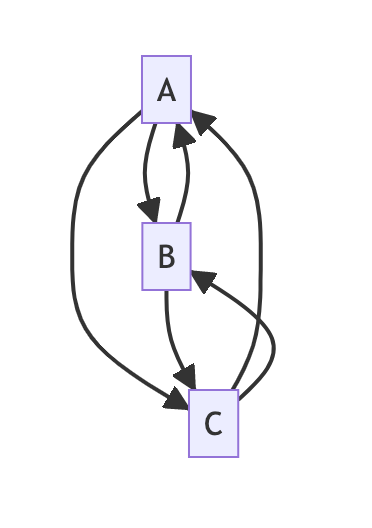
\includegraphics[width=0.3\textwidth]{images/astar.png}
\caption{Fully connected graph}
\label{fig:fully_connected_graph}
\end{figure}

The heuristic function is slightly different:

\begin{equation*}
h_i = len(s_i) - len(s_i \cap S_e)
\end{equation*}

where $s_i$ is the current subset and $S_e$ is the expected solution. It takes into account both the length of the new subset (to minimise final weight) and the number of undiscovered elements that it can contribute.

We can also immediately return a very large heuristic value such as 100 in the case of duplicating elements in the subset or in any situation where we want a certain node to be immediately skipped.

\begin{mintedbox}{python}
  class AStarSearchFullyConnectedGraph:
    def __init__(self, adjacency_list, list_values, N):
        self.adjacency_list = adjacency_list
        self.list_values = list_values
        H = {}
        for key in list_values:
            # heuristic value is length of list
            H[key] = len(list_values[key])
        self.H = H
        # holds the lists of each visited node
        self.final_list = []
        # N is the count of elements that should be in the final list
        self.N = N
        self.discovered_elements = set()

    def flatten_list(self, _list):
        return list(itertools.chain.from_iterable(_list))

    def get_neighbors(self, v):
        return self.adjacency_list[v]

    def get_number_of_elements_not_in_second_list(self, list1, list2):
        count = 0
        # flattened_list = self.flatten_list(list2)
        for i in set(list1):
            # print("i: ", i)
            if i not in list2:
                count += 1
        # if count > 1:
        #     print("count: ", count)
        return len(set(list1) - set(list2))

    # f(n) = h(n) + g(n)

    def h(self, n):
        num_new_elements = self.get_number_of_elements_not_in_second_list(self.list_values[n], self.discovered_elements)
        # if self.list_values[n] in self.final_list:
        #     return 1000
        return num_new_elements
        # return self.H[n] / (num_new_elements + 1)

    def get_node_with_least_h(self):
        min_h = float("inf")
        min_node = None
        for node in self.adjacency_list:
            if self.h(node) < min_h:
                min_h = self.h(node)
                min_node = node
        return min_node

    def get_node_with_least_h_and_not_in_final_list(self):
        min_h = float("inf")
        min_node = None
        for node in self.adjacency_list:
            if self.h(node) < min_h and node not in self.final_list:
                min_h = self.h(node)
                min_node = node
        return min_node

    # visited_node = [1, 2, 3]
    # final_list = [[4, 5], [1]]
    def are_we_done(self):
        # flattened_list = list(itertools.chain.from_iterable(self.final_list))
        for i in range(self.N):
            if i not in self.discovered_elements:
                return False
        print("We are done")
        return True

    def insert_unique_element_into_list(self, _list, element):
        if element not in _list:
            _list.append(element)
        return _list

    def a_star_algorithm(self):
        # start_node is node with lowest cost
        start_node = self.get_node_with_least_h()

        open_list = [start_node]
        closed_list = []

        g = {}

        g[start_node] = 0

        parents = {}
        parents[start_node] = start_node

        while len(open_list) > 0:
            n = None

            # find a node with the highest value of f() - evaluation function
            for v in open_list:
                if n == None or g[v] + self.h(v) > g[n] + self.h(n):
                    n = v;

            if n == None:
                print('Path does not exist!')
                return None

            print(f"Visiting node: {n}")
            self.final_list.append(self.list_values[n])
            # self.discovered_elements.union(self.list_values[n])
            # add list_values[n] to discovered_elements
            for i in self.list_values[n]:
                self.discovered_elements.add(i)
            print(len(self.discovered_elements))

            # if the current node is the stop_node
            # then we begin reconstructin the path from it to the start_node
            if self.are_we_done():
                reconst_path = []

                while parents[n] != n:
                    reconst_path.append(n)
                    n = parents[n]

                reconst_path.append(start_node)

                reconst_path.reverse()

                print(f"Number of elements in final list: {len(self.flatten_list(self.final_list))}")
                print('Path found: {}'.format(reconst_path))
                print(
                    f"My solution for N={N}: w={sum(len(_) for _ in self.final_list)} (bloat={(sum(len(_) for _ in self.final_list)-N)/N*100:.0f}%)"
                )
                return reconst_path

            # for all neighbors of the current node do
            for (m, weight) in self.get_neighbors(n):
                values = self.list_values[m]
                if m not in open_list and m not in closed_list:
                    # open_list.add(m)
                    open_list = self.insert_unique_element_into_list(open_list, m)
                    # sort open_list by self.h
                    open_list = sorted(open_list, key=self.h)
                    parents[m] = n
                    g[m] = g[n] + weight

                else:
                    if g[m] + self.h(m) > g[n] + self.h(n) + weight:
                        g[m] = g[n] + weight
                        parents[m] = n

                        # if m in closed_list:
                        #     closed_list.remove(m)
                        #     # open_list.add(m)
                        #     open_list = self.insert_unique_element_into_list(open_list, m)
                        #     open_list = sorted(open_list, key=self.h)


            open_list.remove(n)
            open_list = sorted(open_list, key=self.h)
            closed_list = self.insert_unique_element_into_list(closed_list, n)

        print('Path does not exist!')
        return None
\end{mintedbox}

\subsection{Results}

\subsection{Received Reviews}

\begin{tcolorbox}[colback=green!5!white,colframe=green!75!black,code={\singlespacing}]
  Diego Mangasco
  \tcblower
  REVIEW BY DIEGO GASCO (DIEGOMANGASCO)
SET COVERING (GREEDY):
I appreciated a lot the comparison between the professor's Naive greedy approach and your greedy approach!
The idea to implement a sort of priority function to choose the best set to add to the solution is nice (a kind of cherry picking).
I think you decided to take the set with lowest "f" because you want to keep low the total weight as you can.
What if you merge this idea with the number of new elements that the new set can bring to your solution?
You can try to find a sort of trade-off between having a new small set and having a new useful one!

SET COVERING (A* TRAVERSAL USING PRIORITY QUEUE):
In my implementation I basically used the same approach in developing my A* algorithm!
Like you, I decided to implement my heuristics as the number of undiscovered elements, and I took as cost, the length of the new set added in the solution.
I also noticed that, with cost sets as unit and not as the length of the new set, the process is much faster, but the solution that we reached is not optimal, so I decided to keep the length as cost.

The only small difference with my implementation is the use of the data structures.
To don't have to deal with list manipulation, I preferred to focused my structures in a more set-oriented way.
But never mind, these are just personal preferences!

SET COVERING (A* TRAVERSAL USING A FULLY CONNECTED GRAPH)
Unfortunately I couldn't try this implementation of A*, because I didn't understand the data structure "adjacency list" and there isn't a block that starts this piece of code like for the previous solutions
Reading your explanation about the algorithm idea, I can say that this approach can be useful with a solution space that is not huge, but can become computationally expansive with large N (due to the connections you might have to manage).
But anyway with small/medium N it can be helpful in reducing the time of the classical A*.

\end{tcolorbox}

\begin{tcolorbox}[colback=green!5!white,colframe=green!75!black,code={\singlespacing}]
  Ramin
  \tcblower
The code is written in a clear way and it's easy to understand. The code style is clear and the code is well organized in classes.
The fact that you tried to implement a sort of priority function to choose the best set to add to the solution is nice and smart.
Also you decided to implement your heuristics as the number of elements that have not been found yet, which is also a great idea.
My only question is that , what is the best way to estimate the weight, considering the new items?
\end{tcolorbox}

\begin{tcolorbox}[colback=green!5!white,colframe=green!75!black,code={\singlespacing}]
  Arman
  \tcblower
Hi Sid,

here is my review:

The algorithm you tried as an augmented greedy solution is finding good solutions for small Ns, e.g. 29 for N=20 which is close to the exact solution. (you forgot to put N=20 in the solutions as well, it's good to add it as you are using this as your baseline). The function which it uses for cost is actually a kind of heuristic used in a greedy context. It is an interesting use case. for large Ns, It does not improve the solution, although meaningfully reduces the number of visited nodes. It's a kind of behaviour we observe when using heuristics in other search algorithms as well.

for A* search, your code is pretty clean and organised  specially implementing in a class which makes it reusable. the heuristic is reasonable and simple. comparing length as cost and unit cost is useful to see the difference. My experience was that not using cost and not keeping parents did not made much difference in this specific problem and it makes code much smaller and faster.

The fact that you used the itertools methods has made your code cleaner and more elegant. It is better to implement loops, e.g. in are\_we\_done() using comprehension, using inner loops in separate line will affect the speed significantly.

Using a fully connected graph is interesting experiment, I will follow.

Bests
\end{tcolorbox}

\subsection{Given Reviews}

\subsubsection{Shayan}

Shayan's code

\begin{mintedbox}{python}
import random
import logging
logging.getLogger().setLevel(logging.INFO)

def custom_search(N, seed):
    goal = set(range(N))
    covered = set()
    solution = list()
    all_lists = problem(N, seed=42)
    random.seed(seed)
    random.shuffle(all_lists) #shuffle list to pop random
    while goal != covered: #while set of covered nums is not equal to goal
        x = all_lists.pop(0) #pick a list from all_lists
        if not set(x) < covered: #if set of picked list is not a subset of covered
            solution.append(x) #append it to the solution
            covered |= set(x) #covered gets updated and becomes a union of covered plus picked set


    logging.info(
        f"custom search solution for N={N}: w={sum(len(_) for _ in solution)} (bloat={(sum(len(_) for _ in solution)-N)/N*100:.0f}%)"
    )
logging.getLogger().setLevel(logging.DEBUG)
for N in [5, 10, 20, 100, 500, 1000]:
    custom_search(N, 99)
\end{mintedbox}

Hi Shayan,

I had a look at your code and had a few thoughts:

1. You seem to be using a completely random approach to solving the problem, making a random, uninformed choice at each iteration of the loop. When running the algorithm with different random seeds, a different bloat factor and $w$ are produced. The gist is that picking subsets randomly neither guarantees a heuristically optimal solution nor is the runtime optimised.

2. One suggestion to make informed decisions when choosing subsets is to sort the list by undiscovered elements / length of the list / other factors that affect the efficiency of the solution. This would still be a greedy, heuristically approximate solution that could improve both performance and runtime. Furthermore, you could consider traversing the list through more powerful search algorithms such as Djikstra or A-Star.

2. (Miscellaneous) While the results are in the notebook, perhaps you can add them to the markdown file to compare it with other algorithms in the future.

Thank you! If there are any other details I can add, please do let me know.

\subsubsection{Arman}

Arman's code

\begin{mintedbox}{python}
    import enum
    from itertools import count
    import logging
    import random
    from gx_utils import *
    from heapq import heappush
    from typing import Callable
    import statistics
    # import queues

    logging.basicConfig(format="%(message)s", level=logging.INFO)

    N = 1000
    NUMBERS = {x for x in range(N)}


    def problem(N, seed=None):
        random.seed(seed)
        return [
            list(set(random.randint(0, N - 1) for n in range(random.randint(N // 5, N // 2))))
            for n in range(random.randint(N, N * 5))
        ]

    class State:
        def __init__(self, list_numbers:set):
            self.lists_ = list_numbers.copy()
        def add(self,item):
            self.lists_.add(item)
            return self
        def __hash__(self):
            #return hash(bytes(self.lists_))
            return hash(str(self.lists_))
        def __eq__(self, other):
            #return bytes(self.lists_) == bytes(other.lists_)
            return str(self.lists_) == str(other.lists_)
        def __lt__(self, other):
            #return bytes(self.lists_) < bytes(other.lists_)
            return str(self.lists_) < str(other.lists_)
        def __str__(self):
            return str(self.lists_)
        def __repr__(self):
            return repr(self.lists_)
        def copy_data(self):
            return self.lists_.copy()
        def get_weight(self,ref_lists):
            return len([x for n in self.lists_ for x in ref_lists[n]])
        def get_items(self,ref_lists):
            return set([x for n in self.lists_ for x in ref_lists[n]])


    def goal_test(current_state:State,ref_lists):
        """get all the members of the lists in the current_state and check if it covers N"""

        current_numbers = {x for n in current_state.lists_ for x in ref_lists[n]}
        return current_numbers == NUMBERS

    def valid_actions(current_state:State,ref_lists):
        """returns set of indexes not currently added to this state"""
        return {indx for indx,_ in enumerate(ref_lists) if indx not in current_state.lists_}

    def result(current_state,action):
        next_state=State(current_state.copy_data()).add(action)
        return next_state

    def search(initial_state:State, ref_lists,priority_function:Callable):
        frontier = PriorityQueue()
        state = initial_state
        state_count = 0
        while state is not None and not goal_test(state,ref_lists):
            for a in valid_actions(state,ref_lists):
                new_state = result(state,a)
                if new_state not in frontier:
                    frontier.push(new_state,p=priority_function(new_state))
                elif new_state in frontier:
                    pass
            if frontier:
                state = frontier.pop()
                state_count+=1
            else:
                state = None

        logging.info(f"Found a solution with cost: {state.get_weight(ref_lists)} and {state_count} number of visited states, last state: {state}")

    def heuristic(state:State,ref_lists,N):
        remained = NUMBERS - state.get_items(ref_lists)
        return len(remained) + random.randint(0,len(remained)//2)


    if __name__ == "__main__":
        ref_lists = problem(N,seed=42)
        #print(ref_lists)
        initial_state = State(set())

        # #Breath_first
        # search(initial_state, ref_lists,priority_function=lambda state: state.get_weight(ref_lists))

        # #Depth_first
        # search(initial_state, ref_lists,priority_function=lambda state: -state.get_weight(ref_lists))

        # #Heuristic
        search(initial_state, ref_lists,priority_function=lambda state: heuristic(state,ref_lists, N))
\end{mintedbox}

Hi Arman,

Here are my observations with regard to your solution for Lab 1:

1. The priority queue is a suitable choice to store and select subsets in each iteration of your loop. All 4 traversal algorithms are compared by editing the priority function, and similar to mine, A-star performed best.

2. Your heuristic function is particularly interesting because it combines the "potential new elements" with a random number.

\begin{mintedbox}{python}
def heuristic(state:State,ref_lists,N):
    remained = NUMBERS - state.get_items(ref_lists)
    return len(remained) + random.randint(0,len(remained)//2)
\end{mintedbox}

There also wasn't an explanation in the Readme, so I'm very curious as to the reason behind this heuristic. I ran your code with and without this random component and found that using it improves performance for larger values of N such as $N=100$ or $N=500$, but not so for smaller values like $N=20$. If you could add an explanation to your Readme about the heuristic, I would be very interested to read it.

3. Your algorithm does not hit a bottleneck for values of $N>50$, in which case most people's code "exploded". Therefore, any solution, though not necessarily optimal, is reached.

4. One suggestion I have is to experiment with other heuristic functions, such as those that consider both the number of attainable new elements and the length of the incoming subset.
%!TEX ROOT = main.tex

\section{Lab 2}

\subsection{Solution}

In this lab, we will take a GA approach to solving the set-covering problem. As a background, let's assume we have 500 potential lists that should form a complete subset.

The final product should be a list of 0s and 1s that indicate which lists should be included in the final set. We use a genetic approach to obtain this list via:

\begin{enumerate}
  \item Mutation: randomly change a 0 to a 1 or vice versa
  \item Crossover: randomly select a point in the list and swap the values after that point
\end{enumerate}

\subsubsection{Representing the problem}
We will represent the problem as a list of 0s and 1s. The length of the list will be the number of lists we have. The 0s and 1s will indicate whether or not the list should be included in the final set.

The objective of the algorithm is to find an optimal (or at least as optimal as possible) set of 0s and 1s that will cover all the elements in the list.

\subsubsection{Assessing Fitness}

Based on knowledge obtained in previous labs, the heuristic function evolved and these were the factors I considered:

\begin{enumerate}
  \item Potential duplicates
  \item Undiscovered elements
  \item Length of subset
\end{enumerate}

The following equations were formulated for fitness assessment:

\begin{equation}
  len(distinct\_elements)
\end{equation}

\begin{equation}
  len(distinct\_elements) / (num\_duplicates + 1)
\end{equation}

\begin{equation}
  len(distinct\_elements) / (num\_duplicates + 1) - num\_undiscovered\_elements
\end{equation}

\begin{equation}
  len(distinct\_elements) / (num\_undiscovered\_elements + 1)
\end{equation}

After multiple trials, the best fitness function is the simplest, which is simply the number of distinct elements.

\subsection{Results}

The following are the results of the algorithm after 1000 generations (only the best results are reported):

\begin{table}
  \centering
  \begin{tabular}{|c|c|}
    \hline
    N & W \\
    \hline
    5 & . \\
    10 & 10 \\
    20 & 24 \\
    50 & 100 \\
    100 & 197 \\
    500 & 1639 \\
    1000 & 3624 \\
    \hline
  \end{tabular}
  \caption{Results of the algorithm}

\end{table}

With larger values of $N$, a smaller population and offspring size is sufficient. Early stopping is used to detect the plateau, so the algorithm doesn't run endlessly. However, the minima is often reached in less than 100 generations.

\subsubsection{The Case of Mutations}

\paragraph{Plateau Detection and Dynamic Change of Mutation Rate}

Based on the rate of change of the fitness, the mutation rate (number of elements in genome to mutate) is adjusted.

\begin{mintedbox}{python}
def choose_mutation_rate(fitness_log):
  # choose mutation rate based on change in fitness_log
  if len(fitness_log) == 0:
      return 0.2
  if len(fitness_log) < 3:
      considered_elements = len(fitness_log)
  else:
      considered_elements = 3
  growth_rate = np.mean(np.diff(fitness_log[-considered_elements:]))
  if growth_rate <= 0:
      return 0.4
  elif growth_rate < 0.5:
      return 0.3
  elif growth_rate < 1:
      return 0.01
  else:
      return 0.1

def plateau_detection(num_generations, fitness_log):
  '''
  Checks if the fitness has plateaued for the last num_generations.
  '''
  # this function is not used
  return all(fitness_log[-num_generations] == fitness_log[-i] for i in range(1, num_generations))
\end{mintedbox}

\subsection{Mutation Functions}

\subsubsection{Flip Mutation}

\begin{mintedbox}{python}
  def flip_mutation(genome, mutate_only_one_element=False):
    '''
    Flips random bit(s) in the genome.
    Parameters:
    mutate_only_one_element: If True, only one bit is flipped.
    '''
    modified_genome = genome.copy()
    if mutate_only_one_element:
        # flip a random bit
        index = random.randint(0, len(modified_genome) - 1)
        modified_genome[index] = 1 - modified_genome[index]
    else:
        # flip a random number of bits
        num_to_flip = choose_mutation_rate(fitness_log) * len(modified_genome)
        to_flip = random.sample(range(len(modified_genome)), int(num_to_flip))
        # to_flip = random.sample(range(len(modified_genome)), random.randint(0, len(modified_genome)))
        modified_genome = [1 - modified_genome[i] if i in to_flip else modified_genome[i] for i in range(len(modified_genome))]

    # mutate only if it brings some benefit to the weight
    # if calculate_weight(modified_genome) < calculate_weight(genome):
    #     return modified_genome

    return return_best_genome(modified_genome, genome)
\end{mintedbox}

\subsubsection{Scramble Mutation}

\begin{mintedbox}{python}
def scramble_mutation(genome):
  '''
  Randomly scrambles the genome.
  '''
  # select start and end indices to scramble
  modified_genome = genome.copy()
  start = random.randint(0, len(modified_genome) - 1)
  end = random.randint(start, len(modified_genome) - 1)
  # scramble the elements
  modified_genome[start:end] = random.sample(modified_genome[start:end], len(modified_genome[start:end]))
  return return_best_genome(modified_genome, genome)
\end{mintedbox}

\subsubsection{Swap Mutation}

\begin{mintedbox}{python}
def swap_mutation(genome):
  '''
  Randomly swaps two elements in the genome.
  '''
  modified_genome = genome.copy()
  index1 = random.randint(0, len(modified_genome) - 1)
  index2 = random.randint(0, len(modified_genome) - 1)
  modified_genome[index1], modified_genome[index2] = modified_genome[index2], modified_genome[index1]
  return return_best_genome(modified_genome, genome)
\end{mintedbox}

\subsubsection{Inversion Mutation}

\begin{mintedbox}{python}
def inversion_mutation(genome):
  '''
  Randomly inverts the genome.
  '''
  modified_genome = genome.copy()
  # select start and end indices to invert
  start = random.randint(0, len(modified_genome) - 1)
  end = random.randint(start, len(modified_genome) - 1)
  # invert the elements
  modified_genome = modified_genome[:start] + modified_genome[start:end][::-1] + modified_genome[end:]
  return return_best_genome(modified_genome, genome)
\end{mintedbox}

\subsection{Full Code}

\begin{mintedbox}{python}
import numpy as np
import itertools

def calculate_fitness(genome):
    '''
    Calculates the fitness of the given genome.
    The fitness is the number of unique elements
    The weight is the total number of elements in the genome
    '''
    # fitness is number of distinct elements in genome
    all_elements = []
    distinct_elements = set()
    weight = 0
    for subset, gene in zip(prob, genome):
        # if the particular element should be taken
        if gene == 1:
            distinct_elements.update(subset)
            weight += len(subset)
            all_elements += subset
    num_duplicates = len(all_elements) - len(set(all_elements))
    num_undiscovered_elements = len(set(range(N)) - distinct_elements)
    # print(set(range(N)) - distinct_elements)
    # print("num_undiscovered_elements", num_undiscovered_elements)
    # return num_undiscovered_elements, -weight
    # return len(distinct_elements), -weight
    # return num_undiscovered_elements / (len(distinct_elements) + 1), -weight
    return len(distinct_elements) / (num_undiscovered_elements + 1), -weight
    # other potential fitness functions:
    # return len(distinct_elements) / (num_duplicates + 1)
    # return len(distinct_elements) / (num_duplicates + 1) - num_undiscovered_elements, -weight
    # return len(distinct_elements) / (num_undiscovered_elements + 1), -weight

def generate_element():
    '''
    Randomly generates offspring made up of 0s and 1s.
    1 means the element is taken, 0 means it is not.
    '''
    genome = [random.randint(0, 1) for _ in range(N)]
    fitness = calculate_fitness(genome)
    # genome = np.random.choice([True, False], size=PROBLEM_SIZE)
    return Individual(genome, fitness)

initial_population = [generate_element() for _ in range(POPULATION_SIZE)]

len(initial_population)

fitness_log = []

def calculate_weight(genome):
    '''
    Weight Function
    Weight is the sum of the lengths of the subsets that are taken
    '''
    # select the subsets from prob based on the best individual
    final = [prob[i] for i, gene in enumerate(genome) if gene == 1]
    weight = len(list(itertools.chain.from_iterable(final)))
    return weight

def choose_mutation_rate(fitness_log):
    # choose mutation rate based on change in fitness_log
    if len(fitness_log) == 0:
        return 0.2
    if len(fitness_log) < 3:
        considered_elements = len(fitness_log)
    else:
        considered_elements = 3
    growth_rate = np.mean(np.diff(fitness_log[-considered_elements:]))
    if growth_rate <= 0:
        return 0.4
    elif growth_rate < 0.5:
        return 0.3
    elif growth_rate < 1:
        return 0.01
    else:
        return 0.1

def plateau_detection(num_generations, fitness_log):
    '''
    Checks if the fitness has plateaued for the last num_generations.
    '''
    if len(fitness_log) < num_generations:
        return False
    return all(fitness_log[-num_generations] == fitness_log[-i] for i in range(1, num_generations))

def flip_mutation(genome, mutate_only_one_element=False):
    '''
    Flips random bit(s) in the genome.
    Parameters:
    mutate_only_one_element: If True, only one bit is flipped.
    '''
    modified_genome = genome.copy()
    if mutate_only_one_element:
        # flip a random bit
        index = random.randint(0, len(modified_genome) - 1)
        modified_genome[index] = 1 - modified_genome[index]
    else:
        # flip a random number of bits
        num_to_flip = choose_mutation_rate(fitness_log) * len(modified_genome)
        to_flip = random.sample(range(len(modified_genome)), int(num_to_flip))
        # to_flip = random.sample(range(len(modified_genome)), random.randint(0, len(modified_genome)))
        modified_genome = [1 - modified_genome[i] if i in to_flip else modified_genome[i] for i in range(len(modified_genome))]

    return modified_genome
    # mutate only if it brings some benefit to the weight
    # if calculate_weight(modified_genome) < calculate_weight(genome):
    #     return modified_genome


def return_best_genome(genome1, genome2):
    return genome1
    # if calculate_fitness(genome1) > calculate_fitness(genome2):
    #     return genome1
    # else:
    #     return genome2

def mutation(genome):
    '''
    Runs a randomly chosen mutation on the genome. Mutations are:
    1. Bit Flip Mutation
    2. Scramble Mutation
    3. Swap Mutation
    4. Inversion Mutation
    Refer to README for more details.
    '''
    # check type of genome (debugging)
    # if type(genome) == tuple:
    #     print("genome is tuple")
    #     print(genome)

    possible_mutations = [flip_mutation, scramble_mutation, swap_mutation, inversion_mutation]
    chosen_mutation = random.choice(possible_mutations)
    return chosen_mutation(genome)

    # if random.random() < 0.1:
    #     for _ in range(num_elements_to_mutate):
    #         index = random.randint(0, len(genome) - 1)
    #         genome[index] = 1 - genome[index]
    # mutate a random number of elements
    # to_flip = random.randint(0, len(genome))
    # # flip the bits
    # return [1 - genome[i] if i < to_flip else genome[i] for i in range(len(genome))]

def scramble_mutation(genome):
    '''
    Randomly scrambles the genome.
    '''
    # select start and end indices to scramble
    modified_genome = genome.copy()
    start = random.randint(0, len(modified_genome) - 1)
    end = random.randint(start, len(modified_genome) - 1)
    # scramble the elements
    modified_genome[start:end] = random.sample(modified_genome[start:end], len(modified_genome[start:end]))
    return return_best_genome(modified_genome, genome)

def swap_mutation(genome):
    '''
    Randomly swaps two elements in the genome.
    '''
    modified_genome = genome.copy()
    index1 = random.randint(0, len(modified_genome) - 1)
    index2 = random.randint(0, len(modified_genome) - 1)
    modified_genome[index1], modified_genome[index2] = modified_genome[index2], modified_genome[index1]
    return return_best_genome(modified_genome, genome)

def inversion_mutation(genome):
    '''
    Randomly inverts the genome.
    '''
    modified_genome = genome.copy()
    # select start and end indices to invert
    start = random.randint(0, len(modified_genome) - 1)
    end = random.randint(start, len(modified_genome) - 1)
    # invert the elements
    modified_genome = modified_genome[:start] + modified_genome[start:end][::-1] + modified_genome[end:]
    return return_best_genome(modified_genome, genome)

def crossover(genome1, genome2):
    '''
    Crossover the two genomes by randomly selecting a point
    '''
    # crossover at a random point
    crossover_point = random.randint(0, len(genome1))
    modified_genome = genome1[:crossover_point] + genome2[crossover_point:]
    return modified_genome

def roulette_wheel_selection(population):
    '''
    Selects an individual from the population based on the fitness.
    '''
    # calculate the total fitness of the population
    total_fitness = sum([individual.fitness[0] for individual in population])
    # select a random number between 0 and the total fitness
    random_number = random.uniform(0, total_fitness)
    # select the individual based on the random number
    current_fitness = 0
    for individual in population:
        current_fitness += individual.fitness[0]
        if current_fitness > random_number:
            return individual

def stochastic_universal_sampling(population):
    '''
    Select using Stochastic Universal Sampling.
    '''
    point_1 = random.uniform(0, 1)
    point_2 = point_1 + 1
    # In Progress

def rank_selection(population):
    '''
    Select using Rank Selection. Read more here:
    https://www.tutorialspoint.com/genetic_algorithms/genetic_algorithms_parent_selection.htm
    '''
    # sort the population based on the fitness
    population.sort(key=lambda x: x.fitness[0], reverse=True)
    # calculate the total rank
    total_rank = sum([i for i in range(len(population))])
    # select a random number between 0 and the total rank
    random_number = random.uniform(0, total_rank)
    # select the individual based on the random number
    current_rank = 0
    for i, individual in enumerate(population):
        current_rank += i
        if current_rank > random_number:
            return individual


def tournament(population, selection_method='tournament'):
    '''
    Selects the best individual from a random sample of the population.
    '''
    if selection_method == 'roulette':
        participant = roulette_wheel_selection(population)
        participant = Individual(participant.genome, participant.fitness)
    elif selection_method == 'rank':
        participant = rank_selection(population)
        participant = Individual(participant.genome, participant.fitness)
    else:
        participant = max(random.sample(population, k=2), key=lambda x: x.fitness)
        participant = Individual(participant.genome, participant.fitness)
    return participant

def generate(population, generation):
    '''
    Create offspring from the population using either:
    1. Cross Over + Mutation
    2. Mutation
    '''
    # can either cross over between two parents or mutate a single parent
    if random.random() < 0.2:
        parent = tournament(population)
        # if random.random() <= 0.3:
        #     genome = mutation(parent.genome)
        genome = mutation(parent.genome)
        child = Individual(parent, calculate_fitness(parent))
    else:
        # crossover
        parent1 = tournament(population)
        parent2 = tournament(population)
        genome = crossover(parent1.genome, parent2.genome)
        # if random.random() <= 0.3:
        #     genome = mutation(genome)
        genome = mutation(genome)
        child = Individual(genome, calculate_fitness(genome))

    fitness_log.append((generation + 1, child.fitness[0]))

    return child

    best = max(initial_population, key=lambda x: x.fitness)

    best_individual = max(initial_population, key=lambda x: x.fitness)
    for i in range(NUM_GENERATIONS):
        # create offspring
        offspring = [generate(initial_population, i) for i in range(OFFSPRING_SIZE)]
        # calculate fitness
        # offspring = [Individual(child.genome, calculate_fitness(child.genome)) for child in offspring]

        initial_population = initial_population + offspring
        initial_population = sorted(initial_population, key=lambda x: x.fitness, reverse=True)[:POPULATION_SIZE]

        fittest_offspring = max(initial_population, key=lambda x: x.fitness)

        if fittest_offspring.fitness > best_individual.fitness:
            best_individual = fittest_offspring

    # get the best individual
    print(calculate_weight(best_individual.genome))
\end{mintedbox}

\subsection{Received Reviews}

\begin{tcolorbox}[colback=green!5!white,colframe=green!75!black,code={\singlespacing}]
    s295103
    \tcblower
    Your commitment to this lab can be seen from all the approaches you implemented and tested.
    My only issue is with the plateau detection function that is bound to always return False in that implementation.
    Also a suggestion: try to enforce the constraint that all individuals' genome must be a solution with full set cover; in this way you'll vastly reduce the search space.
\end{tcolorbox}

  \begin{tcolorbox}[colback=green!5!white,colframe=green!75!black,code={\singlespacing}]
    s295103
    \tcblower

  Design considerations
  - Overall good solution, nice work trying multiple parent selection functions, different fitness functions, and using multiple mutation functions

  Implementation considerations
  - After calling the problem() function it is necessary to reset the seed to a random value using `random.seed()` otherways all runs will always use 42 as seed value, so they won't be truly random

  \begin{mintedbox}{python}
    def flip_mutation(genome, mutate_only_one_element=False): is never called with mutate_only_one_element=True
    genome = mutation(parent.genome)
    child = Individual(parent, calculate_fitness(parent))
  \end{mintedbox}

  should substituted by

  \begin{mintedbox}{python}
    genome = mutation(parent.genome)
    child = Individual(genome, calculate_fitness(genome))
    \end{mintedbox}

    for the mutation to have effect, since in every mutation you do

    \begin{mintedbox}{python}

    def *_mutation(genome):
	modified_genome = genome.copy()
	...
	return modified_genome
\end{mintedbox}

\begin{mintedbox}{python}
    initial_population = sorted(initial_population, key=lambda x: x.fitness, reverse=True)[:POPULATION_SIZE]
fittest_offspring = max(initial_population, key=lambda x: x.fitness)
\end{mintedbox}

can become

\begin{mintedbox}{python}
initial_population = sorted(initial_population, key=lambda x: x.fitness, reverse=True)[:POPULATION_SIZE]
fittest_offspring = initial_population[0]
\end{mintedbox}

  so that you don't need to search for the max in the list you just sorted
  - The README and the important parts of the code are very clean and structured, but there are some comments, unused functions, an unfinished function, and other parts of the file that can be cleaned up a little
\end{tcolorbox}

\begin{tcolorbox}[colback=green!5!white,colframe=green!75!black,code={\singlespacing}]
   Ricardo Nicida Kazama
\tcblower
In the README, I was wondering if the function $return\_best\_genome$($modified\_genome$, genome) might disturb the exploration of your algorithm since a worse solution that could go towards the global optimum might be chosen instead of the current better solution that is going to a local optimum. Analyzing your code, I notice that the part where you would compare the genomes to pick the best is commented. Therefore, maybe you experienced what I previously mentioned.
In the following part of the code, the use of the iterator "i" is a bit confusing since the one being taken into account for the function generate($initial\_population$, i) is the one in range($OFFSPRING\_SIZE$). However, from what I understood, the second input should be the generation number.

\begin{mintedbox}{python}

for i in range(NUM_GENERATIONS):
    # create offspring
    offspring = [generate(initial_population, i) for i in range(OFFSPRING_SIZE)]
\end{mintedbox}

Highlights/overall:
The solution includes many different mutations which show an extra effort to improve the results with a broad approach.
The change in the mutation rate based on the $fitness\_log$ is an interesting idea and seems to be effective.
The code and results are very good!
\end{tcolorbox}

\subsection{Given Reviews}

\subsubsection{Erik}

Erik's code

\begin{mintedbox}{python}
# Should be used to init solution space, return a list of list
def select_rand_solution(full_input):
    population = []
    random.seed(None)
    for i in range(POPULATION_SIZE):
        population.append(random.sample(full_input, random.randint(1, len(full_input))))
    return population


# check if one solution is valid
def goal_check(curr):
    curr = [item for sublist in curr for item in sublist]
    return set(curr) == set(range(N))


def fitness_function(entry, goal_set):
    duplicates = len(entry) - len(set(tuple(entry)))
    miss = len(goal_set.difference(set(entry)))
    return (-1000 * miss) - duplicates


def calculate_fitness(individual):
    flat_individual = [item for sublist in individual for item in sublist]
    fitness_val = fitness_function(flat_individual, set(range(N)))
    return fitness_val


def select_parents(population):
    nr_of_boxes = int(POPULATION_SIZE * (POPULATION_SIZE + 1) / 2)
    random.seed(None)
    random_wheel_nr = random.randint(1, nr_of_boxes)
    parent_number = POPULATION_SIZE
    increment = POPULATION_SIZE - 1
    curr_parent = 0
    while random_wheel_nr > parent_number:
        curr_parent += 1
        parent_number += increment
        increment -= 1
    return population[curr_parent]


# randomize an index and merge 0-index from parent 1 and index-len of parent two, mutate with 5% chance
def crossover(first_parent, second_parent):
    slice_index_one = random.randint(0, min(len(first_parent[0]) - 1, len(second_parent[0]) - 1))
    child = first_parent[0][:slice_index_one] + second_parent[0][slice_index_one:]
    return child


# mutate child and return
def mutate_child(individual, problem_space):
    index = random.randint(0, len(individual) - 1)
    random_list = problem_space[random.randint(0, len(problem_space) - 1)]
    random_gene = random_list[random.randint(0, len(random_list) - 1)]
    individual = individual[:index] + individual[index+1:] + [random_gene]
    return individual


def update_population(population, new_children):
    new_population = population + new_children
    sorted_population = sorted(new_population, key=lambda i: i[1], reverse=True)
    return sorted_population[:POPULATION_SIZE]


def main():
    logging.basicConfig(level=logging.DEBUG)
    problem_space = problem(N, seed=42)
    population = select_rand_solution(problem_space)

    # should hold current population with the calculated fitness
    current_individuals = []

    # setup data structure, list of tuples containing ([entries], fitness) and sort
    for individual in population:
        current_individuals.append((individual, calculate_fitness(individual)))

    current_individuals = sorted(current_individuals, key=lambda l: l[1], reverse=True)

    counter = 0
    while counter < NR_OF_GENERATIONS:
        # a) Select individuals with a good fitness score for reproduction.
        cross_over_list = []
        for i in range(OFFSPRING_SIZE):
            parent_one = select_parents(current_individuals)
            parent_two = select_parents(current_individuals)

            # b) Let them produce offspring. Mutate with 5% chance
            tmp_child = crossover(parent_one, parent_two)
            if random.random() > 0.95:
                tmp_child = mutate_child(tmp_child, population)

            cross_over_list.append((tmp_child, calculate_fitness(tmp_child)))

        current_individuals = update_population(current_individuals, cross_over_list)
        counter += 1

    for solution in current_individuals:
        if goal_check(solution[0]):
            logging.info(f'Best solution for N={N} was {current_individuals[0][0]} \nWith a weight of {sum(len(_) for _ in current_individuals[0][0])}')
            break
\end{mintedbox}

Hi Eric,

Here's my review concerning your approach to lab 2.

There are a few high-level, cosmetic attributes you did well:
1. Each function is well-documented and well-labelled, so I could easily understand the purpose of each one. One way to improve could be to leverage Python docstrings, where you can also explain input parameters and output values. To do this, add:

\begin{mintedbox}{python}
def mutation(genome):
  '''
  Function mutates genome using .... strategy, etc.
  args:
  genome: str - Input genome
  '''
\end{mintedbox}

3. Using a Python script made it easy for me to run code iteratively for many different values of N/Offspring sizes/etc. without having to run all the cells. I was able to reproduce your best results after a few tries.

Let's break down the solution itself:

1. I noticed that you leveraged a completely random roulette-wheel-based selection, which leverages completely on random chance, compared to a fitness-based tournament selection which performed better (at least from my experience with this lab). Perhaps, you could try experimenting with different parent selection methods instead of just one. \\

2. Your fitness function is particularly interesting, standing out from most others I've seen. It takes into account duplicates in the subset:

\begin{mintedbox}{python}
  def fitness_function(entry, goal_set):
    duplicates = len(entry) - len(set(tuple(entry)))
    miss = len(goal_set.difference(set(entry)))
    return (-1000 * miss) - duplicates
\end{mintedbox}

I understand that the infinitesimal blowup by $*1000$ may theoretically help punish the algorithm if it is far from the goal. I modified your code with 2 different fitness functions:

\begin{mintedbox}{python}
  return miss-duplicates
\end{mintedbox}

\begin{mintedbox}{python}
  return (-1000 * miss)-duplicates
\end{mintedbox}

and the results were the same, so I look forward to reading about your motivation for this in the README.

Since you're only subtracting the two values (one is much larger than the other), you can do 1 of 2 things to improve convergence: divide the values, or return them as a tuple (like we did for the first lab).
You could also try different mathematical equations for the fitness function, that takes into account duplicates, undiscovered elements, length, etc., kind of like the heuristic functions we used early for graph algorithms.

3. Only one type of mutation is used (randomly flipping a bit). You could try other mutation methods and randomly choose between them to increase exploration power.

4. The probability to decide whether to mutate is quite high. In the Telegram chat, most people reported that mutations were detrimental to reaching minima, so I understand why you might have limited your mutations, but perhaps you could vary this number based on the changing fitness. Perhaps, mutate more often/more extensively to explore and reduce the vigour to exploit. You can also experiment with permutations of evolution like recombination + mutation, recombination only, mutation only, etc. All these contribute to the exploration power of your approach.

5. There is definitely a scaling problem for large values of N, such as $N=1000$. One thing to note is that minima is often reached within a fraction of 1000 generations (I logged your generational results out).

5. Representing the problem space as 0s and 1s could result in cleaner code and faster computation, but this is more of a personal preference and does not really affect the solution.

All in all, good job! I just want to read more about your exciting fitness function. Let's discuss below!

\subsubsection{Karl}

Karl's code

\begin{mintedbox}{python}
  # helping functions

def lists_to_set(genome):
    """
    convert genome to set
    :param genome: the sub-lists with random integers between 0 and N-1
    :return: set of contained elements in the genome
    """
    list_elems = [single_elem for l in genome for single_elem in l]
    s = set(list_elems)
    return s

# find out how many duplicates there are in the population
def count_duplicates(genome):
    """
    Count how many duplicates there are in the genome
    :param genome: the sub-lists with random integers between 0 and N-1
    :return: the count
    """
    list_elems = [single_elem for l in genome for single_elem in l]
    duplicates = sum([len(list(group))-1 for key, group in groupby(sorted(list_elems))])
    return duplicates
# to initialize the population
def create_population(STATE_SPACE, GOAL):
    """
    Initialize the population.
    :param STATE_SPACE: List of lists generated from problem-function
    :param GOAL: set of integers from 0 to N-1
    :return: a list of tuples: (genome,fitness), for each individual in the population.
    """
    population = []
    for _ in range(POPULATION_SIZE):
        individual = []
        for _ in range(random.randint(1,len(STATE_SPACE))):
            l = random.choice(STATE_SPACE)
            if l not in individual: #check duplicates here
                individual.append(l)
        #individual = random.choices(STATE_SPACE,k=random.randint(1,len(STATE_SPACE)))
        fitness = compute_fitness(individual, GOAL)
        population.append((individual,fitness))
    return population

def compute_fitness(genome, GOAL):
    """
    fitness is a tuple of (-#of_elems_missing,-#duplicates) which should be maximized
    :param genome: the sub-lists with random integers between 0 and N-1
    :param GOAL: set of integers from 0 to N-1
    :return: the fitness
    """
    # violated constraints, i.e. how many elements are missing
    vc = GOAL.difference(lists_to_set(genome))
    duplicates = count_duplicates(genome)
    # it is worse to lack elements than having duplicates
    fitness = (-len(vc), -duplicates)
    return fitness

def goal_check(genome, GOAL):
    """
    Check if all required elements are in the genome
    :param genome: the sub-lists with random integers between 0 and N-1
    :param GOAL: set of integers from 0 to N-1
    :return: boolean value if goal reached or not
    """
    return GOAL==lists_to_set(genome)

def parent_selection(population):
    """
    parent selection using ranking system
    P(choose fittest parent) = POPULATION_SIZE/n_slots
    P(choose second fittest parent) = (POPULATION_SIZE-1)/n_slots
    ...
    P(choose least fit parent) = 1/n_slots
    :param population: list of individuals
    :return: parent to generate offspring
    """
    ranked_population = sorted(population, key=lambda t : t[1], reverse=True)
    # number of slots in spinning wheel = POPULATION_SIZE(POPULATION_SIZE+1)/2 (arithmetic sum)
    n_slots = POPULATION_SIZE*(POPULATION_SIZE+1)/2
    wheel_number = random.randint(1,n_slots)
    curr_parent = 0
    parent_number = POPULATION_SIZE
    increment = POPULATION_SIZE-1
    while wheel_number > parent_number:
        curr_parent +=1
        parent_number +=increment
        increment -= 1
    return ranked_population[curr_parent]

# make one child from each cross-over, and mutate with low prob
def cross_over(parent1, parent2, STATE_SPACE, mutation_prob = 0.1):
    """
    Compute cross-over between two selected parents. Mutate child with mutation_prob.
    :param parent1: individual
    :param parent2: individual
    :param STATE_SPACE: List of lists generated from problem-function
    :param mutation_prob: the probability to perform mutation
    :return: the child created
    """
    cut1 = random.randint(0,len(parent1[0]))
    cut2 = random.randint(0,len(parent2[0]))
    child = parent1[0][:cut1]+parent2[0][cut2:]
    if random.random() < mutation_prob:
        mutate(child, STATE_SPACE)
    return child


def mutate(child, STATE_SPACE):
    """
    Replace one list in the child with a random one from the state space.
    :param child:
    :param STATE_SPACE:
    :return: the mutated child
    """
    idx = random.randint(0,len(child))
    #child = child[:idx] + child[idx+1:] + STATE_SPACE[random.randint(0,len(STATE_SPACE)-1)]
    i = 0
    while i<10:
        i+=1
        if STATE_SPACE[random.randint(0,len(STATE_SPACE)-1)] not in child:
             child = child[:idx] + child[idx+1:] + STATE_SPACE[random.randint(0,len(STATE_SPACE)-1)]
             break
    return child

def update_population_plus(population, offspring):
    """
    Using the plus strategy to update population to next generation.
    :param population:
    :param offspring:
    :return: the best individuals in union(population, offspring)
    """
    tot = population + offspring
    ranked_population = sorted(tot, key=lambda t : t[1], reverse=True)
    return ranked_population[:POPULATION_SIZE]

def update_population_comma(offspring):
    """
    Using the plus strategy to update population to next generation.
    :param offspring:
    :return: the best individuals in from offspring
    """
    ranked_pop = sorted(offspring, key=lambda t : t[1], reverse=True)
    return ranked_pop[:POPULATION_SIZE]

def update_mutation_prob(best_solution, best_this_iter, mutation_param, it):
    """
    Update the mutation probability according to how the performance evolves. If no improvement, mutation probability increases (favour exploration). If improvement, mutation probability decreases (favour exploitation).
    :param best_solution: The best solution so far
    :param best_this_iter: The best solution of this generation
    :param mutation_param:
    :param it: iteration number
    :return: the new mutation probability
    """
    if best_solution[1] >= best_this_iter[1]:
        mutation_param +=1
    elif best_solution[1] >= best_this_iter[1] and mutation_param>0:
        mutation_param -= 1
    return mutation_param/(1+it), mutation_param
def solve_problem(N):
    STATE_SPACE = problem(N,seed=42)
    GOAL = set(range(N))
    population = create_population(STATE_SPACE, GOAL)
    best_sol = population[0] #to be updated after each iter
    found_in_iter = 0 #to be updated
    mutation_param = 1 #increase if solution doesn't improve
    mutation_prob = 0.1 #init value
    for i in range(ITERS):
        offspring = []
        for __ in range(OFFSPRING_SIZE):
            parent1, parent2 = parent_selection(population), parent_selection(population)
            child = cross_over(parent1,parent2, STATE_SPACE, mutation_prob)
            child_fitness = compute_fitness(child, GOAL)
            offspring.append((child,child_fitness))
        population = update_population_plus(population, offspring)
        #population = update_population_comma(offspring)
        best_curr = sorted(population, key=lambda l:l[1], reverse=True)[0]
        mutation_prob, mutation_param = update_mutation_prob(best_sol, best_curr, mutation_param, i)
        if goal_check(best_curr[0],GOAL) and best_curr[1] > best_sol[1]:
            best_sol = best_curr
            found_in_iter = i
    logging.info(f'Best solution found in {found_in_iter} iters and has weight {-best_sol[1][1]}')
    return best_sol
# main

# settings
POPULATION_SIZE = 50
OFFSPRING_SIZE = 30
ITERS = 100

for N in [5,10,20,50,100,1000,2000]:
    best_sol = solve_problem(N)
    print(f'N = {N}')
    logging.info(f'The best weight for N = {N}: {-best_sol[1][1]+N}')
\end{mintedbox}

Hi Karl,

Here's my review about your approach to lab 2.
The key positives (cosmetic and logical):

1. The notebook is well-documented and cells are used appropriately. I also like that you described the steps of the algorithm before implementing it.

2. You were the only other person who compared both the (parent, offspring) and (parent + offspring) method for the algorithm. As evident in the results, parent + offspring produced more optimal weights for smaller values of $N$.

3. Parent selection also accounts for the second and third-best genomes, which could add more diversity to the selection algorithm. I don't fully understand how your wheel selection works and would love to read more about this either through comments/README.

Potential Improvements:

1. Your fitness function also includes duplicates, which can be detrimental to the optimality of any solution, and using a tuple is a good idea. You could also try different mathematical heuristic-like combinations of these various factors, like subtracting/dividing.

\begin{mintedbox}{python}
    # it is worse to lack elements than having duplicates
    fitness = (-len(vc), -duplicates)
    return fitness
\end{mintedbox}

2. Only one type of mutation is used, so you could try multiple different mutation methods and randomly choose between them. Specific methods are more aggressive than others, so the choice between methods could also be based on fitness improvement.

4. The mutation probability is constant, and could potentially be dynamic, with the same intuition behind (2) above. In cases where the fitness is worsening, you could mutate more aggressively, and when it's time to exploit, it could be reduced as a solution is nearing.

\begin{mintedbox}{python}
def cross_over(parent1, parent2, STATE_SPACE):
    cut1 = random.randint(0,len(parent1[0]))
    cut2 = random.randint(0,len(parent2[0]))
    child = parent1[0][:cut1]+parent2[0][cut2:]
    # dynamic_threshold = do some computation here to derive probability from the change in fitness
    # if random.random() < dynamic_threshold
        mutate(child, STATE_SPACE)
    return child
\end{mintedbox}

6. You could experiment with different combinations of crossover and mutation, based on different probabilities instead of simply crossover followed by mutation. Certain evolution methods are more aggressive than others, so this could mix it up a bit.

All in all, good job!

\subsubsection{Ricardo}

Ricardo's code

\begin{mintedbox}{python}
  from itertools import compress
  from collections import namedtuple
  N = 5
  POPULATION_SIZE = 10
  OFFSPRING_SIZE = 2
  GENERATIONS = 5
  PROB = 0.5 # probability to choose 1 for each one of the locus in the population
  Individual = namedtuple('Individual', ('genome', 'fitness','goal_reached', 'w'))
  # this function evaluats the fitness and if the goal was reached
  def fitness_goal_eval(list_of_lists, genome, goal):
      current_goal = goal
      solution = list(compress(list_of_lists, genome))
      # fitness = 0
      new_elements = 0
      repeated_elements = 0
      w = 0
      goal_reached = False

      if len(solution) == 0:
          return 0, False, 0

      for list_ in solution:
          list_length = len(list_)
          list_ = set(list_)
          cg_length = len(current_goal)
          current_goal = current_goal - list_
          cg_new_length = len(current_goal)

          # fitness += cg_length - cg_new_length   # new elements (positive)
          # fitness += (cg_length - cg_new_length) - list_length # repeated elements (negative)
          new_elements += cg_length - cg_new_length   # new elements
          repeated_elements += list_length - (cg_length - cg_new_length) # repeated elements

          w += list_length

      if cg_new_length == 0:
          goal_reached = True

      fitness = new_elements - repeated_elements

      return fitness, goal_reached, w


  def generate_population(list_of_lists, goal):
      population = list()

      genomes = [tuple(random.choices([1, 0], weights=(PROB,1-PROB), k=len(list_of_lists))) for _ in range(POPULATION_SIZE)]

      for genome in genomes:
          fitness, goal_reached, w = fitness_goal_eval(list_of_lists, genome, goal)
          population.append(Individual(genome, fitness, goal_reached, w))
      return population


  def select_parent(population, tournament_size=2):
      subset = random.choices(population, k=tournament_size)
      return max(subset, key=lambda i: i.fitness)


  def cross_over(p1, p2, genome_size, list_of_lists, goal):
      g1, f1 = p1.genome, p1.fitness
      g2, f2 = p2.genome, p2.fitness
      cut = int((f1+1e-6)/(f1+f2+1e-6)*genome_size)   # the cut is proportional to the fitness of the genome
      ng1 = g1[:cut] + g2[cut:]
      return ng1


  def mutation(g, genome_size, k=1):  # for larger N try to eliminate some of the 1 in the genome because the bloat was getting to high
      for _ in range(k):
          cut = random.randint(1, genome_size)
          if N < 20:
              ng = g[:cut-1] + (1-g[cut-1],) + g[cut:]
          elif N< 500:
              cut_size = int(genome_size*0.2)
              new_genome_cut = tuple(random.choices([1, 0], weights=(1, 39), k=2*cut_size))
              ng = g[:cut-1-cut_size] + new_genome_cut + g[cut+cut_size:]
          else:
              cut_size = int(genome_size*0.2)
              new_genome_cut = tuple(random.choices([1, 0], weights=(1, 99), k=2*cut_size))
              ng = g[:cut-1-cut_size] + new_genome_cut + g[cut+cut_size:]
      return ng
  def genetic_algorithm():
      # create problem
      list_of_lists = problem(N, seed=42)
      genome_size = len(list_of_lists)
      goal = set(range(N))

      # create the population
      population = generate_population(list_of_lists, goal)

      for g in range(GENERATIONS):
          population = sorted(population, key=lambda i: i.fitness, reverse=True)[:POPULATION_SIZE-OFFSPRING_SIZE]

          for i in range(OFFSPRING_SIZE):
              p1 = select_parent(population, tournament_size=int(0.2*genome_size))
              p2 = select_parent(population, tournament_size=int(0.2*genome_size))
              o = cross_over(p1, p2, genome_size, list_of_lists, goal)
              fitness, goal_reached, w = fitness_goal_eval(list_of_lists, o, goal)
              o = mutation(o, genome_size, k=2)

              population.append(Individual(o, fitness, goal_reached, w))



      for i in population:
          if i.goal_reached:
              return i, population

      print(f"No solution for current population (N={N})")
      return None, population
  N = 500
  POPULATION_SIZE = 100
  OFFSPRING_SIZE = 20
  GENERATIONS = 200
  PROB = 0.5

  logging.getLogger().setLevel(logging.INFO)

  solution, population = genetic_algorithm()
  if solution != None:
      logging.info(
          f" Genetic algorithm solution for N={N:,}: "
          + f"fitness={solution.fitness:,} "
          + f"w={solution.w:,} "
          + f"(bloat={solution.w/N*100:.0f}%)"
      )
  INFO:root: Genetic algorithm solution for N=500: fitness=-1,980 w=2,980 (bloat=596%)
  POPULATION_SIZE = 50
  OFFSPRING_SIZE = 20
  GENERATIONS = 200
  PROB = 0.5

  logging.getLogger().setLevel(logging.INFO)

  for N in [5, 10, 20, 100, 500, 1000]:
      solution, population = genetic_algorithm()
      if solution != None:
          logging.info(
              f" Genetic algorithm solution for N={N:,}: "
              + f"fitness={solution.fitness:,} "
              + f"w={solution.w:,} "
              + f"(bloat={solution.w/N*100:.0f}%)"
          )
\end{mintedbox}

Hi Ricardo,

Here is my review pertaining to your approach to Lab 2.

Positives (both cosmetic and logical):

1. Your dynamic mutation method where you changed the strategy for different values of $N$ is quite interesting. Larger $N$ values will have 1s removed more aggressively, which is quite intuitive. Though this is not completely "dynamic", it is a good start. Just like your crossover is proportional to fitness, the same could be done for the "aggression" of the mutation.

\begin{mintedbox}{python}
        if N < 20:
            ng = g[:cut-1] + (1-g[cut-1],) + g[cut:]
        elif N< 500:
            cut_size = int(genome_size*0.2)
            new_genome_cut = tuple(random.choices([1, 0], weights=(1, 39), k=2*cut_size))
            ng = g[:cut-1-cut_size] + new_genome_cut + g[cut+cut_size:]
        else:
            cut_size = int(genome_size*0.2)
            new_genome_cut = tuple(random.choices([1, 0], weights=(1, 99), k=2*cut_size))
            ng = g[:cut-1-cut_size] + new_genome_cut + g[cut+cut_size:]
\end{mintedbox}
> A quick tip: both the `elif` and `else` have the same code block, so it could just be an `if` an `else`.

2. The tournament size dynamically changes based on the genome size. Yuri et al. (2018) advocated against the indiscriminate tournament size of $k=2$.

3. The fitness function seems to be heuristic-like, considering both the number of new and repeated elements.

4. You used a list of 0s and 1s as binary indicators of whether to take a list in the subset. I feel that this is an efficient and intuitive representation.

5. You added an extra attribute `goal\_reached` to each element of the population, so when you loop through to find the final solution at the end, you not only get a working solution, but the one which produces the highest fitness.

Things to look at:

1. A mutation of some form is *always* applied in each generation after crossover. To balance between exploitation and exploration, you could choose to mutate based on a random probability/change of the fitness function. I personally found that aggressive mutations worked well in early generations, but as minima is nearing, continually mutating did not improve the solution. One option is to choose between (i) crossover only, (ii) crossover then mutate, (iii) mutate only, etc. in each generation.

\begin{mintedbox}{python}
if random.random() < threshold or some_fitness_based_condition:
           # crossover
elif random.random() < threshold:
           # crossover + mutate
elif ....:
            # mutate
\end{mintedbox}

2. MINOR- Reporting results in a table in the README makes it easier to compare.

All in all, good job!

\subsubsection{Francesco}

Francesco's code

\begin{mintedbox}{python}
  import random
  import logging
  import numpy as np
  from collections import namedtuple
  def problem(N, seed=None):
      random.seed(seed)
      return [
          list(set(random.randint(0, N - 1) for n in range(random.randint(N // 5, N // 2))))
          for n in range(random.randint(N, N * 5))
      ]
  def tournament(population, tournament_size=2):
      return max(random.choices(population, k=tournament_size), key=lambda i: i.fitness)

  def w(genome):
      return sum(len(_) for _ in genome)

  def covering(genome):
      s = set()
      for _ in genome:
         s =  s.union(set(_))
      return len(s)

  def intersection(lst1, lst2):
      lst3 = [value for value in lst1 if value in lst2]
      return lst3

  def shuffle(g1,g2,g3):
      a = [l for l in g1 if l not in g3]
      b = [l for l in g2 if l not in g3]
      gnew = g3.copy()

      if a:
          c = 1
      else:
          c = 0
      for i in range(max(len(a),len(b))):
          if c :
              if a and i < len(a):
                  gnew.append(a[i])
              if b:
                  c = 0

          else:
              if b and i < len(b):
                  gnew.append(b[i])
              if a:
                  c = 1

      return gnew

  def cross_over(g1, g2):
      g3 = intersection(g1,g2)
      g3 = shuffle(g1,g2,g3)
      return g3


  def mutation(genome):

      mutation = random.choice(all_lists)
      if mutation in genome:
          genome.remove(mutation)
      else:
          genome.append(mutation)

      return genome

  def create_population(mu):
      population = []
      for i in range(mu):
          g = []
          while covering(g) != N:
              if len(g) < N*2:
                  r = random.choice(all_lists)
                  if r not in g:
                      g.append(r)
              else:
                  g = []
          population.append(g)
      return [Individual(g, tuple((covering(g),-w(g)))) for g in population]
  N = 1000
  all_lists = problem(N,seed=42)
  Individual = namedtuple("Individual", ["genome", "fitness"])
  mu = 2000
  GENERATIONS = 100
  OFFSPRINGS_SIZE = 1100
  population = create_population(mu)

  for g in range(GENERATIONS):
      new_population = []
      for _ in range(OFFSPRINGS_SIZE):
          o = []
          if random.random() < 0.001:
              p = tournament(population)
              o = mutation(p.genome)
          else:
              p1 = tournament(population)
              p2 = tournament(population)
              o = cross_over(p1.genome, p2.genome)
          new_population.append(Individual(o, tuple((covering(o),-w(o)))))
      population += new_population
      population = sorted(population, key= lambda i : i.fitness, reverse=True)[:mu]

  print(f'w={w(population[0].genome)}, cov={covering(population[0].genome)}')
\end{mintedbox}

Hi Francesco,

Here is my quick review pertaining to your approach to Lab 2.

Positives (both cosmetic and logical):

1. The README was well-documented and I was able to come close to your best results when running the notebook locally with the specified hyperparameters.

2. The shuffling after the intersection seems to add a sort of random diversity to the evolved set, so that is great. I'll take inspiration from this. However, I don't fully understand the mechanism of the shuffle function. It would be great if I could read some comments or if the variables $a$, $b$ and $c$ could be renamed.

3. The hyperparameters like offspring size were varied for different sizes of N, which was the same thing I did. I was wondering if there was an intuition for choosing certain values. This could be explained in the README.

Some things to look at:

1. Mutations are rarely applied in each generation (at an extremely low probability of 0.001). I recall there was a discussion on the Telegram group about the detrimental effect mutating had on the final solution, so I understand why you might have done this. However, I found that mutating in early generations helps improve exploration power.

2. A constant `tournament\_size` of 2 is used for all values of N. Although early papers suggested the use of a constant, indiscriminate tournament size, recent papers like Yuri et al. advocated for adapting this parameter. I also used a constant size in my work, but this is something we can look at.

3. In the instances where mutation is done, only one type of mutation is used. You could try a diverse mix of mutation strategies like flipping, inversion, scrambling, etc. Since mutations haven't worked too well for you so far, the choice of strategy and aggression could be something to explore.

4. Runtime is rather slow for large values of $N$, which was the same case for me. This could also be because of the large number of generations (2000) the solution has to iterate through.

All in all, good job.
%!TEX ROOT = main.tex

\section{Lab 3}

Nim is a simple game where two players take turns removing objects from a pile. The player who removes the last object wins. The game is described in detail here. There is a mathematical strategy to win Nim, by ensuring you always leave the opponent with a nim-sum number of objects (groups of 1, 2 and 4).

In this notebook, we will play nim-sum using the following agents:

\begin{enumerate}
    \item An agent using fixed rules based on nim-sum
    \item An agent using evolved rules
    \item An agent using minmax
    \item An agent using reinforcement learning (both temporal difference learning and monte carlo learning)
\end{enumerate}


\subsection{Solution}

\subsubsection{Fixed Rules}

I came up with multiple rules, through discussion with friends and through this research \href{https://wiki.math.wisc.edu/images/Nim_sol.pdf}{paper} that define fixed rules for playing Nim. There are currently 4 rules implemented. The rules are as follows:

\begin{enumerate}
    \item If one pile, take x number of sticks from the pile.
    \item If two piles, take x number of sticks from the larger pile.
    \item If two piles: a. If 1 pile has 1 stick, take x sticks b. If 2 piles have multiple sticks, take x sticks from the larger pile
    \item If three piles and two piles have the same size, remove all sticks from the smallest pile
    \item If n piles and n-1 piles have the same size, remove x sticks from the smallest pile until it is the same size as the other piles
\end{enumerate}

\begin{figure}
    \centering
    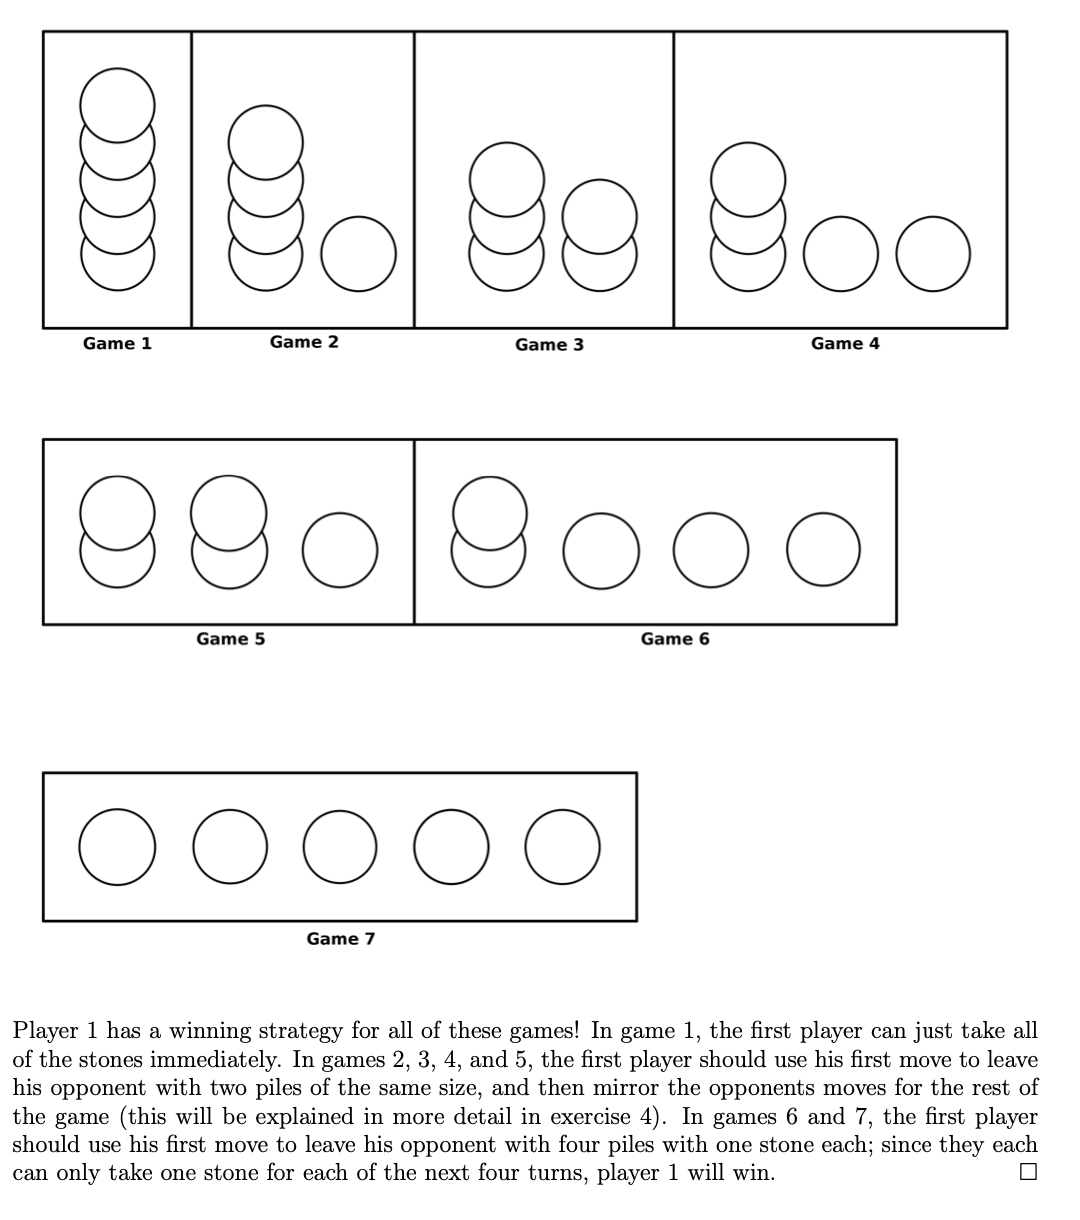
\includegraphics[width=0.5\textwidth]{images/rules.png}
    \caption{Fixed Rules}
    \label{fig:fixed_rules}
\end{figure}


\paragraph{Approach 1: A Lot of If-Elses}
The above rules are applied directly. An if-else sequence decides which strategy to employ based on the current layout and statistics on the nim board.

\begin{mintedbox}{python}
    from collections import Counter
    from copy import deepcopy
    from itertools import accumulate
    import logging
    from operator import xor
    import random
    from typing import Callable

    from lib import Genome, Nim, Nimply


    class FixedRuleNim:
        def __init__(self):
            self.num_moves = 0
            self.OFFSPRING_SIZE = 30
            self.POPULATION_SIZE = 100
            self.GENERATIONS = 100
            self.nim_size = 5

        def nim_sum(self, nim: Nim):
            '''
            Returns the nim sum of the current game board
            by taking an XOR of all the rows.
            Ideally, agent should try to leave nim sum of 0 at the end of turn
            '''
            *_, result = accumulate(nim.rows, xor)
            return result

        def init_population(self, population_size, nim: Nim):
            '''
            Initialize population of genomes,
            key is rule, value is number of sticks to take
            The rules currently are:
            1. If one pile, take $x$ number of sticks from the pile.
            2. If two piles:
                a. If 1 pile has 1 stick, wipe out the pile
                b. If 2 piles have multiple sticks, take x sticks from any pile
            3. If three piles and two piles have the same size, remove all sticks from the smallest pile
            4. If n piles and n-1 piles have the same size, remove x sticks from the smallest pile until it is the same size as the other piles
            '''
            population = []
            for i in range(population_size):
                # rules 3 and 4 are fixed (apply for 3 or more piles)
                # different strategies for different rules (situations on the board)
                individual = {
                    'rule_1': [0, random.randint(0, (nim.num_rows - 1) * 2)],
                    'rule_2a': [random.randint(0, 1), random.randint(0, (nim.num_rows - 1) * 2)],
                    'rule_2b': [random.randint(0, 1), random.randint(0, (nim.num_rows - 1) * 2)],
                    'rule_3': [nim.rows.index(min(nim.rows)), min(nim.rows)],
                    'rule_4': [nim.rows.index(max(nim.rows)), max(nim.rows) - min(nim.rows)]
                }
                genome = Genome(individual)
                population.append(genome)
            return population

        def statistics(self, nim: Nim):
            '''
            Similar to Squillero's cooked function to get possible moves
            and statistics on Nim board
            '''
            # logging.info('In statistics')
            # logging.info(nim.rows)
            stats = {
                'possible_moves': [(r, o) for r, c in enumerate(nim.rows) for o in range(1, c + 1) if nim.k is None or o <= nim.k],
                # 'possible_moves': [(row, num_objects) for row in range(nim.num_rows) for num_objects in range(1, nim.rows[row]+1)],
                'num_active_rows': sum(o > 0 for o in nim.rows),
                'shortest_row': min((x for x in enumerate(nim.rows) if x[1] > 0), key=lambda y: y[1])[0],
                'longest_row': max((x for x in enumerate(nim.rows)), key=lambda y: y[1])[0],
                # only 1-stick row and not all rows having only 1 stick
                '1_stick_row': any([1 for x in nim.rows if x == 1]) and not all([1 for x in nim.rows if x == 1]),
                'nim_sum': self.nim_sum(nim)
            }

            brute_force = []
            for move in stats['possible_moves']:
                tmp = deepcopy(nim)
                tmp.nimming_remove(*move)
                brute_force.append((move, self.nim_sum(tmp)))
            stats['brute_force'] = brute_force

            return stats

        def strategy(self):
            '''
            Returns the best move to make based on the statistics
            '''
            def engine(nim: Nim):
                stats = self.statistics(nim)
                if stats['num_active_rows'] == 1:
                    # logging.info('m1')
                    return Nimply(stats['shortest_row'], random.randint(1, stats['possible_moves'][0][1]))
                elif stats["num_active_rows"] % 2 == 0:
                    # logging.info('m2')
                    if max(nim.rows) == 1:
                        return Nimply(stats['longest_row'], 1)
                    else:
                        pile = random.choice([i for i, x in enumerate(nim.rows) if x > 1])
                        return Nimply(pile, nim.rows[pile] - 1)
                elif stats['num_active_rows'] == 3:
                    # logging.info('m3')
                    unique_elements = set(nim.rows)
                    # check if 2 rows have the same number of sticks
                    two_rows_with_same_elements = False
                    for element in unique_elements:
                        if nim.rows.count(element) == 2:
                            two_rows_with_same_elements = True
                            break

                    if len(nim.rows) == 3 and two_rows_with_same_elements:
                        # remove 1 stick from the longest row
                        logging.info(nim.rows)
                        return Nimply(stats['longest_row'], max(max(nim.rows) - nim.rows[stats['shortest_row']], 1))
                    else:
                        # do something random
                        return Nimply(*random.choice(stats['possible_moves']))
                elif stats['num_active_rows'] >= 4:
                    # logging.info('m4')
                    counter = Counter()
                    for element in nim.rows:
                        counter[element] += 1
                    if len(counter) == 2:
                        if counter.most_common()[0][1] == 1:
                            # remove x sticks from the smallest pile until it is the same size as the other piles
                            return Nimply(stats['shortest_row'], max(nim.rows[stats['shortest_row']] - counter.most_common()[1][0], 1))
                    return random.choice(stats['possible_moves'])
                else:
                    # logging.info('m5')
                    return random.choice(stats['possible_moves'])
            return engine

        def random_agent(self, nim: Nim):
            '''
            Random agent that takes a random move
            '''
            stats = self.statistics(nim)
            return random.choice(stats['possible_moves'])

        def battle(self, opponent, num_games=1000):
            '''
            Battle this agent against another agent
            '''
            wins = 0
            for _ in range(num_games):
                nim = Nim()
                while not nim.goal():
                    nim.nimming_remove(*self.play(nim))
                    if sum(nim.rows) == 0:
                        break
                    nim.nimming_remove(*opponent.play(nim))
                if sum(nim.rows) == 0:
                    wins += 1
            return wins

    if __name__ == '__main__':
        rounds = 20
        evolved_agent_wins = 0
        for i in range(rounds):
            nim = Nim(5)
            orig = nim.rows
            fixedrule = FixedRuleNim()
            engine = fixedrule.strategy()

            # play against random
            player = 0
            while not nim.goal():
                if player == 0:
                    move = engine(nim)
                    logging.info('move of player 1: ', move)
                    nim.nimming_remove(*move)
                    player = 1
                    logging.info("After Player 1 made move: ", nim.rows)
                else:
                    move = fixedrule.random_agent(nim)
                    logging.info('move of player 2: ', move)
                    nim.nimming_remove(*move)
                    player = 0
                    logging.info("After Player 2 made move: ", nim.rows)
            winner = 1 - player
            if winner == 0:
                evolved_agent_wins += 1
        logging.info(f'Fixed rule agent won {evolved_agent_wins} out of {rounds} games')
\end{mintedbox}

\paragraph{Approach 2: Nim-Sum} Will always win
\begin{mintedbox}{python}
from copy import deepcopy
from itertools import accumulate
from operator import xor
import random
import logging
from lib import Nim

# 3.1: Agent Using Fixed Rules
class ExpertNimSumAgent:
    '''
    Play the game of Nim using a fixed rule
    (always leave nim-sum at the end of turn)
    '''
    def __init__(self):
        self.num_moves = 0

    def nim_sum(self, nim: Nim):
        '''
        Returns the nim sum of the current game board
        by taking an XOR of all the rows.
        Ideally, agent should try to leave nim sum of 0 at the end of turn
        '''
        *_, result = accumulate(nim.rows, xor)
        return result
        # return sum([i^r for i, r in enumerate(nim._rows)])

    def play(self, nim: Nim):
        # remove objects from row to make nim-sum 0
        nim_sum = self.nim_sum(nim)
        all_possible_moves = [(r, o) for r, c in enumerate(nim.rows) for o in range(1, c+1)]
        move_found = False
        for move in all_possible_moves:
            replicated_nim = deepcopy(nim)
            replicated_nim.nimming_remove(*move)
            if self.nim_sum(replicated_nim) == 0:
                nim.nimming_remove(*move)
                move_found = True
                break
        # if a valid move not found, return random move
        if not move_found:
            move = random.choice(all_possible_moves)
            nim.nimming_remove(*move)

        # logging.info(f"Move {self.num_moves}: Removed {move[1]} objects from row {move[0]}")
        self.num_moves += 1
\end{mintedbox}

\subsubsection{Evolved Agent Approach 1}

The rules are evolved using a genetic algorithm. A dictionary of strategies is evolved. The key is the rule (scenario/antecedent). The value is the maximum number of sticks to leave on the board in this scenario.

For instance, for rule 1, the value tuned is the
 in "If one pile, leave a max of x sticks in the pile".

\begin{markdown}
    rule_strategy = {
        "one_pile": 2,
        "two_piles": 3,
        "three_piles": 3,
        "n_piles": 4
    }

    # after mutation / crossover
    rule_strategy = {
        "one_pile": 3,
        "two_piles": 2,
        "three_piles": 3,
        "n_piles": 4
    }

\end{markdown}

Mutation essentially swaps the values in the dictionaries. Crossover takes two parents and randomly chooses strategies for different rules. Intuitively, the machine tries to learn the best strategy for each scenario on the board.

\begin{table}
\centering
\begin{tabular}{|c|c|c|}
\hline
Opponent 1 & Opponent 2 & Win Rate \\ \hline
Evolved & Random & 70\% \\ \hline
\end{tabular}
\end{table}

\begin{mintedbox}{python}
    '''
In this file, I will try to implement Nim where there is an evolved set of rules/strategies.
For each scenario, I will have a set of rules that will be used to determine the best move.
They are obtained from discussion with friends and from the paper "The Game of Nim" by Ryan Julian
The rules currently are:
1. If one pile, take $x$ number of sticks from the pile.
2. If two piles:
    a. If 1 pile has 1 stick, take x sticks
    b. If 2 piles have multiple sticks, take x sticks from the larger pile
3. If three piles and two piles have the same size, remove all sticks from the smallest pile
4. If n piles and n-1 piles have the same size, remove x sticks from the smallest pile until it is the same size as the other piles
'''

from collections import Counter, namedtuple
from copy import deepcopy
from itertools import accumulate
import logging
from operator import xor
import random
from typing import Callable

from lib import Genome, Nim, Nimply

class BrilliantEvolvedAgent:
    def __init__(self):
        self.num_moves = 0
        self.OFFSPRING_SIZE = 200
        self.POPULATION_SIZE = 50
        self.GENERATIONS = 100
        self.nim_size = 5

    def nim_sum(self, nim: Nim):
        '''
        Returns the nim sum of the current game board
        by taking an XOR of all the rows.
        Ideally, agent should try to leave nim sum of 0 at the end of turn
        '''
        *_, result = accumulate(nim.rows, xor)
        return result

    def init_population(self, population_size, nim: Nim):
        '''
        Initialize population of genomes,
        key is rule, value is number of sticks to take
        The rules currently are:
        1. If one pile, take $x$ number of sticks from the pile.
        2. If two piles:
            a. If 1 pile has 1 stick, wipe out the pile
            b. If 2 piles have multiple sticks, take x sticks from any pile
        3. If three piles and two piles have the same size, remove all sticks from the smallest pile
        4. If n piles and n-1 piles have the same size, remove x sticks from the smallest pile until it is the same size as the other piles
        5. If none of the above rules apply, just pick a random pile and take a random number of sticks
        '''
        population = []
        for i in range(population_size):
            # rules 3 and 4 are fixed (apply for 3 or more piles)
            # different strategies for different rules (situations on the board)
            individual = {
                'rule_1': [0, random.randint(0, (self.nim_size - 1) * 2)],
                'rule_2a': [random.randint(0, 1), random.randint(0, (self.nim_size - 1) * 2)],
                'rule_2b': [random.randint(0, 1), random.randint(0, (self.nim_size - 1) * 2)],
                'rule_3': [nim.rows.index(min(nim.rows)), min(nim.rows)],
                'rule_4': [nim.rows.index(max(nim.rows)), max(nim.rows) - min(nim.rows)]
            }
            genome = Genome(individual)
            population.append(genome)
        return population

    def crossover(self, parent1, parent2, crossover_rate):
        '''
        Crossover function to combine two parents into a child
        '''
        child = {}
        for rule in parent1.rules:
            if random.random() < crossover_rate:
                child[rule] = parent1.rules[rule]
            else:
                child[rule] = parent2.rules[rule]
        return Genome(child)

    def tournament_selection(self, population, tournament_size):
        '''
        Tournament selection to select the best genomes
        '''
        tournament = random.sample(population, tournament_size)
        tournament.sort(key=lambda x: x.fitness, reverse=True)
        return tournament[0]

    def mutate(self, genome: Genome, mutation_rate=0.5):
        '''
        Mutate the genome by switching one of the rules (can end up in something stupid like removing more sticks than there are, but this is checked in the strategy function)
        '''
        rule = random.choice(list(genome.rules.keys()))
        # swap some keys
        if rule == 'rule_1':
            genome.rules[rule] = [0, random.randint(0, (self.nim_size - 1) * 2)]
        elif rule == 'rule_2a':
            genome.rules[rule] = [random.randint(0, 1), random.randint(0, (self.nim_size - 1) * 2)]
        elif rule == 'rule_2b':
            genome.rules[rule] = [random.randint(0, 1), random.randint(0, (self.nim_size - 1) * 2)]
        elif rule == 'rule_3':
            genome.rules[rule] = [random.randint(0, self.nim_size - 1), random.randint(0, (self.nim_size - 1) * 2)]
        elif rule == 'rule_4':
            genome.rules[rule] = [random.randint(0, self.nim_size - 1), random.randint(0, (self.nim_size - 1) * 2)]
        return genome
        # rule = random.choice(list(genome.rules.keys()))
        # if random.random() < mutation_rate:
        #     genome.rules[rule] = [random.randint(0, 1), random.randint(0, self.nim_size * 2)]
        # return genome
        # rule = random.choice(list(genome.keys()))
        # genome[rule] = random.randint(1, 10)

    def statistics(self, nim: Nim):
        '''
        Similar to Squillero's cooked function to get possible moves
        and statistics on Nim board
        '''
        stats = {
            'possible_moves': [(r, o) for r, c in enumerate(nim.rows) for o in range(1, c + 1) if nim.k is None or o <= nim.k],
            # 'possible_moves': [(row, num_objects) for row in range(nim.num_rows) for num_objects in range(1, nim.rows[row]+1)],
            'num_active_rows': sum(o > 0 for o in nim.rows),
            'shortest_row': min((x for x in enumerate(nim.rows) if x[1] > 0), key=lambda y: y[1])[0],
            'longest_row': max((x for x in enumerate(nim.rows)), key=lambda y: y[1])[0],
            # only 1-stick row and not all rows having only 1 stick
            '1_stick_row': any([1 for x in nim.rows if x == 1]) and not all([1 for x in nim.rows if x == 1]),
            'nim_sum': self.nim_sum(nim)
        }

        brute_force = []
        for move in stats['possible_moves']:
            tmp = deepcopy(nim)
            tmp.nimming_remove(*move)
            brute_force.append((move, self.nim_sum(tmp)))
        stats['brute_force'] = brute_force

        return stats

    def strategy(self, genome: dict):
        '''
        Returns the best move to make based on the statistics
        '''
        def evolution(nim: Nim):
            stats = self.statistics(nim)
            if stats['num_active_rows'] == 1:
                num_to_leave = genome.rules['rule_1'][1]
                # see which move will leave the most sticks
                most_destructive_move = max(stats['possible_moves'], key=lambda x: x[1])
                if num_to_leave >= most_destructive_move[1]:
                    # remove only 1 stick
                    return Nimply(most_destructive_move[0], 1)
                else:
                    # make the move that leaves the desired number of sticks
                    move = [(row, num_objects) for row, num_objects in stats['possible_moves'] if nim.rows[row] - num_objects == num_to_leave]
                    if len(move) > 0:
                        return Nimply(*move[0])
                    else:
                        # make random move
                        return Nimply(*random.choice(stats['possible_moves']))

            elif stats['num_active_rows'] == 2:
                # rule 2a
                if stats['1_stick_row']:
                    # if there is a 1-stick row, have to choose between wiping it out or taking from the other row
                    if genome.rules['rule_2a'][0] == 0:
                        # wipe out the 1-stick row
                        logging.info('wiping out 1-stick row')
                        pile = [row for row in range(nim.num_rows) if nim.rows[row] == 1][0]
                        return Nimply(pile, 1)
                    else:
                        # take out the desired number of sticks from the other row
                        pile = random.choice([index for index, x in enumerate(nim.rows) if x > 1])
                        num_objects_to_remove = max(1, nim.rows[pile] - genome.rules['rule_2a'][1])
                        # move = [(row, num_objects) for row, num_objects in stats['possible_moves'] if nim.rows[row] - num_objects == genome.rules['rule_2a'][1]]
                        return Nimply(pile, num_objects_to_remove)
                # rule 2b
                # both piles have many elements, take from either the smallest or the largest pile
                else:
                    if genome.rules['rule_2b'][0] == 0:
                        # take from the smallest pile
                        pile = stats['shortest_row']
                        num_objects_to_remove = max(1, nim.rows[pile] - genome.rules['rule_2b'][1])
                        return Nimply(pile, num_objects_to_remove)
                    else:
                        # take from the largest pile
                        pile = stats['longest_row']
                        num_objects_to_remove = max(1, nim.rows[pile] - genome.rules['rule_2b'][1])
                        return Nimply(pile, num_objects_to_remove)

            elif stats['num_active_rows'] == 3:
                unique_elements = set(nim.rows)
                # check if 2 rows have the same number of sticks
                two_rows_with_same_elements = False
                for element in unique_elements:
                    if nim.rows.count(element) == 2:
                        two_rows_with_same_elements = True
                        break

                if len(nim.rows) == 3 and two_rows_with_same_elements:
                    # remove 1 stick from the longest row
                    return Nimply(stats['longest_row'], max(max(nim.rows) - nim.rows[stats['shortest_row']], 1))
                else:
                    # do something random
                    return Nimply(*random.choice(stats['possible_moves']))

            counter = Counter()
            for element in nim.rows:
                counter[element] += 1
            if len(counter) == 2:
                if counter.most_common()[0][1] == 1:
                    # remove x sticks from the smallest pile until it is the same size as the other piles
                    return Nimply(stats['shortest_row'], max(nim.rows[stats['shortest_row']] - counter.most_common()[1][0], 1))
                # else:
                #     return random.choice(stats['possible_moves'])

            # for large number of piles, general rule to remove all but 1 stick from a random pile
            if stats["num_active_rows"] % 2 == 0:
                if nim.rows[stats['longest_row']] == 1:
                    return Nimply(stats['longest_row'], 1)
                else:
                    pile = random.choice([i for i, x in enumerate(nim.rows) if x > 1])
                    return Nimply(pile, nim.rows[pile] - 1)

            else:
                # this is a fixed rule, does not have random component
                # rule from the paper Ryan Julian: The Game of Nim
                # If n piles and n-1 piles have the same size, remove x sticks from the smallest pile until it is the same size as the other piles
                # check if only 1 pile has a different number of sticks
                # just make a random move if all else fails
                return random.choice(stats['possible_moves'])
        return evolution

    def random_agent(self, nim: Nim):
        '''
        Random agent that takes a random move
        '''
        stats = self.statistics(nim)
        return random.choice(stats['possible_moves'])

    def dumb_agent(self, nim: Nim):
        '''
        Agent that takes one element from the longest row
        '''
        stats = self.statistics(nim)
        return (stats['longest_row'], 1)

    def aggressive_agent(self, nim: Nim):
        '''
        Agent that takes the largest possible move
        '''
        stats = self.statistics(nim)
        if stats['num_active_rows'] % 2 == 0:
            return random.choice(stats['possible_moves'])
        else:
            row = stats['longest_row']
            return (row, nim.rows[row])

        # stats = self.statistics(nim)
        # return max(stats['possible_moves'], key=lambda x: x[1])

    def calculate_fitness(self, genome):
        '''
        Calculate fitness by playing the genome's strategy against a random agent
        (cannot use nim sum agent as it is too good)
        '''
        wins = 0
        for i in range(5):
            nim = Nim(5)
            player = 0
            engine = self.strategy(genome)
            while not nim.goal():
                if player == 0:
                    move = engine(nim)
                    nim.nimming_remove(*move)
                    player = 1
                else:
                    nim.nimming_remove(*self.random_agent(nim))
                    player = 0
            winner = 1 - player
            if winner == 0:
                wins += 1
        return wins / 5

    def select_survivors(self, population: list, num_survivors: int):
        '''
        Select the best genomes from the population
        '''
        return sorted(population, key=lambda x: x.fitness, reverse=True)[:num_survivors]

    def learn(self, population_size=100, mutation_rate=0.1, crossover_rate=0.7, nim: Nim = None):
        initial_population = self.init_population(population_size, nim)
        for genome in initial_population:
            genome.fitness = self.calculate_fitness(genome)
        for i in range(self.GENERATIONS):
            # logging.info(f'Generation {i}')
            new_offspring = []
            for j in range(self.OFFSPRING_SIZE):
                parent1 = random.choice(initial_population)
                parent2 = random.choice(initial_population)
                child = self.crossover(parent1, parent2, crossover_rate)
                child = self.mutate(child)
                new_offspring.append(child)
            initial_population += new_offspring
            initial_population = self.select_survivors(initial_population, population_size)
        best_strategy = initial_population[0]
        return best_strategy

    def battle(self, opponent, num_games=1000):
        '''
        Battle this agent against another agent
        '''
        wins = 0
        for _ in range(num_games):
            nim = Nim()
            while not nim.goal():
                nim.nimming_remove(*self.play(nim))
                if sum(nim.rows) == 0:
                    break
                nim.nimming_remove(*opponent.play(nim))
            if sum(nim.rows) == 0:
                wins += 1
        return wins

if __name__ == '__main__':
    rounds = 20
    evolved_agent_wins = 0
    for i in range(rounds):
        nim = Nim(5)
        orig = nim.rows
        brilliantagent = BrilliantEvolvedAgent()
        best_strategy = brilliantagent.learn(nim=nim)
        engine = brilliantagent.strategy(best_strategy)

        # play against random
        player = 0
        while not nim.goal():
            if player == 0:
                move = engine(nim)
                logging.info('move of player 1: ', move)
                nim.nimming_remove(*move)
                player = 1
                logging.info("After Player 1 made move: ", nim.rows)
            else:
                move = brilliantagent.random_agent(nim)
                logging.info('move of player 2: ', move)
                nim.nimming_remove(*move)
                player = 0
                logging.info("After Player 2 made move: ", nim.rows)
        winner = 1 - player
        if winner == 0:
            evolved_agent_wins += 1
    logging.info(f'Evolved agent won {evolved_agent_wins} out of {rounds} games')
\end{mintedbox}

\subsubsection{Evolved Agent Approach 2 (Probability Thresholds)}

Strategies were originally chosen based on probability thresholds and a random number. The list of probabilities (thresholds) are evolved using a genetic algorithm. \emph{Intuitively, the machine tries to learn the best probability of choosing each strategy, regardless of the rule.}

\begin{mintedbox}{python}
    thresholds = [p1, p2, p3]
    if random.random() < p1:
        # strategy 1...
    elif random.random() < p2:
        # strategy 2...
    else:
        # strategy 3...

    class GA:
        ...

    GA.evolve(thresholds)
\end{mintedbox}

I discussed this approach with both Prof. Squillero and Calabrese. They both agreed that this was worth exploring. However, upon implementing, I realised that tuning probability thresholds produces poor, near-random performance, \emph{as the system is making decisions without any knowledge of the current situation on the board, or any knowledge of the rules}.

\begin{mintedbox}{python}
    # 3.2: Agent Using Evolved Rules (Randomly Chooses Between Strategies Based on Probabilities)
    from itertools import accumulate
    from operator import xor
    import random
    import numpy as np

    from lib import Nim

    class EvolvedAgent1:
        '''
        Plays Nim using a set of rules that are evolved
        '''
        def __init__(self):
            self.num_moves = 0

        def nim_sum(self, nim: Nim):
            '''
            Returns the nim sum of the current game board
            by taking an XOR of all the rows.
            Ideally, agent should try to leave nim sum of 0 at the end of turn
            '''
            *_, result = accumulate(nim.rows, xor)
            return result

        def play_nim(self, nim: Nim, prob_list: list):
            '''
            GA can choose between the following strategies:
            1. Randomly pick any row and any number of elements from that row
            2. Pick the shortest row
            3. Pick the longest row
            4. Pick based on the nim-sum of the current game board
            '''
            all_possible_moves = [(r, o) for r, c in enumerate(nim.rows) for o in range(1, c+1)]
            strategies = {
                'nim_sum': random.choice([move for move in all_possible_moves if self.nim_sum(deepcopy(nim).nimming_remove(*move)) == 0]),
                'random': random.choice(all_possible_moves),
                'all_elements_shortest_row': (nim.rows.index(min(nim.rows)), min(nim.rows)),
                '1_element_shortest_row': (nim.rows.index(min(nim.rows)), 1),
                'random_element_shortest_row': (nim.rows.index(min(nim.rows)), random.randint(1, min(nim.rows))),
                'all_elements_longest_row': (nim.rows.index(max(nim.rows)), max(nim.rows)),
                '1_element_longest_row': (nim.rows.index(max(nim.rows)), 1),
                'random_element_longest_row': (nim.rows.index(max(nim.rows)), random.randint(1, max(nim.rows))),
            }

            p = random.random()
            strategy = None
            if p < prob_list[0]:
                strategy = strategies['random']
            elif p >= prob_list[0] and p < prob_list[1]:
                strategy = random.choice([strategies['all_elements_shortest_row'], strategies['1_element_shortest_row'], strategies['random_element_shortest_row']])
            elif p >= prob_list[1] and p < prob_list[2]:
                strategy = random.choice([strategies['all_elements_longest_row'], strategies['1_element_longest_row'], strategies['random_element_longest_row']])
            else:
                strategy = strategies['nim_sum']

            nim.nimming_remove(*strategy)
            self.num_moves += 1
            return sum(nim.rows)

        def play(self, nim: Nim):
            '''
            Play the game of Nim using the evolved rules
            '''
            prob_list = [0.25, 0.5, 0.75, 1]
            prob_list = self.evolve_probabilities(nim, prob_list, 20, 5)
            self.play_nim(nim, prob_list)

        def crossover(self, p1, p2):
            '''
            Crossover between two parents
            '''
            return np.random.choice(p1 + p2, size=4, replace=True)

        def evolve_probabilities(self, nim: Nim, prob_list: list, num_generations: int, num_children: int):
            '''
            Evolve the probabilities of the strategies
            '''
            # create initial population
            population = [prob_list for _ in range(num_children)]
            # create initial fitness scores
            fitness_scores = [self.play(nim, p) for p in population]
            # create initial parents
            parents = [population[i] for i in np.argsort(fitness_scores)[:2]]
            # create new population
            new_population = []
            for _ in range(num_generations):
                # create children
                for _ in range(num_children):
                    p1 = random.choice(parents)
                    p2 = random.choice(parents)
                    child = self.crossover(p1, p2)
                    # child = []
                    # for i in range(len(parents[0])):
                    #     # crossover between parents

                    #     child.append(random.choice(parents)[i])
                    new_population.append(child)
                # create fitness scores
                fitness_scores = [self.play_nim(nim, p) for p in new_population]
                # create new parents
                parents = [new_population[i] for i in np.argsort(fitness_scores)[:2]]
                # create new population
                new_population = []
            return parents[0]
\end{mintedbox}

\subsubsection{Minmax}

In `minmax.py`, the minimax algorithm is implemented. It recursively traverses the game tree to maximise potential returns. As a result, it is a near-optimal strategy that reported `100\%` win rate against random opponents.

Since the recursive algorithm is slow:

\begin{enumerate}
    \item The tree is pruned momentarily, stopping the algorithm from exploring parts of the tree that will not materialise on the game board.
    \item A maximum depth is set, so that the recursive loop is stopped when a particular depth is reached.
\end{enumerate}

Although not significant, an `@lru\_cache` decorator is applied on the minmax operation after ensuring that the Nim state (row composition) is serializable.

\begin{mintedbox}{python}
from copy import deepcopy
from functools import lru_cache
from itertools import accumulate
import math
from operator import xor
from evolved_nim import BrilliantEvolvedAgent
import logging
from lib import Nim

logging.basicConfig(level=logging.INFO)

class MinMaxAgent:
    def __init__(self):
        self.num_moves = 0

    def nim_sum(self, nim: Nim):
        '''
        Returns the nim sum of the current game board
        by taking an XOR of all the rows.
        Ideally, agent should try to leave nim sum of 0 at the end of turn
        '''
        *_, result = accumulate(nim.rows, xor)
        return result

    def evaluate(self, nim: Nim, is_maximizing: bool):
        '''
        Returns the evaluation of the current game board
        '''
        if all(row == 0 for row in nim.rows):
            return -1 if is_maximizing else 1
        else:
            return -1

    @lru_cache(maxsize=1000)
    def minmax(self, nim: Nim, depth: int, maximizing_player: bool, alpha: int = -1, beta: int = 1, max_depth: int = 7):
        '''
        Depth-limited Minimax algorithm to find the best move with alpha-beta pruning and depth limit
        '''
        logging.info("Depth ", depth)
        if depth == 0 or nim.goal() or depth == max_depth:
            # logging.info("Depth ", depth)
            # logging.info("Nim goal ", nim.goal())
            return self.evaluate(nim, maximizing_player)

        if maximizing_player:
            value = -math.inf
            for r, c in enumerate(nim.rows):
                for o in range(1, c+1):
                    # make copy of nim object before running a nimming operation
                    replicated_nim = deepcopy(nim)
                    replicated_nim.nimming_remove(r, o)
                    value = max(value, self.minmax(replicated_nim, depth-1, False, alpha, beta))
                    alpha = max(alpha, value)
                    if beta <= alpha:
                        logging.info("Pruned")
                        break
            return value
        else:
            value = math.inf
            for r, c in enumerate(nim.rows):
                for o in range(1, c+1):
                    # make copy of nim object before running a nimming operation
                    replicated_nim = deepcopy(nim)
                    replicated_nim.nimming_remove(r, o)
                    value = min(value, self.minmax(replicated_nim, depth-1, True, alpha, beta))
                    beta = min(beta, value)
                    if beta <= alpha:
                        logging.info("Pruned")
                        break
            return value

    def play(self, nim: Nim):
        '''
        Agent returns the best move based on minimax algorithm
        '''
        possible_moves = []
        for r, c in enumerate(nim.rows):
            for o in range(1, c+1):
                # make copy of nim object before running a nimming operation
                replicated_nim = deepcopy(nim)
                replicated_nim.nimming_remove(r, o)
                possible_moves.append((r, o, self.minmax(replicated_nim, 10, False)))
        # sort possible moves by the value returned by minimax
        possible_moves.sort(key=lambda x: x[2], reverse=True)
        # return the best move
        return possible_moves[0][0], possible_moves[0][1]

    def battle(self, opponent, num_games=1000):
        '''
        Battle this agent against another agent
        '''
        wins = 0
        for _ in range(num_games):
            nim = Nim()
            while not nim.goal():
                nim.nimming_remove(*self.play(nim))
                if sum(nim.rows) == 0:
                    break
                nim.nimming_remove(*opponent.play(nim))
            if sum(nim.rows) == 0:
                wins += 1
        return wins

if __name__ == "__main__":

    rounds = 10

    minmax_wins = 0
    for i in range(rounds):
        nim = Nim(num_rows=5)
        agent = MinMaxAgent()
        random_agent = BrilliantEvolvedAgent()
        player = 0
        while not nim.goal():
            if player == 0:
                move = agent.play(nim)
                logging.info(f"Minmax move {agent.num_moves}: Removed {move[1]} objects from row {move[0]}")
                logging.info(nim.rows)
                nim.nimming_remove(*move)
            else:
                move = random_agent.random_agent(nim)
                logging.info(f"Random move {random_agent.num_moves}: Removed {move[1]} objects from row {move[0]}")
                logging.info(nim.rows)
                nim.nimming_remove(*move)
            player = 1 - player

        winner = 1 - player
        if winner == 0:
            minmax_wins += 1
        # player that made the last move wins
        logging.info(f"Player {winner} wins in round {i+1}!")

    logging.info(f"Minmax wins {minmax_wins} out of {rounds} rounds")
\end{mintedbox}

\subsubsection{Reinforcement Learning}

Both temporal difference learning (TDL) and monte carlo learning (MCL) are implemented. In TDL, the Q values are updated after each move. In MCL, the learning is episodic so a goal dictionary is traversed backwards. \\

\paragraph{State Hashing} The state for TDL consists of a key-value dictionary. The representation is: (the rows in nim, action tuple): Q. The rows are hashed into a string, with each value separated by a hyphen. In TDL, Q values are updated after each move.

\paragraph{Temporal Difference Learning (TDL)}

\begin{equation*}
    Q(s, a) \leftarrow Q(s, a) + \alpha \left( r + \gamma \max_{a'} Q(s', a') - Q(s, a) \right)
\end{equation*}

TDL exploits the Markov property of the game, where the next state is only dependent on the current state and the action taken. Performance was initially poor, but improved after tuning the hyperparameters (alpha, gamma, epsilon).

The best reported win rate is 80\% against a random opponent after 5000 rounds of training at a 0.4 epsilon (exploration rate) and 1000 iterations of testing at 0 epsilon (max exploitation). Learning rate is decayed accordingly.

\begin{mintedbox}{python}
class NimRLTemporalDifferenceAgent:
"""
An agent that learns to play Nim through temporal difference learning.
"""
def __init__(self, num_rows: int, epsilon: float = 0.4, alpha: float = 0.3, gamma: float = 0.9):
    """Initialize agent."""
    self.num_rows = num_rows
    self.epsilon = epsilon
    self.alpha = alpha
    self.gamma = gamma
    self.current_state = None
    self.previous_state = None
    self.previous_action = None
    self.Q = dict()

def init_reward(self, state: Nim):
    '''Initialize reward for every state and every action with a random value'''
    for i in range(1, state.num_rows):
        nim = Nim(num_rows=i)
        for r, c in enumerate(nim.rows):
            for o in range(1, c+1):
                self.set_Q(hash_list(nim.rows), (r, o),
                            np.random.uniform(0, 0.01))

def get_Q(self, state: Nim, action: tuple):
    """Return Q-value for state and action."""
    if (hash_list(state.rows), action) in self.Q:
        logging.info("Getting Q for state: {} and action: {}".format(hash_list(state.rows), action))
        logging.info("Q-value: {}".format(self.Q[(hash_list(state.rows), action)]))
        return self.Q[(hash_list(state.rows), action)]
    else:
        # initialize Q-value for state and action
        self.set_Q(hash_list(state.rows), action, np.random.uniform(0, 0.01))
        return self.Q[(hash_list(state.rows), action)]

def set_Q(self, state: str, action: tuple, value: float):
    """Set Q-value for state and action."""
    # logging.info("Setting Q for state: {} and action: {} to value: {}".format(state, action, value))
    self.Q[(state, action)] = value

def get_max_Q(self, state: Nim):
    """Return maximum Q-value for state."""
    max_Q = -math.inf
    # logging.info(state.rows)
    for r, c in enumerate(state.rows):
        for o in range(1, c+1):
            # logging.info("Just Q: {}".format(self.get_Q(state, (r, o))))
            max_Q = max(max_Q, self.get_Q(state, (r, o)))
    # logging.info("Max Q: {}".format(max_Q))
    return max_Q

def get_average_Q(self, state: Nim):
    """Return average Q-value for state."""
    total_Q = 0
    for r, c in enumerate(state.rows):
        for o in range(1, c+1):
            total_Q += self.get_Q(state, (r, o))
    return total_Q / len(state.rows)

def get_possible_actions(self, state: Nim):
    """Return all possible actions for state."""
    possible_actions = []
    for r, c in enumerate(state.rows):
        for o in range(1, c+1):
            possible_actions.append((r, o))
    return possible_actions

def get_action(self, state: Nim):
    """Return action based on epsilon-greedy policy."""
    if random.random() < self.epsilon:
        return random.choice(self.get_possible_actions(state))
    else:
        logging.info("Getting best action")
        max_Q = -math.inf
        best_action = None
        for r, c in enumerate(state.rows):
            for o in range(1, c+1):
                Q = self.get_Q(state, (r, o))
                if Q > max_Q:
                    max_Q = Q
                    best_action = (r, o)
        return best_action

def register_state(self, state: Nim):
    # for each possible move in state, initialize random Q value
    for r, c in enumerate(state.rows):
        for o in range(1, c+1):
            if (hash_list(state.rows), (r, o)) not in self.Q:
                val = np.random.uniform(0, 0.01)
                # logging.info("Registering state: {} and action: {} to {}".format(state.rows, (r, o), val))
                self.set_Q(hash_list(state.rows), (r, o), val)
            else:
                logging.info("State already registered: {} and action: {}".format(state.rows, (r, o)))

def update_Q(self, reward: int, game_over: bool):
    """Update Q-value for previous state and action."""

    if game_over:
        # self.set_Q(hash_list(self.previous_state.rows), self.previous_action, reward)
        self.set_Q(hash_list(self.previous_state.rows), self.previous_action, self.get_Q(self.previous_state, self.previous_action) + self.alpha * (reward - self.get_Q(self.previous_state, self.previous_action)))

    else:
    # if reward != -1:
        self.register_state(self.current_state)
        if self.previous_action is not None:
            self.set_Q(hash_list(self.previous_state.rows), self.previous_action, self.get_Q(self.previous_state, self.previous_action) +
                        self.alpha * (reward + self.gamma) * (self.get_max_Q(self.current_state) - self.get_Q(self.previous_state, self.previous_action)))
    # else:
    #     self.set_Q(hash_list(self.previous_state.rows), self.previous_action, self.get_Q(self.previous_state, self.previous_action) + self.alpha * (reward - self.get_Q(self.previous_state, self.previous_action)))

def print_best_action_for_each_state(self):
    for state in self.Q:
        logging.info("State: {}".format(state[0]))
        nim = Nim(5)
        nim.rows = unhash_list(state[0])
        logging.info("Best action: {}".format(self.choose_action(nim)))

def test_against_random(self, round, random_agent):
    wins = 0
    for i in range(rounds):
        nim = Nim(num_rows=5)
        player = 0
        while not nim.goal():
            if player == 0:
                move = self.choose_action(nim)
                # logging.info(f"Reinforcement move: Removed {move[1]} objects from row {move[0]}")
                nim.nimming_remove(*move)
            else:
                move = random_agent(nim)
                # logging.info(f"Random move {random_agent.num_moves}: Removed {move[1]} objects from row {move[0]}")
                nim.nimming_remove(*move)
            player = 1 - player

        winner = 1 - player
        if winner == 0:
            wins += 1

    logging.info(f"Win Rate in round {round}: {wins / rounds}")

def battle(self, agent, rounds=1000, training=True, momentary_testing=False):
    """Train agent by playing against other agents."""
    agent_wins = 0
    winners = []
    for episode in range(rounds):
        # logging.info(f"Episode {episode}")
        nim = Nim(num_rows=5)
        self.current_state = nim
        self.previous_state = None
        self.previous_action = None
        player = 0
        while True:
            reward = 0
            if player == 0:
                self.previous_state = deepcopy(self.current_state)
                self.previous_action = self.get_action(self.current_state)
                self.current_state.nimming_remove(
                    *self.previous_action)
                player = 1
            else:
                move = agent(self.current_state)
                # logging.info("Random agent move: {}".format(move))
                self.current_state.nimming_remove(*move)
                player = 0

            # learning by calculating reward for the current state
            if self.current_state.goal():
                winner = 1 - player
                if winner == 0:
                    logging.info("Agent won")
                    agent_wins += 1
                    reward = 1
                else:
                    logging.info("Random won")
                    reward = -1
                winners.append(winner)
                self.update_Q(reward, self.current_state.goal())
                break
            else:
                self.update_Q(reward, self.current_state.goal())

        # decay epsilon after each episode
        self.epsilon = self.epsilon - 0.1 if self.epsilon > 0.1 else 0.1
        self.alpha *= -0.0005
        if self.alpha < 0.1:
            self.alpha = 0.1

        if training and momentary_testing:
            if episode % 100 == 0:
                logging.info(f"Episode {episode} finished, sampling")
                random_agent = BrilliantEvolvedAgent()
                self.test_against_random(
                    episode, random_agent.random_agent)

    if not training:
        logging.info("Reinforcement agent won {} out of {} games".format(
            agent_wins, rounds))
    # self.print_best_action_for_each_state()
    return winners

def choose_action(self, state: Nim):
    """Return action based on greedy policy."""
    max_Q = -math.inf
    best_action = None
    for r, c in enumerate(state.rows):
        for o in range(1, c+1):
            Q = self.get_Q(state, (r, o))
            if Q > max_Q:
                max_Q = Q
                best_action = (r, o)
    if best_action is None:
        return random.choice(self.get_possible_actions(state))
    else:
        return best_action

if __name__ == "__main__":
rounds = 10000
minmax_wins = 0

nim = Nim(num_rows=5)
agent_tda = NimRLTemporalDifferenceAgent(num_rows=5)
random_agent = RandomAgent()

# agentG = NimRLMonteCarloAgent(num_rows=7)
agent_tda.battle(random_agent.play, rounds=10000)
agent_tda.epsilon = 0.1

# TESTING
logging.info("Testing against random agent")
agent_tda.battle(random_agent.random_agent, training=False, rounds=1000)
\end{mintedbox}

\paragraph{Monte Carlo Learning}

\begin{equation*}
    Q(s, a) \leftarrow Q(s, a) + \alpha \left( G - Q(s, a) \right)
\end{equation*}

In MCL, the learning is episodic so a goal dictionary is traversed backwards. MCL takes a more holistic approach to learning, where rewards are based on every past move.

\begin{mintedbox}{python}
logging.basicConfig(level=logging.INFO)

def hash_list(l):
    '''
    Hashes a list of integers into a string
    '''
    return "-".join([str(i) for i in l])


def unhash_list(l):
    '''
    Unhashes a string of integers into a list
    '''
    return [int(i) for i in l.split("-")]


def decay(value, decay_rate):
    return value * decay_rate


class NimRLMonteCarloAgent:
    def __init__(self, num_rows: int, epsilon: float = 0.3, alpha: float = 0.5, gamma: float = 0.9):
        """Initialize agent."""
        self.num_rows = num_rows
        self.epsilon = epsilon
        self.alpha = alpha
        self.gamma = gamma
        self.current_state = None
        self.previous_state = None
        self.previous_action = None
        self.G = dict()
        self.state_history = []

    def get_action(self, state: Nim):
        """Return action based on epsilon-greedy policy."""
        if random.random() < self.epsilon:
            action = random.choice(self.get_possible_actions(state))
            if (hash_list(state.rows), action) not in self.G:
                self.G[(hash_list(state.rows), action)] = random.uniform(1.0, 0.01)
            return action
        else:
            max_G = -math.inf
            best_action = None
            for r, c in enumerate(state.rows):
                for o in range(1, c+1):
                    if (hash_list(state.rows), (r, o)) not in self.G:
                        self.G[(hash_list(state.rows), (r, o))] = random.uniform(1.0, 0.01)
                        G = self.G[(hash_list(state.rows), (r, o))]
                    else:
                        G = self.G[(hash_list(state.rows), (r, o))]
                    if G > max_G:
                        max_G = G
                        best_action = (r, o)
            return best_action

    def update_state(self, state, reward):
        self.state_history.append((state, reward))

    def learn(self):
        target = 0

        for state, reward in reversed(self.state_history):
            self.G[state] = self.G.get(state, 0) + self.alpha * (target - self.G.get(state, 0))
            target += reward

        self.state_history = []
        self.epsilon -= 10e-5

    def compute_reward(self, state: Nim):
        return 0 if state.goal() else -1

    def get_possible_actions(self, state: Nim):
        actions = []
        for r, c in enumerate(state.rows):
            for o in range(1, c+1):
                actions.append((r, o))
        return actions

    def get_G(self, state: Nim, action: tuple):
        return self.G.get((hash_list(state.rows), action), 0)

    def battle(self, opponent, training=True):
        player = 0
        agent_wins = 0
        for episode in range(rounds):
            self.current_state = Nim(num_rows=self.num_rows)
            while True:
                if player == 0:
                    action = self.get_action(self.current_state)
                    self.current_state.nimming_remove(*action)
                    reward = self.compute_reward(self.current_state)
                    self.update_state(hash_list(self.current_state.rows), reward)
                    player = 1
                else:
                    action = opponent(self.current_state)
                    self.current_state.nimming_remove(*action)
                    player = 0

                if self.current_state.goal():
                    logging.info("Player {} wins!".format(1 - player))
                    break

            winner = 1 - player
            if winner == 0:
                agent_wins += 1
            # episodic learning
            self.learn()

            if episode % 1000 == 0:
                logging.info("Win rate: {}".format(agent_wins / (episode + 1)))
        if not training:
            logging.info("Win rate: {}".format(agent_wins / rounds))
\end{mintedbox}


\subsection{Acknowledgements}

I have discussed with Karl Wennerstrom and Diego Gasco.

My reinforcement agent initially performed very poorly until I realised that there was a bug in update\_Q, where I forgot to hash the nim state before checking the presence of the compound key in the Q dictionary. Hence, it was reinitialised every time, effectively rendering random performance and wasting a big chunk of my time.

\subsection{Received Reviews}

\begin{tcolorbox}[colback=green!5!white,colframe=green!75!black,code={\singlespacing}]
    Xiusss
    \tcblower
Hi!
Your code is really clean. There are a lot of useful and really detailed comments.
Monte Carlo method is a good choice, well done!
Despite it didn't give you the outcome you expected, I found the approach referred to as "approach 2" of task 3.2 really interesting.

NIce!
\end{tcolorbox}

\begin{tcolorbox}[colback=green!5!white,colframe=green!75!black,code={\singlespacing}]
    Francesco Sattolo
    \tcblower
Design considerations: \\ \\
- The rule based agent works correctly \\
- The first evolution approach is very interesting since it evolves taking into consideration the current state of the board. \\
- The second evolution approach is similar to what I've done so good job coming up with both
- In the fitness function maybe you could also make it compete with different strategies and not only with pure\_random, so that it can improve more. You could also consider different Nim games with different size, to face a bigger variety of situations
- With the minmax agent some strategies can be implemented to improve performances with bigger Nim games (for example considering as equal different Nim games like 1,2,3,4 and 1,2,4,3)
- Very good job with the reinforcement learning agent \\

Implementation considerations: \\
- Executing the code as it is does not produce any output for me, I managed to see some output by replacing logging.info invocations with print. The reason, for example in fixed\_rules\_nim.py is that the line logging.basicConfig(level=logging.INFO) is missing, and sometimes you use the "print syntax" for the parameters, which is not accepted by the logging library (('move of player 1: ', move)). My suggestion is to always use f-strings, since they are accepted by both print and logging.info and are very powerful and easy to use. \\
- There are some "copy-paste" oversights, like the init\_population which is not used in the fixed\_rule\_nim.py or some variable names. \\
- There is no way to see the ExpertNimSumAgent in action. \\
- For the ExpertNimSumAgent there is a way to compute the best move (the one that brings the nim sum=0) without bruteforcing it, which will improve performance. You can find it in my repository. \\
- *\_, result = accumulate(state.rows, xor) can be replaced by result = reduce(state.rows, xor) \\
- In the evaluate function of the MinMaxAgent you could use the goal function that you defined for the Nim class for consistency. \\
- Hardcoding lru cache size of 1000 would probably not contain many possible states when working with big games. \\
- You use 7 as max hardcoded depth, but actually you start with depth = 10 and remove 1 depth at every iteration. This effectively means that you only go 3 layers deep, which only allow you to solve very small Nim games. \\
- Well written readme
\end{tcolorbox}


\subsection{Given Reviews}

\subsubsection{Karl}

Karl's code (irrelevant parts/utility functions removed):

\begin{mintedbox}{python}
"""
Agents based on different strategies playing Nim (description here: https://en.wikipedia.org/wiki/Nim)
    1. Agent based on rules
    2. Agent based on evolved rules
    3. Agent using minmax
    4. Agent using reinforcement learning

@Author: Karl Wennerström in collaboration with Erik Bengtsson (s306792)
"""

# ...

# %% Q.2 Create own strategy based on cooked information

# strategy maker: play by the rules
def make_strategy(agent: Evolvable_agent) -> Callable:
    def evolvable(state: Nim) -> Nimply:
        data = cook_status(state)

        # rule 1
        if data['active_rows_number'] == 1:
            row, elem = agent.rule1(data)
            ply = Nimply(row, elem)

        elif data['one_multiple_elem_row']:  # all rows but one have a single elem

            # rule2
            if data['active_rows_number'] % 2 == 0:  # even rows
                row, elem = agent.rule2(data)
                ply = Nimply(row, elem)

            # rule 3
            else:  # odd rows
                row, elem = agent.rule3(data)
                ply = Nimply(row, elem)

        elif not data['one_multiple_elem_row']:  # multiple rows are with multiple elems (or also only ones)

            # rule 4
            if data['active_rows_number'] % 2 == 0:
                row, elem = agent.rule4(data)
                ply = Nimply(row, elem)

            # rule 5
            else:
                row, elem = agent.rule5(data)
                ply = Nimply(row, elem)


        else:
            # rule 6 (will we ever get here?)
            logging.info(f'RULE 6!!! Board = {state.rows}')
            row, elem = agent.rule6(data)
            ply = Nimply(row, elem)

        return ply

    return evolvable


# human strategy, make moves through input
def my_strategy(state: Nim) -> Nimply:
    print(f'Current state: {state.rows}')
    data = cook_status(state)
    pm = data['possible_moves']
    index = input(f'Choose a play: {[(i, m) for i, m in enumerate(pm)]}')
    while True:
        try:
            assert int(index) in range(len(pm))
        except Exception:
            print('Invalid input, try again')
            index = input(f'Choose a play: {[(i, m) for i, m in enumerate(pm)]}')
        else:
            row = pm[int(index)][0]
            elems = pm[int(index)][1]
            break
    return Nimply(row, elems)


# dumb strategy (to evaluate my agent)
def dumb_agent(state: Nim) -> Nimply:
    """
    Make stupid move. Always remove 1 from shortest row
    """
    data = cook_status(state)
    row = data['shortest_row']
    return Nimply(row, 1)


# random strategy (to evaluate my agent)
def pure_random(state: Nim) -> Nimply:
    """Agent playing completely random"""
    row = random.choice([r for r, c in enumerate(state.rows) if c > 0])
    num_objects = random.randint(1, state.rows[row])
    return Nimply(row, num_objects)


def semi_smart(state: Nim) -> Nimply:
    """ Make use of rule 1-3, else random"""
    data = cook_status(state)

    if data['active_rows_number'] == 1:
        row = data['active_rows_index'][0]
        elems = state.rows[row]
        ply = Nimply(row, elems)

    elif data['one_multiple_elem_row']:  # all rows but one have a single elem
        if data['active_rows_number'] % 2 == 0:
            move = [(r, e) for (r, e) in data["possible_moves"] if state.rows[r] - e == 1][0]
            ply = Nimply(move[0], move[1])
        else:
            move = [(r, e) for (r, e) in data["possible_moves"] if
                    state.rows[r] - e == 0 and r not in data['single_elem_rows_index']][0]
            ply = Nimply(move[0], move[1])
    else:
        row = random.choice([r for r, c in enumerate(state.rows) if c > 0])
        num_objects = random.randint(1, state.rows[row])
        ply = Nimply(row, num_objects)
    return ply
# %% EVOLUTION STRATEGY DESCRIBED

"""
(mu, lambda)-strategy
    1. Create population with the same set of rules but different parameters for each rule
    2. k individuals competes in a tournament where the winner becomes a parent
    3. Perform cross_over between two parents and mutate (aggregate random rule, e.g. mean(both parents' rule)) with certain prob
    4. Generate offspring where OFFSPRING_SIZE>>POPULATION_SIZE
    5. Fitness for offsprings corresponds to how many games are won against their 'siblings'
    6. Slice new population from fittest offpring
    7. Repeat step 2-6 GENERATION times
"""

# %% Evolution strategy-functions
def init_population():
    """Initialize population"""
    pop = []
    for i in range(POPULATION_SIZE):
        pop.append(Evolvable_agent(NIM_SIZE))
    return pop


def calc_fitness(individuals: list) -> None:
    """Calculate fitness for each individual as a proportion of won games against different opponents"""
    for ind in individuals:
        fitness = []
        for idx, strat in enumerate(OPPONENTS):
            wins = 0
            for match in range(NUM_MATCHES):
                wins += head2head(ind, strat)
            fitness.append(wins / NUM_MATCHES)
        ind.fitness = tuple(fitness)


# compute fitness by head2head-games
def head2head(agent: Evolvable_agent, opponent: Callable):
    """One game between evolvable agent and opponent"""
    players = (make_strategy(agent), opponent)

    nim = Nim(NIM_SIZE)
    player = 0
    while nim:
        ply = players[player](nim)
        nim.nimming(ply)
        player = 1 - player
    winner = 1 - player
    if winner == 0:
        return 1
    else:
        return 0

def fittest_individuals(pop: list) -> list:
    """Return the most fit individuals to use in offspring generation"""
    return sorted(pop, key=lambda l: l.fitness, reverse=True)[:POPULATION_SIZE]


# tournament to decide parents
def tournament(population: list, k: int) -> dict:
    """Select best individual out of k competing in a tournament"""
    contestors = random.sample(population, k=k)
    best_contestor = sorted(contestors, key=lambda l: l.fitness, reverse=True)[0]
    return best_contestor


def cross_over(parent1: Evolvable_agent, parent2: Evolvable_agent, mutation_prob: float) -> Evolvable_agent:
    """Generate new individual by cross-over of parents' rules"""
    rules = [rule for rule in parent1.rules.keys()]
    new_rules = {}
    child = Evolvable_agent(NIM_SIZE)
    for k in rules:
        which_parent = random.randint(1, 2)
        new_rules[k] = parent1.rules[k] if which_parent == 1 else parent2.rules[k]
    if random.random() < mutation_prob:
        rule = random.choice(rules)
        if rule == 'rule_1':
            new_rules[rule] = random.randint(0, (NIM_SIZE - 1) * 2)
        else:
            new_rules[rule] = [random.randint(0, 1), random.randint(0, (NIM_SIZE - 1) * 2)]
    child.rules = new_rules
    return child


def create_offspring(population: list, k: int, mutation_prob: float) -> list:
    """Create new offspring"""
    offspring = []
    for _ in range(OFFSPRING_SIZE):
        p1 = tournament(population=population, k=k)
        p2 = tournament(population=population, k=k)
        child = cross_over(parent1=p1, parent2=p2, mutation_prob=mutation_prob)
        offspring.append(child)
    return offspring


def get_next_generation(offspring: list) -> list:
    """Find the best individuals in the new generation"""
    calc_fitness(offspring)
    return fittest_individuals(offspring)


# %% PLAYING FUNCTIONS
def evaluate(strategy1: Callable, strategy2: Callable) -> float:
    """Play two strategies against each other and evaluate their performance """
    players = (strategy1, strategy2)
    won = 0

    for m in range(EVAL_MATCHES):
        nim = Nim(NIM_SIZE)
        player = 0
        while nim:
            ply = players[player](nim)
            nim.nimming(ply)
            player = 1 - player
        if player == 1:
            won += 1
    print(f'{strategy1.__name__} wins {won*100/EVAL_MATCHES} % of the games against {strategy2.__name__}')
    return won / EVAL_MATCHES


def play_nim(strategy1, strategy2):
    """A visualized match between two strategies"""
    strategy = (strategy1, strategy2)
    nim = Nim(NIM_SIZE)
    logging.debug(f"status: Initial board  -> {nim}")
    player = 0
    while nim:
        ply = strategy[player](nim)
        nim.nimming(ply)
        logging.debug(f"status: After player {player} -> {nim}")
        player = 1 - player
    winner = 1 - player
    logging.info(f"status: Player {winner} won!")
# %% Q3 - MINMAX AGENT

"""
    Build a minmax agent that alwasy minimizes the opponents maximum win
    Play against optimal strategy, should be able to win if start
    Build as class or function?
    Need:
        keep value for each state (exhaustive)
        condition: return 1 if win -1 else
        condition: return 0 if not decided
            play intil determined and traverse back to that state
"""
# %% MINMAX fcn
def minmax(state: Nim, my_turn: bool, alpha=-1, beta=1):
    if not state:  # empty board then I lose
        return -1 if my_turn else 1

    data = cook_status(state)
    possible_new_states = []
    for ply in data['possible_moves']:
        tmp_state = deepcopy(state)
        tmp_state.nimming(ply)
        possible_new_states.append(tmp_state)
    if my_turn:
        bestVal = -np.inf
        for new_state in possible_new_states:
            value = minmax(new_state, False, alpha, beta)
            bestVal = max(bestVal, value)
            alpha = max(alpha, bestVal)
            if beta <= alpha:
                logging.info(f'Pruned')
                break
        return bestVal
    else:
        bestVal = np.inf
        new_state = deepcopy(state)
        ply = optimal_strategy(new_state)
        new_state.nimming(ply)
        value = minmax(new_state, True, alpha, beta)
        bestVal = min(bestVal, value)
        return bestVal

def best_move(state: Nim):
    data = cook_status(state)
    for ply in data['possible_moves']:
        tmp_state = deepcopy(state)
        tmp_state.nimming(ply)
        score = minmax(tmp_state, my_turn=False)
        if score > 0:
            break
    return ply

# %% Q4 - RL

"""
Reinforcement learning agent to play Nim

Idea:
    Play using Upper Confidence Trees (UCT), a Monte Carlo Tree Search (MCTS) algorithm, popular when trade-off between
    finding best-so-far and finding a better one

Need:
    * All possible states (TODO: sort state so that e.g. 1 1 0 == 1 0 1)
        * Init with value 0 and visits 0
    * Actions for each state (based on data)
    * Simulate function
    * Reward function

Outline:
    1. Selection (select an unvisited node) with highest UCT
    2. Expand to that node
    3. Simulate from that node until termination
    4. Backpropagate and update node with statistics
        * N(v) - number of visits for node v
        * Q(v) - value/reward playing from that node

UCT:
    uct(v_i, v) = Q(v_i)/N(v_i) + c*sqrt(log(N(v))/N(v_i)), which prefers child nodes with small N(v_i)
    choose action according to highest uct value (init with np.inf to explore every move)
"""

# Imports
import itertools


# Class

class RLAgent:

    # INITIALIZATION -----------------------------------------------------------------
    def __init__(self, nim_size: int, random_factor=0.2,
                    exploration_factor=np.sqrt(2)):  # explore with 20%, exploit with 80%
        self.nim_size = nim_size
        self.current_state = None
        self.previous_state = None
        self.__init_states(nim_size)
        self.random_factor = random_factor
        self.c = exploration_factor

    def __init_states(self, nim_size: int):
        """find all possible board positions"""
        states = {}
        rows = [i * 2 + 1 for i in range(nim_size)]
        elem_ranges = list(itertools.combinations([range(n + 1) for n in rows], r=nim_size))
        all_states = list(itertools.product(*elem_ranges[0]))

        for state in all_states:
            states[state] = {}
            states[state]['visits'] = 0
            states[state]['value'] = 0
            states[state]['child_states'] = self.__init_child_states(state)
        self.states = states
        # last state is the initial board
        self.current_state = all_states[-1]
        self.states[self.current_state]['visits'] = 1

    def __init_child_states(self, state):
        """Find all states accessible from state"""
        nim = Nim(self.nim_size)
        nim._rows = list(state)
        if nim:
            data = cook_status(nim)
            children = []
            for ply in data['possible_moves']:
                tmp_nim = deepcopy(nim)
                tmp_nim.nimming(ply)
                children.append(tmp_nim.rows)
            return children

    # MCTS -----------------------------------------------------------------
    def selection(self):
        """Select next move according to highest uct score"""
        next_state = self.__state_with_highest_uct()
        return next_state

    def __state_with_highest_uct(self):
        """Move to child node with highest UCT score (depending on parent and child nodes) """
        visits_parent = self.states[self.current_state]['visits']
        best_state = None
        best_uct = -np.inf
        for child_state in self.states[self.current_state]['child_states']:
            visits_child = self.states[child_state]['visits']
            wins_child = self.states[child_state]['value']
            uct = wins_child / (visits_child + 1) + self.c * (np.log(visits_parent) / (visits_child + 1)) ** (1 / 2)
            if uct > best_uct:
                best_uct = uct
                best_state = child_state
        return best_state

    def random_selection(self):
        """Explore and move to random state"""
        next_state = random.choice(tuple(self.states[self.current_state]['child_states']))
        return next_state

    def expand(self, next_state):
        """Expand to the found next state. Return the ply that takes agent there"""
        self.previous_state = self.current_state
        self.current_state = next_state
        ply = self.__next_ply()
        return ply

    def __next_ply(self):
        """ Find ply that takes agent from previous state to current state"""
        # manipulate nim
        nim = Nim(self.nim_size)
        nim._rows = list(self.previous_state)
        data = cook_status(nim)
        ply = [ply for ply in data['possible_moves'] if data['rows'][ply[0]] - ply[1] == self.current_state[ply[0]]][0]
        return ply

    def simulate(self, opponent: Callable, n_matches: int):
        """Simulate game of nim vs opponent by letting RL agent play randomly from current state"""
        players = (opponent, pure_random)  # rl agent is second since played move to get here
        nim = Nim(self.nim_size)
        won = 0
        for match in range(n_matches):
            # forbidden stuff
            nim._rows = list(self.current_state)  # play from current state

            player = 0
            while nim:
                ply = players[player](nim)
                nim.nimming(ply)
                player = 1 - player
            if player == 0:
                won += 1

        # update results
        self.backpropagate(n_matches, won)

    def backpropagate(self, visits: int, reward: int):
        """Update results after simulating `visits` times game from current state"""
        self.states[self.current_state]['visits'] += visits
        self.states[self.current_state]['value'] += reward

    # TRAINING -----------------------------------------------------------------
    def learn_to_play(self, opponents: list, n_sims: int, n_matches: int):
        """Simulate the game from original state. For each move, simulate the outcome n_matches times.
        Keep moving until board is empty, then repeat n_sims times."""
        for opponent in opponents:
            for n in tqdm(range(n_sims), desc="Iterations, %s" %opponent.__name__):
                # always start from initial state in a new simulation
                nim = Nim(self.nim_size)
                self.current_state = nim.rows

                while nim:
                    if random.random() < self.random_factor:
                        # choose random state
                        ns = self.random_selection()
                    else:
                        ns = self.selection()
                    ply = self.expand(next_state=ns)
                    nim.nimming(ply)

                    self.simulate(opponent, n_matches)

    def get_statistics(self):
        """Print overview of number of visits and wins for a visited state"""
        info = [(k, v['value'], v['visits']) for k, v in self.states.items()]
        for state in info:
            if state[2] > 0:  # at least 1 visit
                print(f'State {state[0]}: \tvisits {state[2]} \twins {state[1]}')

    def policy(self, state: Nim) -> Nimply:
        """The policy, i.e. the next move for the current state"""
        self.current_state = state.rows
        ns = self.selection()
        ply = self.expand(next_state=ns)
        return ply

# %% MAIN
import argparse

if __name__ == '__main__':

    # VARIABLES
    NIM_SIZE = 3
    NUM_MATCHES = 100
    EVAL_MATCHES = 100

    # INPUT
    parser = argparse.ArgumentParser()
    parser.add_argument("-t", "--task", dest="task", default=1,
                        help="Which task should run? Choose from 1, 2, 3 or 4.", type=int)

    args = parser.parse_args()
    print(f"Task: {args.task}")

    # ---------------------------TASK 1 - PLAYING THE OPTIMAL STRATEGY ---------------------------
    if args.task == 1:
        play_nim(optimal_strategy, optimal_strategy)
        # play the nim-sum strategy
        starting_wins = evaluate(optimal_strategy, optimal_strategy)
        print(f'Optimal strategy wins {starting_wins * 100: .0f}% when starting and {(1 - starting_wins) * 100: .0f}% when not starting.')

    # ---------------------------TASK 2 - EVOLVE AN AGENT ---------------------------
    elif args.task == 2:
        # set params
        POPULATION_SIZE = 50
        OFFSPRING_SIZE = 200
        GENERATIONS = 10
        OPPONENTS = [dumb_agent, pure_random, semi_smart, optimal_strategy]

        tournament_size = 10
        mutation_prob = 0.3

        pop = init_population()

        for gen in tqdm(range(GENERATIONS), desc='Generations'):
            calc_fitness(pop)
            offspring = create_offspring(pop, tournament_size, mutation_prob)
            pop = get_next_generation(offspring)

    # --------------------------- TASK 3 - MINMAX FUNCTION ---------------------------
    elif args.task == 3:
        import time
        start = time.time()
        play_nim(best_move, optimal_strategy)
        elapsed = time.time() - start
        print(f'It take {elapsed :.2f} seconds to play a game of Nim with size {NIM_SIZE}')

    # --------------------------- TASK 4 - REINFORCEMENT LEARNING ---------------------------
    elif args.task == 4:
        ITERS = 1000

        # must have run with -t 2 to have a pop
        if 'pop' in locals():
            opponents = [pure_random, semi_smart, make_strategy(pop[0]), optimal_strategy]
        else:
            opponents = [pure_random, semi_smart, optimal_strategy]

        for opponent in opponents:
            rl_agent = RLAgent(NIM_SIZE)
            rl_agent.learn_to_play([opponent], n_sims=ITERS, n_matches=NUM_MATCHES)
            evaluate(rl_agent.policy, opponent)


    else:
        print(f'Have not finished task {args.task}')
\end{mintedbox}


Hi Karl,

Here's my review of your lab 3. I have nothing to say about the nim-sum agent, so I'll focus on the rest.

\begin{enumerate}
    \item There is a single file with the solutions for all labs. To improve readability, consider modularising by having a shared library file and a class for each task.
    \item I like that you have the option to play your agents against a human. I wish I also did this, as it's interesting to run.
    \item The README is very well written and the code is well documented with comments in the right places. I had no issues understand your rules for the evolvable agent, especially since the rules were both explained and linked to individual lines of code.
\end{enumerate}

\paragraph{Evolutionary Algorithm}

\begin{enumerate}
    \item The rules are neat in the sense that rules 4, 5 and 6 are very generalised and will apply to any setup on the board that does not match rules 1, 2 and 3. Hence, the agent always has something to fall back on, without resorting to a completely random move. However, the rules you implemented are a small subset of a much larger collection in the literature. A few extra rules can be added to cater to very specific scenarios like "one row left with 2 elements", or a compound rule like: "if one row has x elements" and "another row has 1 elements", then "remove 1 element from the last row". I understand that there are an infinite number of possibilities, but hardcoding a few more for a small nim size is harmless.
    \item I like that you modularised your agent with different methods for each rule. It really cleans up the `if-else` series code block. This is something I didn't do and I will take inspiration from keeping the agent as a separate class.
    \item Your mutation strategy to average two genome dictionary values instead of simply swapping them is interesting and may result in fewer cases where the mutated value is unusually small/large for a particular rule. I'll definitely take inspiration from this.
\end{enumerate}

\paragraph{Minimax}

\begin{enumerate}
    \item Your minimax implementation is quite standard and works to near-optimal performance. Apart from alpha-beta pruning, you could also consider limiting the depth to speed up computation for large nim sizes.
\end{enumerate}

\paragraph{Reinforcement Learning}

\begin{enumerate}
    \item I just learnt about Upper Confidence Trees after reading your code, where it seems to resemble some form of tree search. The best children are identified with RL by running the game from that particular state during learning. All in all, this is very well implemented.
    \item My only suggestion is to decay/adjust the random\_factor during each match. I found that adjusting the exploration epsilon rendered better performance when decayed, favouring exploration at the start and exploitation towards the end. This is just an idea, am not sure how it will work for UCTs.
\end{enumerate}

Overall, good job! \\

Best,
Sidharrth

\subsubsection{Jaco}

Jaco's code

\begin{mintedbox}{python}
tree=None

def minmax_agent(state: Nim) -> Nimply:

    global tree
    nodes=[[node for node in children] for children in LevelOrderGroupIter(tree,maxlevel=2)]

    #CHECK IF TREE IS UP TO DATE

    root=nodes[0][0]
    root_name=root.name[0]
    nim_root=Nim(0)
    nim_root.fromString(root_name)
    if(state.__eq__(nim_root)):
        pass
    else:
        for i in nodes[1]:
            F=Nim(0)
            F.fromString(i.name[0])
            if(state.__eq__(F)):
                i.parent=None
                tree=i
                break


    #CHECK BEST MOVE
    nodes=[[node for node in children] for children in LevelOrderGroupIter(tree,maxlevel=2)]

    #Final-move check

    root=nodes[0][0]
    root_name=root.name[0]
    nim_root=Nim(0)
    nim_root.fromString(root_name)
    if(nim_root.last_move()):
        for i,j in enumerate(nim_root.rows):
            if j>0:
                return Nimply(i,j)


    lower=np.inf
    lowerNode=None

    for i in nodes[1]:
        if(i.name[1]<lower):
            lowerNode=i
            lower=i.name[1]

    nim_temp=Nim(0)

    nim_temp.fromString(lowerNode.name[0])

    move=state.moveFromOtherNim(nim_temp)

    #update tree

    tree=make_tree(nim_temp)

    '''
    print("tree2=")
    print(RenderTree(tree, style=DoubleStyle))
    print("\n\n")
    print("---------------------------------------------")
    '''
    return move
\end{mintedbox}

Hi Jaco, here's my review of your lab 3. I watched your presentation in class.

Notable points:
\begin{enumerate}
    \item The README is well-explained, I didn't have much of a problem understanding which strategies were better than others.
    \item I also used temporal difference learning as my RLAgent agent for the last task, and I think it is a suitable implementation in this case, as there are not many possible Nim states to consider.
\end{enumerate}

Things to look at:
\begin{enumerate}
    \item For the GA, I notice that you use a mutation rate of `0.5` that stays constant throughout training. You could consider decaying the value, as I, along with others in the Telegram group, found that high mutation rates at the start were detrimental to training.
    \item The computational cost of min-max pruning is vast, so maybe you could consider implementing alpha beta pruning to speed up the process.
    \item While your RL agent's implementation is sound, I wonder why your win rate against random is only 48\%. You could run for more iterations to see if the win rate improves.
\end{enumerate}
%!TEX ROOT = main.tex

\section{Final Project}

The purpose of the final project is to implement an efficient agent that can play and win Quarto. Quarto is a multi-player game where 2 players take turns placing pieces on a 4x4 board. The first player to place a piece that satisfies a winning condition wins the game. In my version of Quarto, I consider it to be a two-player game where my agent plays against a random opponent.

\subsection{Acknowledgements}

Throughout this project, I have discussed with Diego Gasco (s296762). We started the project by discussing ideas for strategies.

\begin{itemize}
    \item After I tried to get a working Deep Q-Network and realised that it wasn't converging in reasonable time, we discussed the possibility of using some tree search algorithm. It was Diego who suggested MCTS.
    \item When realising that MCTS can be quite slow towards the end of the game, I suggested building a hybrid QL-MCTS player that would use a base Q-table to remember the best moves so the quadratically complex tree wouldn't need to store so many nodes.
    \item We later built a hardcoded agent using different rules and realised that it performed very well, and was quick to make a move.
    \item We then decided to combine everything we did into a hybrid agent that would switch between strategies depending on the board score.
    \item Diego suggested a good scoring function. He also suggested that a genetic algorithm could be used for this.
    \item I suggested finding score thresholds to switch between strategies using a genetic algorithm.
\end{itemize}

While we follow the same hybrid strategy, our code is quite different, apart from a few shared utility functions such as board scoring or isomorphic board comparisons.

The code for this project is available on \href{https://github.com/sidharrth2002/ci-quarto-sidharrth}{Github}.

\subsection{My Strategy For Solving the Problem}

\subsubsection{Step 1: Implement and Tune Multiple Search Algorithms}

The following algorithms are implemented and the \textbf{best performing ones are combined to create a final, hybrid agent that balances speed and efficiency}:

\begin{itemize}
    \item \textbf{Random}: This agent randomly selects positions and pieces on the board. In the spirit of true randomness, it does not take into account the current state of the board.
    \item \textbf{Parameterized Hardcoded Play}: This agent has a set of fixed rules, where it attempts to build a line of like pieces. Where it cannot, it attempts
    \item \textbf{Deep Q-Learning}: This agent uses a deep neural network to approximate the Q-function. It uses a replay buffer to store the experience tuples and uses a target network to stabilize the training process. The agent uses an epsilon-greedy policy to balance exploration and exploitation. The input to the linear network is a flatten list of 1x16 pieces based on the current board composition, while the input to the convolutional neural network is a 4x4x4 board composition.
    \item \textbf{Q-Learning (Temporal Difference Learning)}: This agent uses a Q-table to store the Q-values. It uses a replay buffer to store the experience tuples and uses a target network to stabilize the training process. The agent uses an epsilon-greedy policy to balance exploration and exploitation. A custom OpenAI Gym environment is created to make training easier.
    \item \textbf{Monte Carlo Tree Search}: This agent uses a Monte Carlo Tree Search algorithm to select the best move. It uses a UCB1 formula to select the best child node at each iteration.
    \item \textbf{QL-MCTS}: This algorithm uses a Q-table as it's base and uses a rolled out Monte Carlo Search Tree for a more efficient search. When a state cannot be found in the Q-table, the agent once again goes to the Monte Carlo Tree Search algorithm to find the best move.
\end{itemize}

The following algorithms failed, producing only a near-random win rate after several hours of training:

\begin{enumerate}
    \item \textbf{Pure Q-Learning}: This agent stores moves made in a Q-table and could not perform feasibly in a test environment even after hours of training, growing it's Q-table and implementing board symmetries.
    \item \textbf{Deep Q-Learning (Linear and Convolutional Neural Network)}: In this approach, I train a 4-layer deep neural network to predict the Q-values of a given state. Despite several hours of training and hyperparameter tuning (changing the number of layers, optimiser, learning rate), the agent could only reach a 60\% win rate in its best attempt. I also tried a convolutional neural network to feed the entire board composition as a 4x4x4 input (third dimension is the piece attribute), but training was far too slow.  \\ \\
    \textbf{Best Model Depth and Configuration}: 4-layer linear neural network of node sizes (24, 48, 96, 192), Huber Loss, Adam Optimiser, Learning Rate of 0.001

    \begin{equation*}
        L_{\delta}=
    \left\{\begin{matrix}
        \frac{1}{2}(y - \hat{y})^{2} & if \left | (y - \hat{y})  \right | < \delta\\
        \delta ((y - \hat{y}) - \frac1 2 \delta) & otherwise
    \end{matrix}\right.
    \end{equation*}

    \textbf{Best Results}: 55\% win rate after 1000 episodes of training \\ \\
    Training time was too slow and convergence could not be reached in a reasonable time. I had already spent multiple weeks on this approach to no fruition. If I had more computational resources, I would train this model for much longer to see if true convergence can be reached.
\end{enumerate}

\subsubsection{Step 2: Analysing the Algorithms}

The best performing algorithms were the hardcoded agent and Monte Carlo Tree Search, that produced high win rates (>80\%). However, important observations for each strategy are:

\begin{itemize}
    \item \textbf{Hardcoded Agent}: This agent is fast, but it is not efficient. It is only able to win the game if it is able to build a line of like pieces. If it cannot, it will return to a series of random moves that may/may not win the game.
    \item \textbf{Monte Carlo Tree Search}: MCTS rolls out and computes the reward from each board state but it is slow. It appears that it is not worth using at the start of the game, where a terminal state is quite distant from the current board position. Furthermore, a major problem with MCTS is the tree size, which grows exponentially with game progression. \textbf{This makes rolling out at each subsequent move slower than the previous rollout.} \\
\end{itemize}

Solution: Instead of keeping an extremely large tree, we record the result of each \textit{state, action} pair in a Q-table, updated using Temporal Difference Learning and the Bellman equation. On the off chance that a past board state is encountered, the Q-table can be used to find the best corresponding action, instead of having to iterate through the entire tree. I call this the \textbf{QL-MCTS} algorithm, with inspiration from Wang et al. (2018) approach to Monte-Carlo Q-Learning. QL-MCTS works by:

\begin{itemize}
    \item When training the Q-learning agent, use MCTS to find the best moves instead of using random in the epsilon-greedy policy.
    \item If the agent is called and a particular state-action combination is not present in the Q-table, go to MCTS to find the best move.
\end{itemize}

\subsubsection{Step 3: Implementing the Hybrid Agent}

Using the best performing algorithms, I created a hybrid agent that works in 3 phases. First, to get the game started, it will make random moves. After this, it will switch to a hardcoded strategy where it will attempt to computationally build lines of similar pieces. Finally, it will leverage the QL-MCTS algorithm to find the best moves and win the game. Since QL-MCTS is slow, it is kept as the final phase. This approach is shown in Figure \ref{fig:hybrid-agent}, and is a balance between speed and efficiency.

\begin{figure}
    \centering
    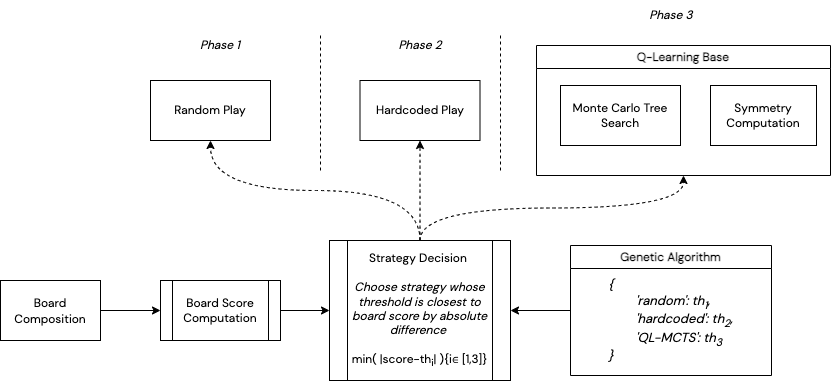
\includegraphics[width=0.9\textwidth]{images/methodology.drawio.png}
    \caption{Hybrid Agent}
    \label{fig:hybrid-agent}
\end{figure}

The main question is when to switch between the algorithms. The intuition is that the switch depends on the change of the board composition. We represent this numerically through a board score, that is essentially a sum of couplets and triplets.

\begin{equation*}
    couples + 2 * triplets
\end{equation*}

The range of values for scores $\in [0, 16]$. We try to generate score thresholds to switch between the 3 strategies using a genetic algorithm. An example of a genome is shown in Figure \ref{json-example}.

\begin{listing}
    \begin{minted}{json}
    {
        "random": 3,
        "hardcoded" : 5,
        "ql-mcts" : 8
    }
    \end{minted}
    \caption{Genome Example}
    \label{json-example}
    \end{listing}

We train the genetic algorithm for 1000 generations and a population size of 100, to find the best genome and submit these as the thresholds for the hybrid agent.

Once the final thresholds are found, we find the strategy whose threshold has the smallest absolute difference with the current board score. The minimisation formula is:

\begin{equation*}
    \text{strategy} = \min_{i=1}^{3} \left| \text{threshold}_i - \text{board score} \right|
\end{equation*}

\subsection{Results}

After several iterations of the genetic algorithm, the best genome thresholds were found to be:

\begin{minted}{json}
{
    'random': 2.090773081612301,
    'hardcoded': 3.790328881747581,
    'ql-mcts': 7.251997327518943
}
\end{minted}

It is clear that the algorithm prefers to use the QL-MCTS (essentially MCTS) strategy extensively, as it almost always guarantees a win regardless of whether it is playing first or second. Random is entirely probabilistic and hardcoded has better chances only when it's the first player.

Tournament results are shown in Table \ref{results}, where each player is played against a random player for 10 tournaments of 10 games each (10 x 10 = 100 games).

% put in table
\begin{table}[h]
    \centering
    \begin{tabular}{|c|c|c|}
        \hline
        \textbf{Strategy} & \textbf{Win Rate} & \textbf{Comments} \\ \hline
        DQN & 55\% & Convergence not reached \\ \hline
        QL-MCTS & 84\% & Slow, but can guarantee a win \\ \hline
        Hardcoded & 94\% & Fast \\ \hline
        Hybrid & 78\% & Heavily dependent on adjusting thresholds \\ \hline
    \end{tabular}
    \caption{Results computed based on 10 tournaments of 10 games each (10 x 10 = 100 games) against a random player}
    \label{results}
\end{table}

\subsection{Code of Hybrid Agent and Sub Players}

This subsection covers the code of the final hybrid agent and the sub players it calls periodically.

\subsubsection{Final Hybrid Player}

The final hybrid player's driver code is below. It uses a genetic algorithm to find the best thresholds for switching between the 3 strategies. It uses crossover and conditional mutations to find the best genome from a limited population size.

Furthermore, to reduce the search space, we enforce the constraint that the threshold for random < hardcoded < MCTS, with the the intuition that the slowest but most powerful algorithm should be used last.

\begin{mintedbox}{python}
'''
Genetic Algorithm for Quarto
'''
import os
import sys
sys.path.insert(0, '..')

import tqdm
import random
import logging
import json
import itertools
from copy import deepcopy
from lib.players import Player, RandomPlayer
from quarto.objects import Quarto
from lib.scoring import score_board
from QLMCTS import QLearningPlayer
from Hardcoded.hardcoded import HardcodedPlayer

logging.basicConfig(level=logging.DEBUG)

class Genome:
    def __init__(self, thresholds, fitness):
        self.thresholds = thresholds
        self.fitness = fitness

    def set_fitness(self, fitness):
        self.fitness = fitness

    def set_thresholds(self, thresholds):
        self.thresholds = thresholds

    def toJSON(self):
        return {
            'thresholds': self.thresholds,
            'fitness': self.fitness
        }


class FinalPlayer(Player):
    '''
    Final player uses genetic algorithm to decide between:
    1. Hardcoded Strategy
    2. Random Strategy
    3. QL-MCTS
    '''

    def __init__(self, quarto: Quarto = None):
        if quarto is None:
            quarto = Quarto()
        super().__init__(quarto)
        self.ql_mcts = QLearningPlayer(quarto)
        self.hardcoded = HardcodedPlayer(quarto)
        self.random_player = RandomPlayer(quarto)
        self.BOARD_SIDE = 4
        self.GENOME_VAL_UPPER_BOUND = 16
        self.GENOME_VAL_LOWER_BOUND = 0
        self.thresholds = {
            'random': 1.090773081612301,
            'hardcoded': 2.790328881747581,
            'ql-mcts': 6.251997327518943
        }
        self.ql_mcts_next_piece = -1

    def generate_population(self, population_size):
        population = []
        for i in range(population_size):
            threshold = {}

            # make sure that value for random < hardcoded < ql-mcts
            threshold['random'] = random.random() * self.GENOME_VAL_UPPER_BOUND
            # find random number between random and 15
            threshold['hardcoded'] = threshold['random'] + \
                random.random() * (self.GENOME_VAL_UPPER_BOUND -
                                    threshold['random'])

            # find random number between hardcoded and 15
            threshold['ql-mcts'] = threshold['hardcoded'] + \
                random.random() * (self.GENOME_VAL_UPPER_BOUND -
                                    threshold['hardcoded'])

            assert threshold['random'] < threshold['hardcoded'] < threshold['ql-mcts']

            population.append(Genome(threshold, 0))
        return population

    def ensure_correct_ordering(self, new_thresholds):
        if new_thresholds['random'] > new_thresholds['hardcoded']:
            new_thresholds['random'], new_thresholds['hardcoded'] = new_thresholds['hardcoded'], new_thresholds['random']
        if new_thresholds['hardcoded'] > new_thresholds['ql-mcts']:
            new_thresholds['hardcoded'], new_thresholds['ql-mcts'] = new_thresholds['ql-mcts'], new_thresholds['hardcoded']
        if new_thresholds['random'] > new_thresholds['hardcoded']:
            new_thresholds['random'], new_thresholds['hardcoded'] = new_thresholds['hardcoded'], new_thresholds['random']
        return new_thresholds

    def crossover(self, genome1, genome2):
        new_thresholds = {}
        for key in genome1.thresholds:
            new_thresholds[key] = random.choice(
                [genome1.thresholds[key], genome2.thresholds[key]])

        # make sure that value for random < hardcoded < ql-mcts
        new_thresholds = self.ensure_correct_ordering(new_thresholds)
        return Genome(new_thresholds, 0)

    def mutate(self, genome):
        new_thresholds = {}
        genome_thresholds = genome.thresholds
        if random.random() < 0.4:
            new_thresholds['random'] = random.random() * \
                self.GENOME_VAL_UPPER_BOUND
            new_thresholds['hardcoded'] = random.choice(
                [genome_thresholds['random'], genome_thresholds['random'] +
                    random.random() * (self.GENOME_VAL_UPPER_BOUND - genome_thresholds['random'])])
            new_thresholds['ql-mcts'] = random.choice(
                [genome_thresholds['hardcoded'], genome_thresholds['hardcoded'] +
                    random.random() * (self.GENOME_VAL_UPPER_BOUND - genome_thresholds['hardcoded'])])

            new_thresholds = self.ensure_correct_ordering(new_thresholds)

            assert new_thresholds['random'] < new_thresholds['hardcoded'] < new_thresholds['ql-mcts']

            return Genome(new_thresholds, 0)
        return genome

    def evolve(self, num_generations=50):
        self.population_size = 50
        self.offspring_size = 10
        population = self.generate_population(self.population_size)

        pbar = tqdm.tqdm(total=num_generations)
        for gen in range(num_generations):
            pbar.update(1)
            logging.debug('Generation: {}'.format(gen))
            offpsring = []
            for i in range(self.offspring_size):
                parent1 = random.choice(population)
                parent2 = random.choice(population)
                child = self.crossover(parent1, parent2)
                child = self.mutate(child)
                child.fitness = self.play_game(child.thresholds, num_games=5)
                offpsring.append(child)
            population += offpsring
            population = sorted(
                population, key=lambda x: x.fitness, reverse=True)[:self.population_size]

            if gen % 5 == 0:
                logging.info('Saving population')
                with open('/Volumes/USB/population3.json', 'w') as f:
                    json.dump([genome.toJSON() for genome in population], f)

        # return the best genome's thresholds
        return population[0].thresholds

    def play_game(self, thresholds, num_games=10):
        wins = 0
        for game in range(num_games):
            logging.debug('Game: {}'.format(game))
            state = Quarto()
            player = 0

            # initialise with some random piece just to kickstart game
            state.set_selected_piece(self.random_player.choose_piece(state, 0))
            self.current_state = state

            # python passes by reference
            # agent will use the state, etc. to update the Q-table
            # this function also wipes the MCTS tree
            self.ql_mcts.clear_and_set_current_state(state)
            self.hardcoded = HardcodedPlayer(state)

            while True:
                # board score is the number of couples and triplets on the board
                # it is indicative of the change of the board state
                board_score = score_board(self.current_state)

                differences = [abs(board_score - thresholds[key])
                                for key in thresholds]
                min_diff = min(differences)
                index = differences.index(min_diff)
                key = list(thresholds.keys())[index]

                if player == 0:
                    if key == 'random':
                        logging.debug('random')
                        # play randomly
                        action = self.random_player.place_piece()
                        next_piece = self.random_player.choose_piece()
                        while self.current_state.check_if_move_valid(self.current_state.get_selected_piece(), action[0], action[1], next_piece) is False:
                            action = self.random_player.place_piece()
                            next_piece = self.random_player.choose_piece()
                        self.current_state.select(
                            self.current_state.get_selected_piece())
                        self.current_state.place(action[0], action[1])
                        self.current_state.set_selected_piece(next_piece)
                        self.current_state.switch_player()
                        player = 1 - player

                    elif key == 'hardcoded':
                        # play using hardcoded strategy
                        self.previous_state = deepcopy(self.current_state)
                        winning_piece, position = self.hardcoded.hardcoded_strategy_get_move()
                        next_piece = self.hardcoded.hardcoded_strategy_get_piece()
                        while self.current_state.check_if_move_valid(self.current_state.get_selected_piece(), position[0], position[1], next_piece) is False:
                            winning_piece, position = self.hardcoded.hardcoded_strategy_get_move()
                            next_piece = self.hardcoded.hardcoded_strategy_get_piece()
                        self.current_state.select(state.get_selected_piece())
                        self.current_state.place(position[0], position[1])
                        self.current_state.set_selected_piece(next_piece)
                        self.current_state.switch_player()
                        player = 1 - player

                    else:
                        # play using QL-MCTS
                        print('ql-mcts')
                        self.ql_mcts.previous_state = deepcopy(
                            self.current_state)
                        action = self.ql_mcts.get_action(self.current_state)
                        self.ql_mcts.previous_action = action
                        # store the next piece for when choose is called
                        # self.ql_mcts_next_piece = self.ql_mcts.tree.choose_piece()
                        self.ql_mcts_next_piece = self.ql_mcts.tree.choose_piece()
                        self.ql_mcts.current_state.select(
                            self.current_state.get_selected_piece())
                        self.ql_mcts.current_state.place(action[0], action[1])
                        self.ql_mcts.current_state.set_selected_piece(
                            self.ql_mcts_next_piece)
                        self.ql_mcts.current_state.switch_player()
                        player = 1 - player

                else:
                    # opponent is random
                    action = self.random_player.place_piece()
                    next_piece = self.random_player.choose_piece()
                    while self.current_state.check_if_move_valid(self.current_state.get_selected_piece(), action[0], action[1], next_piece) is False:
                        action = self.random_player.place_piece()
                        next_piece = self.random_player.choose_piece()
                        # WARNING: very often stuck in this loop
                    self.current_state.select(
                        self.current_state.get_selected_piece())
                    self.current_state.place(action[0], action[1])
                    self.current_state.set_selected_piece(next_piece)
                    self.current_state.switch_player()
                    player = 1 - player

                if self.current_state.check_is_game_over():
                    if 1 - self.current_state.check_winner() == 0:
                        print("Agent wins")
                        wins += 1
                        # TODO: QL reward update
                    else:
                        print("Player 2 wins")
                    break

        # fitness is the percentage of games won
        logging.debug(f"Win rate: {wins/num_games}")
        return wins/num_games

    def choose_piece(self):
        '''
        Choose piece for next player to place
        '''
        thresholds = self.thresholds

        # game is stored in parent
        self.current_state = self.get_game()

        board_score = score_board(self.current_state)

        differences = [abs(board_score - thresholds[key])
                        for key in thresholds]
        min_diff = min(differences)
        index = differences.index(min_diff)
        key = list(thresholds.keys())[index]

        # python passes by reference
        # agent will use the state, etc. to update the Q-table
        # this function also wipes the MCTS tree
        # self.ql_mcts.clear_and_set_current_state(self.current_state)
        self.hardcoded = HardcodedPlayer(self.current_state)

        if self.ql_mcts_next_piece != -1:
            if self.ql_mcts_next_piece not in list(itertools.chain(*self.current_state.state_as_array())):
                print('ql-mcts choose')
                return self.ql_mcts_next_piece

        if key == 'random':
            # play randomly
            next_piece = self.random_player.choose_piece()
            while next_piece in list(itertools.chain(*self.current_state.state_as_array())):
                next_piece = self.random_player.choose_piece()
            self.ql_mcts_next_piece = -1
            return next_piece

        # elif key == 'hardcoded':
        else:
            # play using hardcoded strategy
            print('hardcoded')
            self.previous_state = deepcopy(self.current_state)
            next_piece = self.hardcoded.hardcoded_strategy_get_piece()
            self.ql_mcts_next_piece = -1
            return next_piece

    def place_piece(self):
        # python passes by reference
        # agent will use the state, etc. to update the Q-table
        # this function also wipes the MCTS tree
        self.current_state = self.get_game()
        thresholds = self.thresholds

        # python passes by reference
        # agent will use the state, etc. to update the Q-table
        # this function also wipes the MCTS tree
        # self.ql_mcts.clear_and_set_current_state(self.current_state)

        self.hardcoded = HardcodedPlayer(self.current_state)

        while True:
            # board score is the number of couples and triplets on the board
            # it is indicative of the change of the board state
            board_score = score_board(self.current_state)

            differences = [abs(board_score - thresholds[key])
                            for key in thresholds]
            min_diff = min(differences)
            index = differences.index(min_diff)
            key = list(thresholds.keys())[index]

            if key == 'random':
                logging.debug('random')
                # play randomly
                action = self.random_player.place_piece()
                next_piece = self.random_player.choose_piece()
                while self.current_state.check_if_move_valid(self.current_state.get_selected_piece(), action[0], action[1], next_piece) is False:
                    action = self.random_player.place_piece()
                    next_piece = self.random_player.choose_piece()
                return action[0], action[1]

            elif key == 'hardcoded':
                # play using hardcoded strategy
                logging.debug('hardcoded')
                self.previous_state = deepcopy(self.current_state)
                winning_piece, position = self.hardcoded.hardcoded_strategy_get_move()
                # next_piece = self.hardcoded_strategy_get_piece()
                # while self.current_state.check_if_move_valid(self.current_state.get_selected_piece(), position[0], position[1], next_piece) is False:
                #     winning_piece, position = self.hardcoded_strategy_get_move()
                #     next_piece = self.hardcoded_strategy_get_piece()
                return position[0], position[1]

            else:
                # play using QL-MCTS
                logging.debug('ql-mcts')
                print(f"Selected piece: {self.current_state.get_selected_piece()}")
                self.ql_mcts.previous_state = deepcopy(
                    self.current_state)
                action = self.ql_mcts.get_action(self.current_state)
                self.ql_mcts.previous_action = action
                # store the next piece for when choose is called
                # self.ql_mcts_next_piece = self.ql_mcts.tree.choose_piece()
                self.ql_mcts_next_piece = self.ql_mcts.tree.choose_piece()
                return action[0], action[1]

    def test_thresholds(self):
        win_rate = self.play_game(self.thresholds, num_games=5)
        print(f"Win rate: {win_rate}")
        return win_rate

if __name__ == "__main__":
    final_player = FinalPlayer()
    average_win_rate = 0
    for i in range(10):
        win_rate = final_player.test_thresholds()
        average_win_rate += win_rate
    print(f"Average win rate: {average_win_rate}")
\end{mintedbox}

\subsubsection{Hardcoded Strategy}

The strategy is outlined in this \href{https://scholarworks.umt.edu/cgi/viewcontent.cgi?article=1334&context=tme}{paper}. I implement it in Python below.

\begin{mintedbox}{python}
'''
Hardcoded player for Quarto
Follows risky strategy from paper:

"Developing Strategic and Mathematical Thinking via Game Play:
Programming to Investigate a Risky Strategy for Quarto"
by Peter Rowlett
'''
from copy import deepcopy
import itertools
import logging
import random

from lib.players import Player
from quarto.objects import Quarto

import sys
sys.path.insert(0, '..')

class HardcodedPlayer(Player):
    def __init__(self, quarto: Quarto = None):
        if quarto is None:
            quarto = Quarto()
        super().__init__(quarto)
        self.BOARD_SIDE = 4

    def check_if_winning_piece(self, state, piece):
        '''
        Simulate placing the piece on the board and check if the game is over
        '''

        for i in range(self.BOARD_SIDE):
            for j in range(self.BOARD_SIDE):
                if state.check_if_move_valid(piece, i, j, -100):
                    cloned_state = deepcopy(state)
                    cloned_state.select(piece)
                    cloned_state.place(i, j)

                    if cloned_state.check_is_game_over():
                        return True, [i, j]
        return False, None

    def hardcoded_strategy_get_piece(self):
        '''
        Returns a piece to be placed on the board
        '''
        state = self.get_game()

        possible_pieces = []
        for i in range(16):
            # check if the piece is a winning piece
            winning_piece, _ = self.check_if_winning_piece(state, i)
            if (not winning_piece) and (i not in list(itertools.chain.from_iterable(state.state_as_array()))) and (i != state.get_selected_piece()):
                possible_pieces.append(i)

        # if no pieces can be placed on board anymore (board full/game over), return -1
        if len(possible_pieces) == 0:
            # check if number of non-empty cells is 16
            if len([i for i in list(itertools.chain.from_iterable(state.state_as_array())) if i != -1]) == 16:
                return -1
            else:
                # there are possible pieces to be placed, but they are winning pieces/already in board
                on_board = list(itertools.chain.from_iterable(
                    state.state_as_array()))
                not_on_board = list(set(range(16)) - set(on_board))
                return random.choice(not_on_board)
        else:
            return random.choice(possible_pieces)

    def choose_piece(self):
        '''
        Returns a piece to be placed on the board
        '''
        return self.hardcoded_strategy_get_piece()

    def hardcoded_strategy_get_move(self, return_winning_piece_boolean=True):
        #  1. Play the piece handed over by the opponent:
        # (a) play a winning position if handed a winning piece;
        # (b) otherwise, play to build a line of like pieces if possible;
        # (c) otherwise, play randomly.
        # 2. Hand a piece to the opponent:
        # (a) avoid handing over a winning piece for your opponent to play;
        # (b) otherwise, choose randomly.

        state = self.get_game()

        board = state.state_as_array()
        selected_piece = state.get_selected_piece()
        # check if the selected piece is a winning piece
        winning_piece, position = self.check_if_winning_piece(
            state, selected_piece)
        if winning_piece:
            return selected_piece, position

        # check if the selected piece can be used to build a line of like pieces

        row_1 = [[0, 0], [0, 1], [0, 2], [0, 3]]
        # pieces in row 2
        row_2 = [[1, 0], [1, 1], [1, 2], [1, 3]]
        # pieces in row 3
        row_3 = [[2, 0], [2, 1], [2, 2], [2, 3]]
        # pieces in row 4
        row_4 = [[3, 0], [3, 1], [3, 2], [3, 3]]

        # pieces in column 1
        col_1 = [[0, 0], [1, 0], [2, 0], [3, 0]]
        # pieces in column 2
        col_2 = [[0, 1], [1, 1], [2, 1], [3, 1]]
        # pieces in column 3
        col_3 = [[0, 2], [1, 2], [2, 2], [3, 2]]
        # pieces in column 4
        col_4 = [[0, 3], [1, 3], [2, 3], [3, 3]]

        # pieces in diagonal 1
        diag_1 = [[0, 0], [1, 1], [2, 2], [3, 3]]
        # pieces in diagonal 2
        diag_2 = [[0, 3], [1, 2], [2, 1], [3, 0]]

        for line in [row_1, row_2, row_3, row_4, col_1, col_2, col_3, col_4, diag_1, diag_2]:
            # check if the selected piece can be used to build a line of like pieces
            characteristics = []
            empty_rows = []
            for el in line:
                x, y = el
                if board[x, y] != -1:
                    piece = board[x][y]
                    piece_char = state.get_piece_charachteristics(piece)
                    characteristics.append(
                        [piece_char.HIGH, piece_char.COLOURED, piece_char.SOLID, piece_char.SQUARE])
                else:
                    empty_rows.append(el)
                    characteristics.append([-1, -1, -1, -1])

            selected_piece_char = state.get_piece_charachteristics(
                selected_piece)
            selected_piece_char = [selected_piece_char.HIGH, selected_piece_char.COLOURED,
                                    selected_piece_char.SOLID, selected_piece_char.SQUARE]

            # check if characteristics has an empty row
            if [-1, -1, -1, -1] in characteristics:
                # count how many [-1, -1, -1, -1] are in characteristics
                empty_indexes = [i for i, x in enumerate(
                    characteristics) if x == [-1, -1, -1, -1]]

                empty_rows_count = characteristics.count([-1, -1, -1, -1])
                characteristics_copy = characteristics.copy()

                # proceeding to check couplets and see if they can build triplets
                # since 2 empty rows may be present and either could create a triplet, have to choose randomly later
                potential_moves = []

                for i, index in enumerate(empty_indexes):
                    position = empty_rows[i]
                    # insert the selected piece in the empty row
                    # empty_piece_index = characteristics.index(
                    #     [-1, -1, -1, -1])
                    characteristics = characteristics_copy.copy()
                    characteristics[index] = selected_piece_char

                    # check if any column has the same characteristics
                    col1 = [characteristics[0][0], characteristics[1][0],
                            characteristics[2][0], characteristics[3][0]]
                    col2 = [characteristics[0][1], characteristics[1][1],
                            characteristics[2][1], characteristics[3][1]]
                    col3 = [characteristics[0][2], characteristics[1][2],
                            characteristics[2][2], characteristics[3][2]]
                    col4 = [characteristics[0][3], characteristics[1][3],
                            characteristics[2][3], characteristics[3][3]]

                    col1 = [int(i) for i in col1]
                    col2 = [int(i) for i in col2]
                    col3 = [int(i) for i in col3]
                    col4 = [int(i) for i in col4]

                    # print(col1, col2, col3, col4)
                    def check_if_form_triplet(line):
                        # earlier we checked if we can complete a line
                        # here we check if we can form a triplet (one step away from completing a line)
                        return line.count(1) == 3 or line.count(0) == 3

                    # if len(set(col1)) == 1 or len(set(col2)) == 1 or len(set(col3)) == 1 or len(set(col4)) == 1:
                    if check_if_form_triplet(col1) or check_if_form_triplet(col2) or check_if_form_triplet(col3) or check_if_form_triplet(col4):
                        # this piece can be used to build a line of like pieces
                        logging.debug('playing to build a line of like pieces')
                        potential_moves.append(list(reversed(position)))

                    if len(potential_moves) >= 1:
                        if return_winning_piece_boolean:
                            # return True, list(reversed(empty_rows[-1]))
                            return True, random.choice(potential_moves)
                        else:
                            # move = list(reversed(empty_rows[-1]))
                            # move = list(reversed(position))
                            move = random.choice(potential_moves)
                            return move[0], move[1]

        # play randomly
        possible_moves = []
        for i in range(self.BOARD_SIDE):
            for j in range(self.BOARD_SIDE):
                for next_piece in range(16):
                    if state.check_if_move_valid(selected_piece, i, j, next_piece):
                        if return_winning_piece_boolean:
                            possible_moves.append([False, [i, j]])
                        else:
                            possible_moves.append([i, j])

        random_move = random.choice(possible_moves)
        return random_move[0], random_move[1]

        logging.debug(f"Selected piece: {selected_piece}")
        logging.debug(f"Board: {board}")
        logging.debug('no move found')

    def place_piece(self):
        '''
        Above function sometimes necessary to return additional information
        In game, first return value is not necessary
        '''
        return self.hardcoded_strategy_get_move(return_winning_piece_boolean=False)
\end{mintedbox}

\subsubsection{Q-Learning + MCTS}

Here, I combine plain Q-Learning with an MCTS fallback, calling MCTS in the exploration hase and resorting to it in testing when a "state + action" pair cannot be found in the table.

\begin{mintedbox}{python}
from collections import defaultdict
from copy import deepcopy
import itertools
import json
import logging
import math
import os
import random
import time

from MCTS import MonteCarloTreeSearch
from MCTS.mcts import decode_tree
from quarto.objects import Quarto
from lib.players import Player, RandomPlayer
from lib.isomorphic import BoardTransforms

import tqdm
logging.basicConfig(level=logging.DEBUG)


class QLearningPlayer(Player):
    def __init__(self, board: Quarto = Quarto(), epsilon=0.1, alpha=0.5, gamma=0.9, tree: MonteCarloTreeSearch = None):
        self.epsilon = epsilon
        self.alpha = alpha
        self.gamma = gamma
        self.board = board
        self.MAX_PIECES = 16
        self.BOARD_SIDE = 4
        self.Q = defaultdict(int)

        if tree is not None:
            # load the pre-initalised tree
            self.tree = tree
            self.tree.set_board(board)

        else:
            # load new tree
            self.tree = MonteCarloTreeSearch(board=board)

        super().__init__(board)

    def clear_and_set_current_state(self, state: Quarto):
        self.current_state = state
        self.tree = MonteCarloTreeSearch(board=state)

    def reduce_normal_form(self, state: Quarto):
        '''
        Reduce the Quarto board to normal form (i.e. the board is symmetric)
        '''
        # NOT IMPLEMENTED for now, just return the board
        return state

    def hash_state_action(self, state: Quarto, action):
        # reduce to normal form before saving to Q table
        return state.board_to_string() + '||' + str(state.get_selected_piece()) + '||' + str(action)

    def get_Q(self, state, action):
        # check possible transforms first (really really slow)
        for key, val in self.Q.items():
            if BoardTransforms.compare_boards(state.state_as_array(), state.string_to_board(key.split('||')[0])):
                return val

        if self.hash_state_action(state, action) not in self.Q:
            # used to determine if state exists in Q table
            # if None, then go to MCTS
            return None

        return self.Q[self.hash_state_action(state, action)]

    def get_Q_for_state(self, state):
        if self.hash_state_action(state, None) not in self.Q:
            return None
        return [i for i in self.Q if i.startswith(str(state))]

    def set_Q(self, state, action, value):
        self.Q[self.hash_state_action(state, action)] = value

    def get_possible_actions(self, state: Quarto):
        actions = []
        for i in range(self.BOARD_SIDE):
            for j in range(self.BOARD_SIDE):
                for piece in range(self.MAX_PIECES):
                    if state.check_if_move_valid(self.board.get_selected_piece(), i, j, piece):
                        actions.append((i, j, piece))

        return actions

    def get_max_Q(self, state):
        max_Q = -math.inf
        for action in self.get_possible_actions(state):
            if self.get_Q(state, action) is not None:
                Q_val = self.get_Q(state, action)
                max_Q = max(max_Q, self.get_Q(state, action))
        return max_Q

    def check_if_winning_piece(self, state, piece):
        for i in range(self.BOARD_SIDE):
            for j in range(self.BOARD_SIDE):
                if state.check_if_move_valid(piece, i, j, piece):
                    cloned_state = deepcopy(state)
                    cloned_state.select(piece)
                    cloned_state.place(i, j)

                    if cloned_state.check_is_game_over():
                        print('WINNING PIECE FOUND')
                        return True, [i, j]
        return False, None

    def hardcoded_strategy_get_move(self, state):
        #  1. Play the piece handed over by the opponent:
        # (a) play a winning position if handed a winning piece;
        # (b) otherwise, play to build a line of like pieces if possible;
        # (c) otherwise, play randomly.
        # 2. Hand a piece to the opponent:
        # (a) avoid handing over a winning piece for your opponent to play;
        # (b) otherwise, choose randomly.

        board = state.state_as_array()
        selected_piece = state.get_selected_piece()
        # check if the selected piece is a winning piece
        winning_piece, position = self.check_if_winning_piece(
            state, selected_piece)
        if winning_piece:
            return selected_piece, position

        # check if the selected piece can be used to build a line of like pieces

        row_1 = [[0, 0], [0, 1], [0, 2], [0, 3]]
        # pieces in row 2
        row_2 = [[1, 0], [1, 1], [1, 2], [1, 3]]
        # pieces in row 3
        row_3 = [[2, 0], [2, 1], [2, 2], [2, 3]]
        # pieces in row 4
        row_4 = [[3, 0], [3, 1], [3, 2], [3, 3]]

        # pieces in column 1
        col_1 = [[0, 0], [1, 0], [2, 0], [3, 0]]
        # pieces in column 2
        col_2 = [[0, 1], [1, 1], [2, 1], [3, 1]]
        # pieces in column 3
        col_3 = [[0, 2], [1, 2], [2, 2], [3, 2]]
        # pieces in column 4
        col_4 = [[0, 3], [1, 3], [2, 3], [3, 3]]

        # pieces in diagonal 1
        diag_1 = [[0, 0], [1, 1], [2, 2], [3, 3]]
        # pieces in diagonal 2
        diag_2 = [[0, 3], [1, 2], [2, 1], [3, 0]]

        for line in [row_1, row_2, row_3, row_4, col_1, col_2, col_3, col_4, diag_1, diag_2]:
            # check if the selected piece can be used to build a line of like pieces
            characteristics = []
            empty_rows = []
            for el in line:
                x, y = el
                if board[x, y] != -1:
                    piece = board[x][y]
                    piece_char = state.get_piece_charachteristics(piece)
                    characteristics.append(
                        [piece_char.HIGH, piece_char.COLOURED, piece_char.SOLID, piece_char.SQUARE])
                else:
                    empty_rows.append(el)
                    characteristics.append([-1, -1, -1, -1])

            selected_piece_char = state.get_piece_charachteristics(
                selected_piece)
            selected_piece_char = [selected_piece_char.HIGH, selected_piece_char.COLOURED,
                                    selected_piece_char.SOLID, selected_piece_char.SQUARE]

            # check if characteristics has an empty row
            if [-1, -1, -1, -1] in characteristics:
                # insert the selected piece in the empty row
                empty_piece_index = characteristics.index(
                    [-1, -1, -1, -1])
                characteristics[empty_piece_index] = selected_piece_char

                # check if any column has the same characteristics
                col1 = [characteristics[0][0], characteristics[1][0],
                        characteristics[2][0], characteristics[3][0]]
                col2 = [characteristics[0][1], characteristics[1][1],
                        characteristics[2][1], characteristics[3][1]]
                col3 = [characteristics[0][2], characteristics[1][2],
                        characteristics[2][2], characteristics[3][2]]
                col4 = [characteristics[0][3], characteristics[1][3],
                        characteristics[2][3], characteristics[3][3]]

                col1 = [int(i) for i in col1]
                col2 = [int(i) for i in col2]
                col3 = [int(i) for i in col3]
                col4 = [int(i) for i in col4]

                if len(set(col1)) == 1 or len(set(col2)) == 1 or len(set(col3)) == 1 or len(set(col4)) == 1:
                    # this piece can be used to build a line of like pieces
                    logging.debug('playing to build a line of like pieces')
                    return True, list(reversed(empty_rows[-1]))

        # play randomly
        for i in range(self.BOARD_SIDE):
            for j in range(self.BOARD_SIDE):
                for next_piece in range(16):
                    if state.check_if_move_valid(selected_piece, i, j, next_piece):
                        return False, [i, j]

        print('returning nothing')
        print(state.state_as_array())
        print(state.get_selected_piece())

    def hardcoded_strategy_get_piece(self, state):
        possible_pieces = []
        for i in range(16):
            # check if the piece is a winning piece
            winning_piece, _ = self.check_if_winning_piece(state, i)
            if (not winning_piece) and (i not in list(itertools.chain.from_iterable(state.state_as_array()))) and (i != state.get_selected_piece()):
                possible_pieces.append(i)

        return random.choice(possible_pieces)

    def get_action(self, state, mode='training'):
        '''
        If state, action pair not in Q, go to Monte Carlo Tree Search to find best action
        '''
        if mode == 'training':
            # exploration through epsilon greedy
            # look for good moves through Monte Carlo Tree Search
            if random.random() < self.epsilon:
                for i in range(20):
                    self.tree.do_rollout(state)
                best_action = self.tree.place_piece()
                return best_action
            else:
                # look in the q table for the best action
                expected_score = 0
                best_action = None
                for action in self.get_possible_actions(state):
                    if self.get_Q(state, action) is not None and expected_score < self.get_Q(state, action):
                        print('found in Q table')
                        expected_score = self.get_Q(state, action)
                        best_action = action
                # go to Monte Carlo Tree Search if no suitable action found in Q table
                if best_action is None or expected_score == 0:
                    logging.debug(
                        'No suitable action found in Q table, going to Monte Carlo Tree Search')
                    for i in range(20):
                        self.tree.do_rollout(state)
                    best_action = self.tree.place_piece()
                else:
                    print('found in Q table')

                return best_action
        else:
            # in test mode, use the Q table to find the best action
            # only go to Monte Carlo Tree Search if no suitable action found in Q table
            expected_score = 0
            best_action = None
            for action in self.get_possible_actions(state):
                if self.get_Q(state, action) is not None and expected_score < self.get_Q(state, action):
                    expected_score = self.get_Q(state, action)
                    best_action = action
            # go to Monte Carlo Tree Search if no suitable action found in Q table
            if best_action is None or expected_score == 0:
                logging.debug(
                    'No suitable action found in Q table, going to Monte Carlo Tree Search')
                for i in range(50):
                    self.tree.do_rollout(state)
                best_action = self.tree.place_piece()
            return best_action

    def update_Q(self, state, action, reward, next_state):
        Q_val = self.get_Q(state, action)
        if Q_val is None:
            Q_val = random.uniform(1.0, 0.01)
        self.set_Q(state, action, Q_val + self.alpha *
                    (reward + self.gamma * self.get_max_Q(next_state) - Q_val))

    def train(self, iterations=100):
        # 1. Use the Q-function to initialize the value of each state-action pair, Q(s, a) = 0.
        # automatically done through defaultdict

        # Choose an action using MCTS
        wins = 0
        tries = 0
        agent_decision_times = []

        progress_bar = tqdm.tqdm(total=iterations)
        for i in range(iterations):
            board = Quarto()
            self.board = board
            random_player = RandomPlayer(board)
            self.tree.set_board(board)
            self.current_state = board
            self.previous_state = None
            self.previous_action = None
            player = 1
            self.current_state.switch_player()
            selected_piece = random_player.choose_piece()
            self.current_state.set_selected_piece(selected_piece)
            while True:
                reward = 0
                if player == 0:
                    # QL-MCTS moves here
                    self.previous_state = deepcopy(self.current_state)
                    logging.debug("Piece to place: ",
                                    self.current_state.get_selected_piece())
                    logging.debug("Board: ")
                    logging.debug(self.current_state.state_as_array())
                    time_start = time.time()
                    action = self.get_action(self.current_state)
                    self.previous_action = action
                    time_end = time.time()
                    agent_decision_times.append(time_end - time_start)
                    self.current_state.select(selected_piece)
                    self.current_state.place(action[0], action[1])
                    self.current_state.set_selected_piece(action[2])
                    self.current_state.switch_player()
                    player = 1 - player

                else:
                    # Random moves here
                    action = random_player.place_piece()
                    next_piece = random_player.choose_piece()
                    while self.board.check_if_move_valid(self.board.get_selected_piece(), action[0], action[1], next_piece) is False:
                        action = random_player.place_piece()
                        next_piece = random_player.choose_piece()
                    self.current_state.select(
                        self.current_state.get_selected_piece())
                    self.current_state.place(action[0], action[1])
                    self.current_state.set_selected_piece(next_piece)
                    self.current_state.switch_player()
                    player = 1 - player

                if self.current_state.check_is_game_over():
                    if 1 - self.current_state.check_winner() == 1:
                        logging.info('QL-MCTS won')
                        reward = 1
                        wins += 1
                    else:
                        logging.info('Random won')
                        reward = -1
                    self.update_Q(self.previous_state, self.previous_action,
                                    reward, self.current_state)
                    break
                else:
                    if self.previous_state is not None:
                        self.update_Q(
                            self.previous_state, self.previous_action, reward, self.current_state)

            tries += 1
            if i % 10 == 0:
                logging.info(f'Iteration {i}')
                logging.info(f'Wins: {wins}')
                logging.info(f'Tries: {tries}')
                logging.info(f'Win rate: {wins/tries}')
                wins = 0
                tries = 0

            # OPTION 1: clear the tree every time
            self.tree = MonteCarloTreeSearch(board=self.board)

            # OPTION 2: if average agent decision time is too long, clear the MCTS tree
            # if sum(agent_decision_times) / len(agent_decision_times) > 5:
            #     self.tree = MonteCarloTreeSearch(board=self.board)
            #     agent_decision_times = []

            progress_bar.update(1)


if __name__ == '__main__':
    # load tree with MonteCarloSearchDecoder
    with open('progress.json', 'r') as f:
        tree = decode_tree(json.load(f))
    qplayer = QLearningPlayer()
    qplayer.train(10)

\end{mintedbox}

\subsection{Utility Functions}

\begin{mintedbox}{python}
def score_board(state: Quarto):
    positions = {
        'couples': 0,
        'triplets': 0,
    }

    board = state.state_as_array()

    # Array for checking if a certain row already contains a triplet
    row_done = [False, False, False, False]

    # Check all the rows

    for i in range(state.BOARD_SIDE):
        if board[i, 0] != -1 and board[i, 1] != -1 and board[i, 2] != -1 and board[i, 3] == -1:
            piece_1 = state.get_piece_charachteristics(board[i, 0])
            piece_2 = state.get_piece_charachteristics(board[i, 1])
            piece_3 = state.get_piece_charachteristics(board[i, 2])
            if piece_1.HIGH == piece_2.HIGH and piece_3.HIGH == piece_2.HIGH and piece_1.HIGH == True:
                positions['triplets'] += 1
                row_done[i] = True
            if piece_1.HIGH == piece_2.COLOURED and piece_3.COLOURED == piece_2.COLOURED and piece_1.COLOURED == True:
                positions['triplets'] += 1
                row_done[i] = True
            if piece_1.SQUARE == piece_2.SQUARE and piece_3.SQUARE == piece_2.SQUARE and piece_1.SQUARE == True:
                positions['triplets'] += 1
                row_done[i] = True
            if piece_1.SOLID == piece_2.SOLID and piece_3.SOLID == piece_2.SOLID and piece_1.SOLID == True:
                positions['triplets'] += 1
                row_done[i] = True
        if board[i, 0] == -1 and board[i, 1] != -1 and board[i, 2] != -1 and board[i, 3] != -1:
            piece_1 = state.get_piece_charachteristics(board[i, 1])
            piece_2 = state.get_piece_charachteristics(board[i, 2])
            piece_3 = state.get_piece_charachteristics(board[i, 3])
            if piece_1.HIGH == piece_2.HIGH and piece_3.HIGH == piece_2.HIGH and piece_1.HIGH == True:
                positions['triplets'] += 1
                row_done[i] = True
            if piece_1.COLOURED == piece_2.COLOURED and piece_3.COLOURED == piece_2.COLOURED and piece_1.COLOURED == True:
                positions['triplets'] += 1
                row_done[i] = True
            if piece_1.SQUARE == piece_2.SQUARE and piece_3.SQUARE == piece_2.SQUARE and piece_1.SQUARE == True:
                positions['triplets'] += 1
                row_done[i] = True
            if piece_1.SOLID == piece_2.SOLID and piece_3.SOLID == piece_2.SOLID and piece_1.SOLID == True:
                positions['triplets'] += 1
                row_done[i] = True
        if board[i, 0] != -1 and board[i, 1] != -1 and board[i, 2] == -1 and board[i, 3] != -1:
            piece_1 = state.get_piece_charachteristics(board[i, 0])
            piece_2 = state.get_piece_charachteristics(board[i, 1])
            piece_3 = state.get_piece_charachteristics(board[i, 3])
            if piece_1.HIGH == piece_2.HIGH and piece_3.HIGH == piece_2.HIGH and piece_1.HIGH == True:
                positions['triplets'] += 1
                row_done[i] = True
            if piece_1.COLOURED == piece_2.COLOURED and piece_3.COLOURED == piece_2.COLOURED and piece_1.COLOURED == True:
                positions['triplets'] += 1
                row_done[i] = True
            if piece_1.SQUARE == piece_2.SQUARE and piece_3.SQUARE == piece_2.SQUARE and piece_1.SQUARE == True:
                positions['triplets'] += 1
                row_done[i] = True
            if piece_1.SOLID == piece_2.SOLID and piece_3.SOLID == piece_2.SOLID and piece_1.SOLID == True:
                positions['triplets'] += 1
                row_done[i] = True
        if board[i, 0] != -1 and board[i, 1] == -1 and board[i, 2] != -1 and board[i, 3] != -1:
            piece_1 = state.get_piece_charachteristics(board[i, 0])
            piece_2 = state.get_piece_charachteristics(board[i, 2])
            piece_3 = state.get_piece_charachteristics(board[i, 3])
            if piece_1.HIGH == piece_2.HIGH and piece_3.HIGH == piece_2.HIGH and piece_1.HIGH == True:
                positions['triplets'] += 1
                row_done[i] = True
            if piece_1.COLOURED == piece_2.COLOURED and piece_3.COLOURED == piece_2.COLOURED and piece_1.COLOURED == True:
                positions['triplets'] += 1
                row_done[i] = True
            if piece_1.SQUARE == piece_2.SQUARE and piece_3.SQUARE == piece_2.SQUARE and piece_1.SQUARE == True:
                positions['triplets'] += 1
                row_done[i] = True
            if piece_1.SOLID == piece_2.SOLID and piece_3.SOLID == piece_2.SOLID and piece_1.SOLID == True:
                positions['triplets'] += 1
                row_done[i] = True
        # Before checking a row for couples, control the boolean flag
        if not row_done[i] and board[i, 0] != -1 and board[i, 1] != -1 and board[i, 2] == -1 and board[i, 3] == -1:
            piece_1 = state.get_piece_charachteristics(board[i, 0])
            piece_2 = state.get_piece_charachteristics(board[i, 1])
            if piece_1.HIGH == piece_2.HIGH and piece_1.HIGH == True:
                positions['couples'] += 1
            if piece_1.COLOURED == piece_2.COLOURED and piece_1.COLOURED == True:
                positions['couples'] += 1
            if piece_1.SQUARE == piece_2.SQUARE and piece_1.SQUARE == True:
                positions['couples'] += 1
            if piece_1.SOLID == piece_2.SOLID and piece_1.SOLID == True:
                positions['couples'] += 1
        if not row_done[i] and board[i, 0] == -1 and board[i, 1] != -1 and board[i, 2] != -1 and board[i, 3] == -1:
            piece_1 = state.get_piece_charachteristics(board[i, 1])
            piece_2 = state.get_piece_charachteristics(board[i, 2])
            if piece_1.HIGH == piece_2.HIGH and piece_1.HIGH == True:
                positions['couples'] += 1
            if piece_1.COLOURED == piece_2.COLOURED and piece_1.COLOURED == True:
                positions['couples'] += 1
            if piece_1.SQUARE == piece_2.SQUARE and piece_1.SQUARE == True:
                positions['couples'] += 1
            if piece_1.SOLID == piece_2.SOLID and piece_1.SOLID == True:
                positions['couples'] += 1
        if not row_done[i] and board[i, 0] == -1 and board[i, 1] == -1 and board[i, 2] != -1 and board[i, 3] != -1:
            piece_1 = state.get_piece_charachteristics(board[i, 2])
            piece_2 = state.get_piece_charachteristics(board[i, 3])
            if piece_1.HIGH == piece_2.HIGH and piece_1.HIGH == True:
                positions['couples'] += 1
            if piece_1.COLOURED == piece_2.COLOURED and piece_1.COLOURED == True:
                positions['couples'] += 1
            if piece_1.SQUARE == piece_2.SQUARE and piece_1.SQUARE == True:
                positions['couples'] += 1
            if piece_1.SOLID == piece_2.SOLID and piece_1.SOLID == True:
                positions['couples'] += 1

    # Array for checking if a certain column already contains a triplet
    column_done = [False, False, False, False]

    # Check all the columns

    for i in range(state.BOARD_SIDE):
        if board[0, i] != -1 and board[1, i] != -1 and board[2, i] != -1 and board[3, i] == -1:
            piece_1 = state.get_piece_charachteristics(board[0, i])
            piece_2 = state.get_piece_charachteristics(board[1, i])
            piece_3 = state.get_piece_charachteristics(board[2, i])
            if piece_1.HIGH == piece_2.HIGH and piece_3.HIGH == piece_2.HIGH and piece_1.HIGH == True:
                positions['triplets'] += 1
                column_done[i] = True
            if piece_1.HIGH == piece_2.COLOURED and piece_3.COLOURED == piece_2.COLOURED and piece_1.COLOURED == True:
                positions['triplets'] += 1
                column_done[i] = True
            if piece_1.SQUARE == piece_2.SQUARE and piece_3.SQUARE == piece_2.SQUARE and piece_1.SQUARE == True:
                positions['triplets'] += 1
                column_done[i] = True
            if piece_1.SOLID == piece_2.SOLID and piece_3.SOLID == piece_2.SOLID and piece_1.SOLID == True:
                positions['triplets'] += 1
                column_done[i] = True
        if board[0, i] == -1 and board[1, i] != -1 and board[2, i] != -1 and board[3, i] != -1:
            piece_1 = state.get_piece_charachteristics(board[1, i])
            piece_2 = state.get_piece_charachteristics(board[2, i])
            piece_3 = state.get_piece_charachteristics(board[3, i])
            if piece_1.HIGH == piece_2.HIGH and piece_3.HIGH == piece_2.HIGH and piece_1.HIGH == True:
                positions['triplets'] += 1
                column_done[i] = True
            if piece_1.COLOURED == piece_2.COLOURED and piece_3.COLOURED == piece_2.COLOURED and piece_1.COLOURED == True:
                positions['triplets'] += 1
                column_done[i] = True
            if piece_1.SQUARE == piece_2.SQUARE and piece_3.SQUARE == piece_2.SQUARE and piece_1.SQUARE == True:
                positions['triplets'] += 1
                column_done[i] = True
            if piece_1.SOLID == piece_2.SOLID and piece_3.SOLID == piece_2.SOLID and piece_1.SOLID == True:
                positions['triplets'] += 1
                column_done[i] = True
        if board[0, i] != -1 and board[1, i] == -1 and board[2, i] != -1 and board[3, i] != -1:
            piece_1 = state.get_piece_charachteristics(board[0, i])
            piece_2 = state.get_piece_charachteristics(board[2, i])
            piece_3 = state.get_piece_charachteristics(board[3, i])
            if piece_1.HIGH == piece_2.HIGH and piece_3.HIGH == piece_2.HIGH and piece_1.HIGH == True:
                positions['triplets'] += 1
                column_done[i] = True
            if piece_1.COLOURED == piece_2.COLOURED and piece_3.COLOURED == piece_2.COLOURED and piece_1.COLOURED == True:
                positions['triplets'] += 1
                column_done[i] = True
            if piece_1.SQUARE == piece_2.SQUARE and piece_3.SQUARE == piece_2.SQUARE and piece_1.SQUARE == True:
                positions['triplets'] += 1
                column_done[i] = True
            if piece_1.SOLID == piece_2.SOLID and piece_3.SOLID == piece_2.SOLID and piece_1.SOLID == True:
                positions['triplets'] += 1
                column_done[i] = True
        if board[0, i] != -1 and board[1, i] != -1 and board[2, i] == -1 and board[3, i] != -1:
            piece_1 = state.get_piece_charachteristics(board[0, i])
            piece_2 = state.get_piece_charachteristics(board[1, i])
            piece_3 = state.get_piece_charachteristics(board[3, i])
            if piece_1.HIGH == piece_2.HIGH and piece_3.HIGH == piece_2.HIGH and piece_1.HIGH == True:
                positions['triplets'] += 1
                column_done[i] = True
            if piece_1.COLOURED == piece_2.COLOURED and piece_3.COLOURED == piece_2.COLOURED and piece_1.COLOURED == True:
                positions['triplets'] += 1
                column_done[i] = True
            if piece_1.SQUARE == piece_2.SQUARE and piece_3.SQUARE == piece_2.SQUARE and piece_1.SQUARE == True:
                positions['triplets'] += 1
                column_done[i] = True
            if piece_1.SOLID == piece_2.SOLID and piece_3.SOLID == piece_2.SOLID and piece_1.SOLID == True:
                positions['triplets'] += 1
                column_done[i] = True
        # Before checking a column for couples, control the boolean flag
        if not column_done[i] and board[0, i] != -1 and board[1, i] != -1 and board[2, i] == -1 and board[3, i] == -1:
            piece_1 = state.get_piece_charachteristics(board[0, i])
            piece_2 = state.get_piece_charachteristics(board[1, i])
            if piece_1.HIGH == piece_2.HIGH and piece_1.HIGH == True:
                positions['couples'] += 1
            if piece_1.COLOURED == piece_2.COLOURED and piece_1.COLOURED == True:
                positions['couples'] += 1
            if piece_1.SQUARE == piece_2.SQUARE and piece_1.SQUARE == True:
                positions['couples'] += 1
            if piece_1.SOLID == piece_2.SOLID and piece_1.SOLID == True:
                positions['couples'] += 1
        if not column_done[i] and board[0, i] == -1 and board[1, i] != -1 and board[2, i] != -1 and board[3, i] == -1:
            piece_1 = state.get_piece_charachteristics(board[1, i])
            piece_2 = state.get_piece_charachteristics(board[2, i])
            if piece_1.HIGH == piece_2.HIGH and piece_1.HIGH == True:
                positions['couples'] += 1
            if piece_1.COLOURED == piece_2.COLOURED and piece_1.COLOURED == True:
                positions['couples'] += 1
            if piece_1.SQUARE == piece_2.SQUARE and piece_1.SQUARE == True:
                positions['couples'] += 1
            if piece_1.SOLID == piece_2.SOLID and piece_1.SOLID == True:
                positions['couples'] += 1
        if not column_done[i] and board[0, i] == -1 and board[1, i] == -1 and board[2, i] != -1 and board[3, i] != -1:
            piece_1 = state.get_piece_charachteristics(board[2, i])
            piece_2 = state.get_piece_charachteristics(board[3, i])
            if piece_1.HIGH == piece_2.HIGH and piece_1.HIGH == True:
                positions['couples'] += 1
            if piece_1.COLOURED == piece_2.COLOURED and piece_1.COLOURED == True:
                positions['couples'] += 1
            if piece_1.SQUARE == piece_2.SQUARE and piece_1.SQUARE == True:
                positions['couples'] += 1
            if piece_1.SOLID == piece_2.SOLID and piece_1.SOLID == True:
                positions['couples'] += 1

    # Array for checking if a certain diagonal already contains a triplet
    diagonal_done = [False, False]

    # Check first diagonal

    if board[0, 0] != -1 and board[1, 1] != -1 and board[2, 2] != -1 and board[3, 3] == -1:
        piece_1 = state.get_piece_charachteristics(board[0, 0])
        piece_2 = state.get_piece_charachteristics(board[1, 1])
        piece_3 = state.get_piece_charachteristics(board[2, 2])
        if piece_1.HIGH == piece_2.HIGH and piece_3.HIGH == piece_2.HIGH and piece_1.HIGH == True:
            positions['triplets'] += 1
            diagonal_done[0] = True
        if piece_1.COLOURED == piece_2.COLOURED and piece_3.COLOURED == piece_2.COLOURED and piece_1.COLOURED == True:
            positions['triplets'] += 1
            diagonal_done[0] = True
        if piece_1.SQUARE == piece_2.SQUARE and piece_3.SQUARE == piece_2.SQUARE and piece_1.SQUARE == True:
            positions['triplets'] += 1
            diagonal_done[0] = True
        if piece_1.SOLID == piece_2.SOLID and piece_3.SOLID == piece_2.SOLID and piece_1.SOLID == True:
            positions['triplets'] += 1
            diagonal_done[0] = True
    if board[0, 0] == -1 and board[1, 1] != -1 and board[2, 2] != -1 and board[3, 3] != -1:
        piece_1 = state.get_piece_charachteristics(board[1, 1])
        piece_2 = state.get_piece_charachteristics(board[2, 2])
        piece_3 = state.get_piece_charachteristics(board[3, 3])
        if piece_1.HIGH == piece_2.HIGH and piece_3.HIGH == piece_2.HIGH and piece_1.HIGH == True:
            positions['triplets'] += 1
            diagonal_done[0] = True
        if piece_1.COLOURED == piece_2.COLOURED and piece_3.COLOURED == piece_2.COLOURED and piece_1.COLOURED == True:
            positions['triplets'] += 1
            diagonal_done[0] = True
        if piece_1.SQUARE == piece_2.SQUARE and piece_3.SQUARE == piece_2.SQUARE and piece_1.SQUARE == True:
            positions['triplets'] += 1
            diagonal_done[0] = True
        if piece_1.SOLID == piece_2.SOLID and piece_3.SOLID == piece_2.SOLID and piece_1.SOLID == True:
            positions['triplets'] += 1
            diagonal_done[0] = True
    if board[0, 0] != -1 and board[1, 1] == -1 and board[2, 2] != -1 and board[3, 3] != -1:
        piece_1 = state.get_piece_charachteristics(board[0, 0])
        piece_2 = state.get_piece_charachteristics(board[2, 2])
        piece_3 = state.get_piece_charachteristics(board[3, 3])
        if piece_1.HIGH == piece_2.HIGH and piece_3.HIGH == piece_2.HIGH and piece_1.HIGH == True:
            positions['triplets'] += 1
            diagonal_done[0] = True
        if piece_1.COLOURED == piece_2.COLOURED and piece_3.COLOURED == piece_2.COLOURED and piece_1.COLOURED == True:
            positions['triplets'] += 1
            diagonal_done[0] = True
        if piece_1.SQUARE == piece_2.SQUARE and piece_3.SQUARE == piece_2.SQUARE and piece_1.SQUARE == True:
            positions['triplets'] += 1
            diagonal_done[0] = True
        if piece_1.SOLID == piece_2.SOLID and piece_3.SOLID == piece_2.SOLID and piece_1.SOLID == True:
            positions['triplets'] += 1
            diagonal_done[0] = True
    if board[0, 0] != -1 and board[1, 1] != -1 and board[2, 2] == -1 and board[3, 3] != -1:
        piece_1 = state.get_piece_charachteristics(board[0, 0])
        piece_2 = state.get_piece_charachteristics(board[1, 1])
        piece_3 = state.get_piece_charachteristics(board[3, 3])
        if piece_1.HIGH == piece_2.HIGH and piece_3.HIGH == piece_2.HIGH and piece_1.HIGH == True:
            positions['triplets'] += 1
            diagonal_done[0] = True
        if piece_1.COLOURED == piece_2.COLOURED and piece_3.COLOURED == piece_2.COLOURED and piece_1.COLOURED == True:
            positions['triplets'] += 1
            diagonal_done[0] = True
        if piece_1.SQUARE == piece_2.SQUARE and piece_3.SQUARE == piece_2.SQUARE and piece_1.SQUARE == True:
            positions['triplets'] += 1
            diagonal_done[0] = True
        if piece_1.SOLID == piece_2.SOLID and piece_3.SOLID == piece_2.SOLID and piece_1.SOLID == True:
            positions['triplets'] += 1
            diagonal_done[0] = True
    # Before checking a diagonal for couples, control the boolean flag
    if not diagonal_done[0] and board[0, 0] != -1 and board[1, 1] != -1 and board[2, 2] == -1 and board[3, 3] == -1:
        piece_1 = state.get_piece_charachteristics(board[0, 0])
        piece_2 = state.get_piece_charachteristics(board[1, 1])
        if piece_1.HIGH == piece_2.HIGH and piece_1.HIGH == True:
            positions['couples'] += 1
        if piece_1.COLOURED == piece_2.COLOURED and piece_1.COLOURED == True:
            positions['couples'] += 1
        if piece_1.SQUARE == piece_2.SQUARE and piece_1.SQUARE == True:
            positions['couples'] += 1
        if piece_1.SOLID == piece_2.SOLID and piece_1.SOLID == True:
            positions['couples'] += 1
    if not diagonal_done[0] and board[0, 0] == -1 and board[1, 1] != -1 and board[2, 2] != -1 and board[3, 3] == -1:
        piece_1 = state.get_piece_charachteristics(board[1, 1])
        piece_2 = state.get_piece_charachteristics(board[2, 2])
        if piece_1.HIGH == piece_2.HIGH and piece_1.HIGH == True:
            positions['couples'] += 1
        if piece_1.COLOURED == piece_2.COLOURED and piece_1.COLOURED == True:
            positions['couples'] += 1
        if piece_1.SQUARE == piece_2.SQUARE and piece_1.SQUARE == True:
            positions['couples'] += 1
        if piece_1.SOLID == piece_2.SOLID and piece_1.SOLID == True:
            positions['couples'] += 1
    if not diagonal_done[0] and board[0, 0] == -1 and board[1, 1] == -1 and board[2, 2] != -1 and board[3, 3] != -1:
        piece_1 = state.get_piece_charachteristics(board[2, 2])
        piece_2 = state.get_piece_charachteristics(board[3, 3])
        if piece_1.HIGH == piece_2.HIGH and piece_1.HIGH == True:
            positions['couples'] += 1
        if piece_1.COLOURED == piece_2.COLOURED and piece_1.COLOURED == True:
            positions['couples'] += 1
        if piece_1.SQUARE == piece_2.SQUARE and piece_1.SQUARE == True:
            positions['couples'] += 1
        if piece_1.SOLID == piece_2.SOLID and piece_1.SOLID == True:
            positions['couples'] += 1

    # Check second diagonal

    if board[0, 3] != -1 and board[1, 2] != -1 and board[2, 1] != -1 and board[3, 0] == -1:
        piece_1 = state.get_piece_charachteristics(board[0, 3])
        piece_2 = state.get_piece_charachteristics(board[1, 2])
        piece_3 = state.get_piece_charachteristics(board[2, 1])
        if piece_1.HIGH == piece_2.HIGH and piece_3.HIGH == piece_2.HIGH and piece_1.HIGH == True:
            positions['triplets'] += 1
            diagonal_done[1] = True
        if piece_1.COLOURED == piece_2.COLOURED and piece_3.COLOURED == piece_2.COLOURED and piece_1.COLOURED == True:
            positions['triplets'] += 1
            diagonal_done[1] = True
        if piece_1.SQUARE == piece_2.SQUARE and piece_3.SQUARE == piece_2.SQUARE and piece_1.SQUARE == True:
            positions['triplets'] += 1
            diagonal_done[1] = True
        if piece_1.SOLID == piece_2.SOLID and piece_3.SOLID == piece_2.SOLID and piece_1.SOLID == True:
            positions['triplets'] += 1
            diagonal_done[1] = True
    if board[0, 3] == -1 and board[1, 2] != -1 and board[2, 1] != -1 and board[3, 0] != -1:
        piece_1 = state.get_piece_charachteristics(board[1, 2])
        piece_2 = state.get_piece_charachteristics(board[2, 1])
        piece_3 = state.get_piece_charachteristics(board[3, 0])
        if piece_1.HIGH == piece_2.HIGH and piece_3.HIGH == piece_2.HIGH and piece_1.HIGH == True:
            positions['triplets'] += 1
            diagonal_done[1] = True
        if piece_1.COLOURED == piece_2.COLOURED and piece_3.COLOURED == piece_2.COLOURED and piece_1.COLOURED == True:
            positions['triplets'] += 1
            diagonal_done[1] = True
        if piece_1.SQUARE == piece_2.SQUARE and piece_3.SQUARE == piece_2.SQUARE and piece_1.SQUARE == True:
            positions['triplets'] += 1
            diagonal_done[1] = True
        if piece_1.SOLID == piece_2.SOLID and piece_3.SOLID == piece_2.SOLID and piece_1.SOLID == True:
            positions['triplets'] += 1
            diagonal_done[1] = True
    if board[0, 3] != -1 and board[1, 2] != -1 and board[2, 1] == -1 and board[3, 0] != -1:
        piece_1 = state.get_piece_charachteristics(board[0, 3])
        piece_2 = state.get_piece_charachteristics(board[1, 2])
        piece_3 = state.get_piece_charachteristics(board[3, 0])
        if piece_1.HIGH == piece_2.HIGH and piece_3.HIGH == piece_2.HIGH and piece_1.HIGH == True:
            positions['triplets'] += 1
            diagonal_done[1] = True
        if piece_1.COLOURED == piece_2.COLOURED and piece_3.COLOURED == piece_2.COLOURED and piece_1.COLOURED == True:
            positions['triplets'] += 1
            diagonal_done[1] = True
        if piece_1.SQUARE == piece_2.SQUARE and piece_3.SQUARE == piece_2.SQUARE and piece_1.SQUARE == True:
            positions['triplets'] += 1
            diagonal_done[1] = True
        if piece_1.SOLID == piece_2.SOLID and piece_3.SOLID == piece_2.SOLID and piece_1.SOLID == True:
            positions['triplets'] += 1
            diagonal_done[1] = True
    if board[0, 3] != -1 and board[1, 2] == -1 and board[2, 1] != -1 and board[3, 0] != -1:
        piece_1 = state.get_piece_charachteristics(board[0, 3])
        piece_2 = state.get_piece_charachteristics(board[2, 1])
        piece_3 = state.get_piece_charachteristics(board[3, 0])
        if piece_1.HIGH == piece_2.HIGH and piece_3.HIGH == piece_2.HIGH and piece_1.HIGH == True:
            positions['triplets'] += 1
            diagonal_done[1] = True
        if piece_1.COLOURED == piece_2.COLOURED and piece_3.COLOURED == piece_2.COLOURED and piece_1.COLOURED == True:
            positions['triplets'] += 1
            diagonal_done[1] = True
        if piece_1.SQUARE == piece_2.SQUARE and piece_3.SQUARE == piece_2.SQUARE and piece_1.SQUARE == True:
            positions['triplets'] += 1
            diagonal_done[1] = True
        if piece_1.SOLID == piece_2.SOLID and piece_3.SOLID == piece_2.SOLID and piece_1.SOLID == True:
            positions['triplets'] += 1
            diagonal_done[1] = True
    # Before checking a diagonal for couples, control the boolean flag
    if not diagonal_done[1] and board[0, 3] != -1 and board[1, 2] != -1 and board[2, 1] == -1 and board[3, 0] == -1:
        piece_1 = state.get_piece_charachteristics(board[0, 3])
        piece_2 = state.get_piece_charachteristics(board[1, 2])
        if piece_1.HIGH == piece_2.HIGH and piece_1.HIGH == True:
            positions['couples'] += 1
        if piece_1.COLOURED == piece_2.COLOURED and piece_1.COLOURED == True:
            positions['couples'] += 1
        if piece_1.SQUARE == piece_2.SQUARE and piece_1.SQUARE == True:
            positions['couples'] += 1
        if piece_1.SOLID == piece_2.SOLID and piece_1.SOLID == True:
            positions['couples'] += 1
    if not diagonal_done[1] and board[0, 3] == -1 and board[1, 2] != -1 and board[2, 1] != -1 and board[3, 0] == -1:
        piece_1 = state.get_piece_charachteristics(board[1, 2])
        piece_2 = state.get_piece_charachteristics(board[2, 1])
        if piece_1.HIGH == piece_2.HIGH and piece_1.HIGH == True:
            positions['couples'] += 1
        if piece_1.COLOURED == piece_2.COLOURED and piece_1.COLOURED == True:
            positions['couples'] += 1
        if piece_1.SQUARE == piece_2.SQUARE and piece_1.SQUARE == True:
            positions['couples'] += 1
        if piece_1.SOLID == piece_2.SOLID and piece_1.SOLID == True:
            positions['couples'] += 1
    if not diagonal_done[1] and board[0, 0] == -1 and board[1, 2] == -1 and board[2, 1] != -1 and board[3, 0] != -1:
        piece_1 = state.get_piece_charachteristics(board[2, 1])
        piece_2 = state.get_piece_charachteristics(board[3, 0])
        if piece_1.HIGH == piece_2.HIGH and piece_1.HIGH == True:
            positions['couples'] += 1
        if piece_1.COLOURED == piece_2.COLOURED and piece_1.COLOURED == True:
            positions['couples'] += 1
        if piece_1.SQUARE == piece_2.SQUARE and piece_1.SQUARE == True:
            positions['couples'] += 1
        if piece_1.SOLID == piece_2.SOLID and piece_1.SOLID == True:
            positions['couples'] += 1

    return positions['couples']+2*positions['triplets']

\end{mintedbox}

\subsection{Code for Unsuccessful Players}


\subsubsection{Slower MCTS With Different Node Structure}

The implementation of MCTS and the rollout strategy is based on the minimal implementation \href{https://gist.github.com/qpwo/c538c6f73727e254fdc7fab81024f6e1}{here}.

\begin{mintedbox}{python}
from collections import defaultdict
import copy
import json
import logging
import math
import pickle
import random
from threading import Thread

import numpy as np
from lib.isomorphic import BoardTransforms
from lib.players import Player, RandomPlayer
from lib.utilities import Node, NodeDecoder, NodeEncoder

from quarto.objects import Quarto

logging.basicConfig(level=logging.INFO)


class MonteCarloTreeSearchEncoder(json.JSONEncoder):
    def default(self, obj):
        l = {
            'Q': {k.hash_state(): v for k, v in obj.Q.items()},
            'N': {k.hash_state(): v for k, v in obj.N.items()},

            # children is a dictionary of nodes
            'children': {k.hash_state(): [NodeEncoder().default(i) for i in v] for k, v in obj.children.items()},

            # 'children': [NodeEncoder().default(child) for child in obj.children],
            'epsilon': obj.epsilon,
        }
        return l

    def encode(self, obj):
        return super().encode(obj)

    def load_json(self, filename):
        with open(filename, 'r') as f:
            return json.load(f, cls=MonteCarloTreeSearchDecoder)


class MonteCarloTreeSearchDecoder(json.JSONDecoder):
    '''
    Recreate MonteCarloTreeSearch object from JSON
    '''

    def __init__(self, *args, **kwargs):
        json.JSONDecoder.__init__(
            self, object_hook=self.object_hook, *args, **kwargs)

    def object_hook(self, obj):
        children = {}

        for k, v in obj['children'].items():
            children[Node(hashed_state=k)] = [
                NodeDecoder().object_hook(node) for node in v]

        if 'Q' in obj:
            return MonteCarloTreeSearch(
                Q={Node(hashed_state=k): v for k, v in obj['Q'].items()},
                N={Node(hashed_state=k): v for k, v in obj['N'].items()},
                children=children,
                epsilon=obj['epsilon'],
            )
        return obj


def decode_tree(tree):
    return MonteCarloTreeSearchDecoder().object_hook(tree)


class MonteCarloTreeSearch(Player):
    '''
    Solve using Monte Carlo Tree Search
    '''

    def __init__(self, board=Quarto(), epsilon=0.1, max_depth=1000, Q=None, N=None, children=None):
        self.epsilon = epsilon
        self.max_depth = max_depth
        if Q is None:
            self.Q = defaultdict(int)
        else:
            self.Q = defaultdict(int, Q)
        if N is None:
            self.N = defaultdict(int)
        else:
            self.N = defaultdict(int, N)
        if children is None:
            self.children = dict()
        else:
            self.children = children
        self.MAX_PIECES = 16
        self.BOARD_SIDE = 4
        self.board = board
        self.random_factor = 0
        self.decisions = 0
        super().__init__(board)

    def set_board(self, board):
        self.board = board

    def choose(self, node):
        '''
        Choose best successor of node (move)
        Returns the board itself
        '''
        def score(n):
            logging.debug(f"Before reading in choose {n}")
            if self.N[n] == 0:
                return float('-inf')
            return self.Q[n] / self.N[n]

        # node is board Quarto
        node = Node(node)
        if node.is_terminal():
            logging.debug(node.board.state_as_array())
            raise RuntimeError("choose called on terminal node")

        # number of moves made in game
        self.decisions += 1

        for key in self.children:
            if key == node:
                return max(self.children[key], key=score).board

        self.random_factor += 1
        if node not in self.children:
            for key, value in self.children.items():
                if BoardTransforms().compare_boards(node.board.state_as_array(), key.board.state_as_array()):
                    if key in self.children:
                        print("found in symmetry")
                        return max(self.children[key], key=score).board

            # number of times have to resort to random
            rand_child = node.find_random_child()
            # add to children
            self.children[node] = [rand_child]
            return rand_child.board

        print("found in board")
        return max(self.children[node], key=score).board

    def choose_piece(self):
        '''
        Choose a piece to make the opponent place
        '''
        node = Node(board=self.board,
                    selected_piece_index=self.board.get_selected_piece())

        if node.is_terminal():
            logging.debug(node.board.state_as_array())
            raise RuntimeError("choose called on terminal node")

        if node not in self.children:
            # index -1 of tuple is next piece from a board
            print("Random child")
            return node.find_random_child()[-1]

        def score(n):
            logging.debug(f"Before reading in choose {n}")
            if self.N[n] == 0:
                return float('-inf')
            return self.Q[n] / self.N[n]

        return max(self.children[node], key=score)[-1]

    def place_piece(self):
        '''
        Return position to place piece on board
        '''
        node = Node(board=self.board,
                    selected_piece_index=self.board.get_selected_piece())

        if node.is_terminal():
            logging.debug(node.board.state_as_array())
            raise RuntimeError("choose called on terminal node")

        # if node not in self.children:
        #     piece, x, y, next_piece = node.find_random_child().move
        #     # print("Random child")
        #     # print(piece, x, y, next_piece)
        #     return x, y, next_piece

        if node not in self.children:
            for key, value in self.children.items():
                if BoardTransforms().compare_boards(node.board.state_as_array(), key.board.state_as_array()):
                    if key in self.children:
                        print("found in symmetry")
                        return max(self.children[key], key=score).board

            # number of times have to resort to random
            rand_child = node.find_random_child()
            print("Random child")
            # add to children
            return rand_child.board.move

        def score(n):
            logging.debug(f"Before reading in choose {n}")
            if self.N[n] == 0:
                return float('-inf')
            return self.Q[n] / self.N[n]

        # print("In place piece")
        # print(max(self.children[node], key=score).move)
        return max(self.children[node], key=score).move[1:]

    def do_rollout(self, board):
        '''
        Rollout from the node for one iteration
        '''
        logging.debug("Rollout")
        # if root node, there is no move
        node = Node(board, move=())
        path = self.select(node)
        leaf = path[-1]

        # expand a leaf only when necessary, i.e., only if I arrive at it during selection and if it has already been visited (self.N) but not yet expanded (self.children)
        if leaf in self.N and leaf not in self.children:
            self.expand(leaf)

        reward = self.simulate(leaf)
        self.backpropagate(path, reward)

    def select(self, node):
        '''
        Select path to leaf node
        '''
        path = []
        while True:
            path.append(node)
            if node not in self.children or not self.children[node]:
                return path
            unexplored = self.children[node] - self.children.keys()
            if unexplored:
                n = unexplored.pop()
                path.append(n)
                return path
            node = self.uct_select(node)

    def expand(self, node):
        # logging.debug('Expanding')
        if node in self.children:
            return
        self.children[node] = node.find_children()
        # logging.debug('Children: ', self.children[node])

    def simulate(self, node):
        '''
        Returns reward for random simulation
        '''
        invert_reward = False
        while True:
            if node.is_terminal():
                reward = node.reward()

                return 1 - reward if invert_reward else reward
            node = node.find_random_child()
            # invert_reward = not invert_reward

    def backpropagate(self, path, reward):
        '''
        Backpropagate reward
        '''
        logging.debug('Backpropagating')
        for node in reversed(path):
            self.N[node] += 1
            self.Q[node] += reward
            # TODO: check if this is correct
            reward = 1 - reward

    def uct_select(self, node):
        '''
        Select a child of node, balancing exploration & exploitation
        '''
        assert all(n in self.children for n in self.children[node])

        log_N_vertex = math.log(self.N[node])

        def uct(n):
            return self.Q[n] / self.N[n] + self.epsilon * math.sqrt(log_N_vertex / self.N[n])

        return max(self.children[node], key=uct)

    def test_win_rate(self, num_trials=10, rollouts=20):
        print("Testing win rate")
        agent_wins = 0
        opponent_wins = 0
        draws = 0
        for i in range(num_trials):
            board = Quarto()
            random_player = RandomPlayer(board)
            self.board = board
            board.set_selected_piece(random_player.choose_piece(board))
            while True:
                # random player moves
                chosen_location = random_player.place_piece(
                    board, board.get_selected_piece())
                chosen_piece = random_player.choose_piece(board)
                while not board.check_if_move_valid(board.get_selected_piece(), chosen_location[0], chosen_location[1], chosen_piece):
                    chosen_location = random_player.place_piece(
                        board, board.get_selected_piece())
                    chosen_piece = random_player.choose_piece(board)
                board.select(board.get_selected_piece())
                board.place(chosen_location[0], chosen_location[1])
                # setting the piece for the next player
                board.set_selected_piece(chosen_piece)
                board.switch_player()

                if board.check_is_game_over():
                    if 1 - board.check_winner() == 0:
                        opponent_wins += 1
                    else:
                        draws += 1
                    break
                # monte carlo tree search moves

                # make move with monte carlo tree search
                for _ in range(rollouts):
                    self.do_rollout(board)
                board = self.choose(board)

                if board.check_is_game_over():
                    # TODO: check if it's a draw
                    if 1 - board.check_winner() == 1:
                        agent_wins += 1
                    else:
                        draws += 1
                    break
                # don't need to switch player because it's done in choose
                # random_player needs to do it because it is not done automatically

        print(f"Agent wins: {agent_wins}/{i+1}")
        print(f"Random factor ", self.random_factor / self.decisions)
        self.random_factor = 0
        self.decisions = 0

    def train_engine(self, board, num_sims=200, save_format='json'):
        '''
        Train the model
        '''
        for i in range(num_sims):
            board = Quarto()
            random_player = RandomPlayer(board)
            self.board = board
            board.set_selected_piece(random_player.choose_piece(board))
            logging.info(f"Iteration: {i} with tree size {len(self.children)}")
            while True:
                # random player moves
                chosen_location = random_player.place_piece(
                    board, board.get_selected_piece())
                chosen_piece = random_player.choose_piece(board)
                while not board.check_if_move_valid(board.get_selected_piece(), chosen_location[0], chosen_location[1], chosen_piece):
                    chosen_location = random_player.place_piece(
                        board, board.get_selected_piece())
                    chosen_piece = random_player.choose_piece(board)
                board.select(board.get_selected_piece())
                board.place(chosen_location[0], chosen_location[1])
                # setting the piece for the next player
                board.set_selected_piece(chosen_piece)
                board.switch_player()

                if board.check_is_game_over():
                    if 1 - board.check_winner() == 0:
                        logging.info("Random player won")
                    else:
                        logging.info("Draw")
                    break
                # monte carlo tree search moves

                # make move with monte carlo tree search
                for _ in range(20):
                    self.do_rollout(board)
                board = self.choose(board)

                if board.check_is_game_over():
                    # TODO: check if it's a draw
                    if 1 - board.check_winner() == 1:
                        logging.info("Agent won")
                    else:
                        logging.info("Draw")
                    break
                # don't need to switch player because it's done in choose
                # random_player needs to do it because it is not done automatically

            if i % 2 == 0:
                # run a test to see if the agent is improving
                self.test_win_rate()

            # save progress every 10 iterations
            if i % 100 == 0:
                logging.debug("Saving progress")
                if save_format == 'json':
                    self.save_progress_json('/Volumes/USB/progress3.json')
                else:
                    self.save_progress_pickle('progress.pkl')

    def train(self):
        '''
        Train without multithreading
        '''
        self.train_engine(Quarto(), 100, 'json')

    def threaded_training(self, num_threads=1, save_format='json'):
        '''
        Train the model
        '''
        thread_pool = []

        for i in range(num_threads):
            t = Thread(target=self.train_engine, args=(Quarto(), 100, 'json'))
            t.start()
            thread_pool.append(t)

        for t in thread_pool:
            t.join()

        # final save after training
        if save_format == 'json':
            self.save_progress_json('progress.json')
        else:
            self.save_progress_pickle('progress.pkl')

    def generate_future_probabilities(self, root: Node, node: Node):
        # 1 is the default value, but it can be changed to 0.5 or 0.1

        self.tau = 0.5
        if node not in self.children:
            self.do_rollout(root.board)

        probs = [self.N[child] / self.N[root]
                    for child in self.children[node]]

        probs = [p ** (1 / self.tau) for p in probs]

        probs = [p / sum(probs) for p in probs]

        return probs

    def save_progress_pickle(self, filename):
        with open(filename, 'wb') as f:
            pickle.dump(self, f)

    def save_progress_json(self, filename):
        with open(filename, 'w') as f:
            json.dump(self, f, cls=MonteCarloTreeSearchEncoder)

    def load_progress_json(self, filename):
        with open(filename, 'r') as f:
            return json.load(f, cls=MonteCarloTreeSearchDecoder)

    def load_progress(self, filename):
        with open(filename, 'rb') as f:
            return pickle.load(f)


if __name__ == "__main__":
    mcts = MonteCarloTreeSearch()
    # with open('/Volumes/USB/progress3.json', 'r') as f:
    #     mcts = decode_tree(json.load(f))
    #     logging.info("Loaded progress")
    logging.info("Starting training")
    mcts.train()

\end{mintedbox}


\subsubsection{Deep Q-Network}

\begin{mintedbox}{python}
"""
In this file, I build a Deep Q-Network to play Quarto.
"""
import sys

sys.path.insert(0, '..')

from quarto.gym_environment import QuartoScape
from collections import deque
import logging
import os
import random
from typing import Any
import gym
import numpy as np
import tensorflow as tf
from lib.players import RandomPlayer
from tensorflow.keras.models import Sequential, load_model
from tensorflow.keras.layers import Dense, Conv2D, MaxPooling2D, Flatten
from tensorflow.keras.optimizers import Adam
from tensorflow.keras.initializers import HeUniform

from quarto.objects import Quarto

env = QuartoScape()


def test(agent):
    dq_wins = 0
    for round in range(100):
        game = Quarto()
        agent.set_game(game)
        game.set_players((RandomPlayer(game), agent))
        winner = game.run()
        if winner == 1:
            dq_wins += 1
        # logging.warning(f"main: Winner: player {winner}")
    logging.warning(f"main: DQ wins: {dq_wins}")


class DQNAgent:
    '''Play Quarto using a Deep Q-Network'''

    def __init__(self, env=env, game=None):
        self.env = env
        # main model updated every x steps
        self.model = self._build_model()
        # target model updated every y steps
        self.target_model = self._build_model()
        self.gamma = 0.618
        self.min_replay_size = 500
        self.lr = 0.7
        self.epsilon = 0.8
        if game is not None:
            self.env.game = game

        if os.path.exists('model.h5'):
            # print('Loading model')
            self.model = tf.keras.models.load_model('model.h5')

    def set_game(self, game):
        self.env.game = game

    def get_all_actions(self):
        '''
        Return tuples from (0, 0, 0) to (3, 3, 15)
        Element 1 is position x
        Element 2 is position y
        Element 3 is piece chosen for next player
        '''
        tuples = []
        for i in range(0, 4):
            for j in range(0, 4):
                for k in range(0, 16):
                    tuples.append((i, j, k))
        return tuples

    def _build_model(self):
        '''
        Architecture of network:
        Input nodes are the state of the board
        Output nodes are the Q-values for each potential action (each output node is an action)
        An action is made up of (x, y, piece chosen for next player)
        There are 16 * 16 * 16 possible actions and the mapping is found in get_all_actions()
        '''
        model = Sequential()
        initializer = HeUniform()
        model.add(Dense(
            12, input_dim=self.env.observation_space.shape[0], activation='relu', kernel_initializer=initializer))
        model.add(Dense(24, activation='relu', kernel_initializer=initializer))
        model.add(Dense(48, activation='relu', kernel_initializer=initializer))
        model.add(Dense(96, activation='relu', kernel_initializer=initializer))
        model.add(Dense(192, activation='relu',
                    kernel_initializer=initializer))
        model.add(Dense(4 * 4 * 16, activation='linear',
                    kernel_initializer=initializer))
        model.compile(loss=tf.keras.losses.Huber(), metrics=[
                        'mae', 'mse'], optimizer=Adam(learning_rate=0.001))
        return model

    def build_conv_model(self):
        model = Sequential()
        model.add(Conv2D(32, (3, 3), input_shape=(4, 4, 4), activation='relu'))
        model.add(MaxPooling2D(pool_size=(2, 2)))
        model.add(Flatten())
        model.add(Dense(16, activation='relu'))
        model.add(Dense(4 * 4 * 16, activation='linear'))
        model.compile(loss='mse', metrics=[
                        'accuracy'], optimizer=Adam(learning_rate=0.001))
        return model

    def get_position(self, element, list):
        if element in list:
            return list.index(element)
        else:
            return -1

    def make_prediction(self, state, chosen_piece=None):
        '''Make a prediction using the network'''
        # prediction X is the position of the single 1 in the state
        pred_X = [self.get_position(i, list(state.flatten()))
                    for i in range(0, 16)]
        pred_X.append(chosen_piece)
        return self.model.predict(np.array([pred_X]), verbose=0)[0]

    def decay_lr(self, lr, decay_rate, decay_step):
        return lr * (1 / (1 + decay_rate * decay_step))

    def abbellire(self, state, chosen_piece):
        '''
        Beautify the state for network input
        When in Italy, do as the Italians do
        '''
        X = [self.get_position(i, list(state.flatten())) for i in range(0, 16)]
        X.append(chosen_piece)
        return np.array([X])

    def create_X(self, state, chosen_piece):
        X = [self.get_position(i, list(state.flatten())) for i in range(0, 16)]
        X.append(chosen_piece)
        return np.array([X])

    def train(self, replay_memory, batch_size):
        '''Train the network'''
        if len(replay_memory) < self.min_replay_size:
            return

        # print('TRAINING')
        batch_size = 64 * 2
        minibatch = random.sample(replay_memory, batch_size)
        # state + chosen_piece for you -> action (contains chosen_piece for next player)
        current_states = np.array([self.abbellire(state, chosen_piece)
                                    for state, chosen_piece, action, reward, new_current_state, done in minibatch])
        current_qs = self.model.predict(current_states.reshape(batch_size, 17))
        # new current state + chosen_piece for next player -> action (contains chosen_piece for next player)
        new_current_states = np.array([self.abbellire(new_current_state, action[2])
                                        for state, chosen_piece, action, reward, new_current_state, done in minibatch])
        future_qs = self.target_model.predict(
            new_current_states.reshape(batch_size, 17), verbose=0)
        # exclude invalid moves from calculation
        X = []
        Y = []
        for index, (current_state, chosen_piece, action, reward, new_current_state, done) in enumerate(minibatch):
            if not done:
                # max_future_q = np.max(future_qs[index])
                # new_q = reward + self.gamma * max_future_q
                max_future_q = reward + self.gamma * np.max(future_qs[index])
            else:
                # max_future_q = reward
                max_future_q = reward

            # 0 2 5
            # 0 + 2 * 4 + 5 * 16 = 85
            current_qs[index][action[0] + action[1] * 4 + action[2] * 16] = (
                1 - self.lr) * current_qs[index][action[0] + action[1] * 4 + action[2] * 16] + self.lr * max_future_q

            X.append(self.abbellire(current_state, chosen_piece))
            Y.append(current_qs[index])

        X = np.array(X).reshape(batch_size, 17)
        Y = np.array(Y).reshape(batch_size, 4 * 4 * 16)
        logging.debug(X)
        logging.debug(Y)
        self.model.fit(X, Y, batch_size=batch_size,
                        verbose=1, shuffle=True, epochs=1)

    def choose_piece(self, state: Any, piece_chosen_for_you: int):
        '''Choose piece for the next guy to play'''
        self.env.game.set_board(state)
        pred = self.make_prediction(state, piece_chosen_for_you)
        pred = self.nan_out_invalid_actions(-100, pred)
        best_action = np.nanargmax(pred)
        best_action = self.get_all_actions()[best_action]
        return best_action[2]

    def place_piece(self, state: Any, piece_chosen_for_you: int):
        '''Choose position to move piece to based on the current state'''
        self.env.game.set_board(state)
        pred = self.make_prediction(state, piece_chosen_for_you)
        pred = self.nan_out_invalid_actions(piece_chosen_for_you, pred)
        best_action = np.nanargmax(pred)
        best_action = self.get_all_actions()[best_action]
        # print(f'Best action for place piece: {best_action}')
        return best_action[0], best_action[1]

    def nan_out_invalid_actions(self, current_piece, prediction):
        '''Zero out invalid moves'''
        # zero out invalid moves
        all_actions = self.get_all_actions()
        for i in range(len(prediction)):
            action = all_actions[i]
            # print(action)
            # print(current_piece)
            if not self.env.game.check_if_move_valid(current_piece, action[0], action[1], action[2]):
                prediction[i] = np.nan

        return prediction

    def run(self):
        '''Run training of agent for x episodes'''
        # ensure both model and target model have same set of weights at the start
        self.target_model.set_weights(self.model.get_weights())

        replay_memory = deque(maxlen=5000)
        state = self.env.reset()
        # number of episodes to train for
        num_episodes = 2000

        steps_to_update_target_model = 0

        for episode in range(num_episodes):
            if episode % 100 == 0:
                self.model.save(f'/Volumes/USB/qn_weights.h5')

            total_training_reward = 0
            print(f'Episode: {episode}')
            state = self.env.reset()
            done = False
            # initialise chosen piece with a random piece
            # in reality, the opponent will choose a piece for you
            chosen_piece = random.randint(0, 15)
            while not done:
                steps_to_update_target_model += 1

                if random.random() < self.epsilon:
                    action = self.env.action_space.sample()
                    while not self.env.game.check_if_move_valid(chosen_piece, action[0], action[1], action[2]):
                        action = self.env.action_space.sample()
                else:
                    prediction = self.make_prediction(state, chosen_piece)
                    prediction = self.nan_out_invalid_actions(
                        chosen_piece, prediction)
                    if np.all(np.isnan(prediction)):
                        action = self.env.action_space.sample()
                        while not self.env.game.check_if_move_valid(chosen_piece, action[0], action[1], action[2]):
                            action = self.env.action_space.sample()
                    else:
                        action = np.nanargmax(prediction)
                        # get action at index of action
                        action = self.get_all_actions()[action]

                new_state, reward, done, _ = self.env.step(
                    action, chosen_piece)

                replay_memory.append(
                    (state, chosen_piece, action, reward, new_state, done))

                if done:
                    logging.debug('GAME OVER')

                if steps_to_update_target_model % 4 == 0 or done:
                    self.train(replay_memory, 32)

                state = new_state
                total_training_reward += reward

                if done:
                    total_training_reward += 1

                    if steps_to_update_target_model >= 100:
                        self.target_model.set_weights(self.model.get_weights())
                        steps_to_update_target_model = 0
                    break

                chosen_piece = action[2]

            if episode % 10 == 0:
                logging.info(f'Testing win rate after {episode} episodes')
                test(self)

            self.lr = self.decay_lr(self.lr, 0.0001, episode)

        self.env.close()
        self.model.save('/Volumes/USB/qn_weights.h5')

def main():
    dq_wins = 0
    for round in range(100):
        game = Quarto()
        dqn_agent = DQNAgent(game=game)
        dqn_agent.model = load_model('/Volumes/USB/qn_weights.h5')
        game.set_players((RandomPlayer(game), DQNAgent(game=game)))
        winner = game.run()
        if winner == 1:
            print('DQ wins')
            dq_wins += 1
        else:
            print('Random wins')
    print(f'DQ wins: {dq_wins/100}')

main()
\end{mintedbox}





\section{Conclusion and Final Considerations}

While working on the final project, I understood that complex algorithms do not necessarily outperform their simpler counterparts. I had spent a lot of time working on the Deep Q Network, and it didn't perform as well as expected. Despite hours of training, when the search space is too large, the algorithm takes an unreasonable amount of time to converge.

The proposed algorithm at the end of this project is a hybrid agent that leverages the strengths of random, hardcoded and RL (QL-MCTS) play. While it's performance (84\%-85\%) does not exceed the performance of a hardcoded player (+/= 90\%), I find it to be an interesting approach with potential for growth.

In spite of implementing several board symmetries based on the theory behind Quarto, I could not implement piece symmetries or board canonisation, which I'm sure would have reduced the search space.


%%%%%%%% EXTRA TIPS %%%%%%%%
%% If you want to include an figure
%%\begin{figure}[H]
%%\includegraphics[]{Pendulum.jpg}
%%\caption{Sketch of the pendulum}
%%\label{fig:pendulum}
%%\end{figure}

%% You can then reference with \ref{fig:pendulum}


\newpage
% \bibliography{ref}

\end{document}